\chapter[Appendix: Candidate Braids for Track 17]{Appendix: Candidate Braids for Track 17}
\label{app:candidate_braids_track_17}

\section{Summary of Candidate Braid Families}
\label{sec:summary_track17_braids}

Through the exhaustive train track case analysis of Track 17 in the stratum $(2;1^6;3^2)$ (the full details of which are presented in Appendix \ref{app:case_analysis_track17}), we isolate exactly 6 candidate families of train track maps. If the pseudo-Anosov representative $\phi_\Phi$ has no interior fixed points, then its mapping class $\Phi$ must be conjugate to the lift of one of the following 6 braid families (enumerated below with their twist parameters where applicable).

\vspace{0.3cm}
\begingroup
\raggedbottom
\begin{enumerate}
    \item $\displaystyle \Delta^{2i} \big( \allowbreak\sigma_{1}\allowbreak\sigma_{1}\allowbreak\sigma_{2}\allowbreak\sigma_{2}\allowbreak\sigma_{1}\allowbreak\sigma_{2}\allowbreak\sigma_{4}\allowbreak\sigma_{5}\allowbreak\sigma_{5}\allowbreak\sigma_{4}\allowbreak\sigma_{5}\allowbreak\sigma_{1}\allowbreak\sigma_{2}\allowbreak\sigma_{3}\allowbreak\sigma_{4}\allowbreak\sigma_{5}\allowbreak\sigma_{5} \big)^{-1}$
    \item $\displaystyle \Delta^{2i} \big( \allowbreak\sigma_{1}\allowbreak\sigma_{4}\allowbreak\sigma_{1}\allowbreak\sigma_{2}\allowbreak\sigma_{2}\allowbreak\sigma_{1}\allowbreak\sigma_{2}\allowbreak\sigma_{4}\allowbreak\sigma_{5}\allowbreak\sigma_{5}\allowbreak\sigma_{4}\allowbreak\sigma_{5}\allowbreak\sigma_{1}\allowbreak\sigma_{2}\allowbreak\sigma_{3}\allowbreak\sigma_{4}\allowbreak\sigma_{5} \big)^{-1}$
    \item $\displaystyle \Delta^{2i} \big( \allowbreak\sigma_{1}\allowbreak\sigma_{1}\allowbreak\sigma_{2}\allowbreak\sigma_{2}\allowbreak\sigma_{1}\allowbreak\sigma_{2}\allowbreak\sigma_{5}\allowbreak\sigma_{4}\allowbreak\sigma_{5}\allowbreak\sigma_{5}\allowbreak\sigma_{1}\allowbreak\sigma_{2}\allowbreak\sigma_{3}\allowbreak\sigma_{4}\allowbreak\sigma_{5}\allowbreak\sigma_{5}\allowbreak\sigma_{4} \big)^{-1}$
    \item $\displaystyle \Delta^{2i} \big( \allowbreak\sigma_{1}\allowbreak\sigma_{5}\allowbreak\sigma_{4}\allowbreak\sigma_{2}\allowbreak\sigma_{1}\allowbreak\sigma_{2}\allowbreak\sigma_{3}\allowbreak\sigma_{5}^{-1}\allowbreak\sigma_{4}^{-1}\allowbreak\sigma_{5}^{-1}\allowbreak\sigma_{4}^{-1}\allowbreak\sigma_{3}^{-1}\allowbreak\sigma_{2}\allowbreak\sigma_{1}\allowbreak\sigma_{1}\allowbreak\sigma_{2}\allowbreak\sigma_{3}\allowbreak\sigma_{4}\allowbreak\sigma_{5} \big)^{-1}$
    \item $\displaystyle \Delta^{2i} \big( \allowbreak\sigma_{5}^k\allowbreak\sigma_{1}\allowbreak\sigma_{2}\allowbreak\sigma_{5}^{-1}\allowbreak\sigma_{4}^{-1}\allowbreak\sigma_{3}^{-1}\allowbreak\sigma_{2}^{-1}\allowbreak\sigma_{1}^{-1}\allowbreak\sigma_{1}^{-1} \cdot P \cdot \Lambda_6 \big)^{-1}$
    \item $\displaystyle \Delta^{2i} \big( \allowbreak\sigma_{1}\allowbreak\sigma_{2}\allowbreak\sigma_{4}^{-1}\allowbreak\sigma_{1}\allowbreak\sigma_{2}\allowbreak\sigma_{3}^{-k}\allowbreak\sigma_{2}\allowbreak\sigma_{3}\allowbreak\sigma_{1}\allowbreak\sigma_{2}\allowbreak\sigma_{1}\allowbreak\sigma_{1} \cdot P \cdot \Lambda_6 \big)^{-1}$
\end{enumerate}
\endgroup

\clearpage

\section{Base Braids \texorpdfstring{$\Lambda_6$}{Lambda\_6} and \texorpdfstring{$P$}{P}}
Before we list the braids carrying candidate train track maps for Track 17, we introduce the following base braids, which we will call $\Lambda_6$ and $P$:

\begin{flushleft}
$\displaystyle \Lambda_6 = \allowbreak\sigma_{1}\allowbreak\sigma_{2}\allowbreak\sigma_{1}\allowbreak\sigma_{3}\allowbreak\sigma_{2}\allowbreak\sigma_{1}\allowbreak\sigma_{4}\allowbreak\sigma_{3}\allowbreak\sigma_{2}\allowbreak\sigma_{1}\allowbreak\sigma_{5}\allowbreak\sigma_{4}\allowbreak\sigma_{3}\allowbreak\sigma_{2}\allowbreak\sigma_{1}$
\end{flushleft}

\begin{flushleft}
$\displaystyle P = \allowbreak\sigma_{1}^{-1}\allowbreak\sigma_{5}\allowbreak\sigma_{4}\allowbreak\sigma_{3}\allowbreak\sigma_{5}\allowbreak\sigma_{4}\allowbreak\sigma_{5}$
\end{flushleft}

We shall make use of $\Lambda_6$ and $P$ in constructing the parametric families of candidate braids for Track 17 (specifically families 5 and 6, both named Boke).

\clearpage

\section{Candidate Family 1 (Cudden)}\label{sec:track17_cudden}
Train Track Map Candidate Family 1 of Track 17 is shown in Figure \ref{fig:track17_braid_b17_1_map}. See \ref{Cudden} for details.

\begin{figure*}[ht]
    \centering
    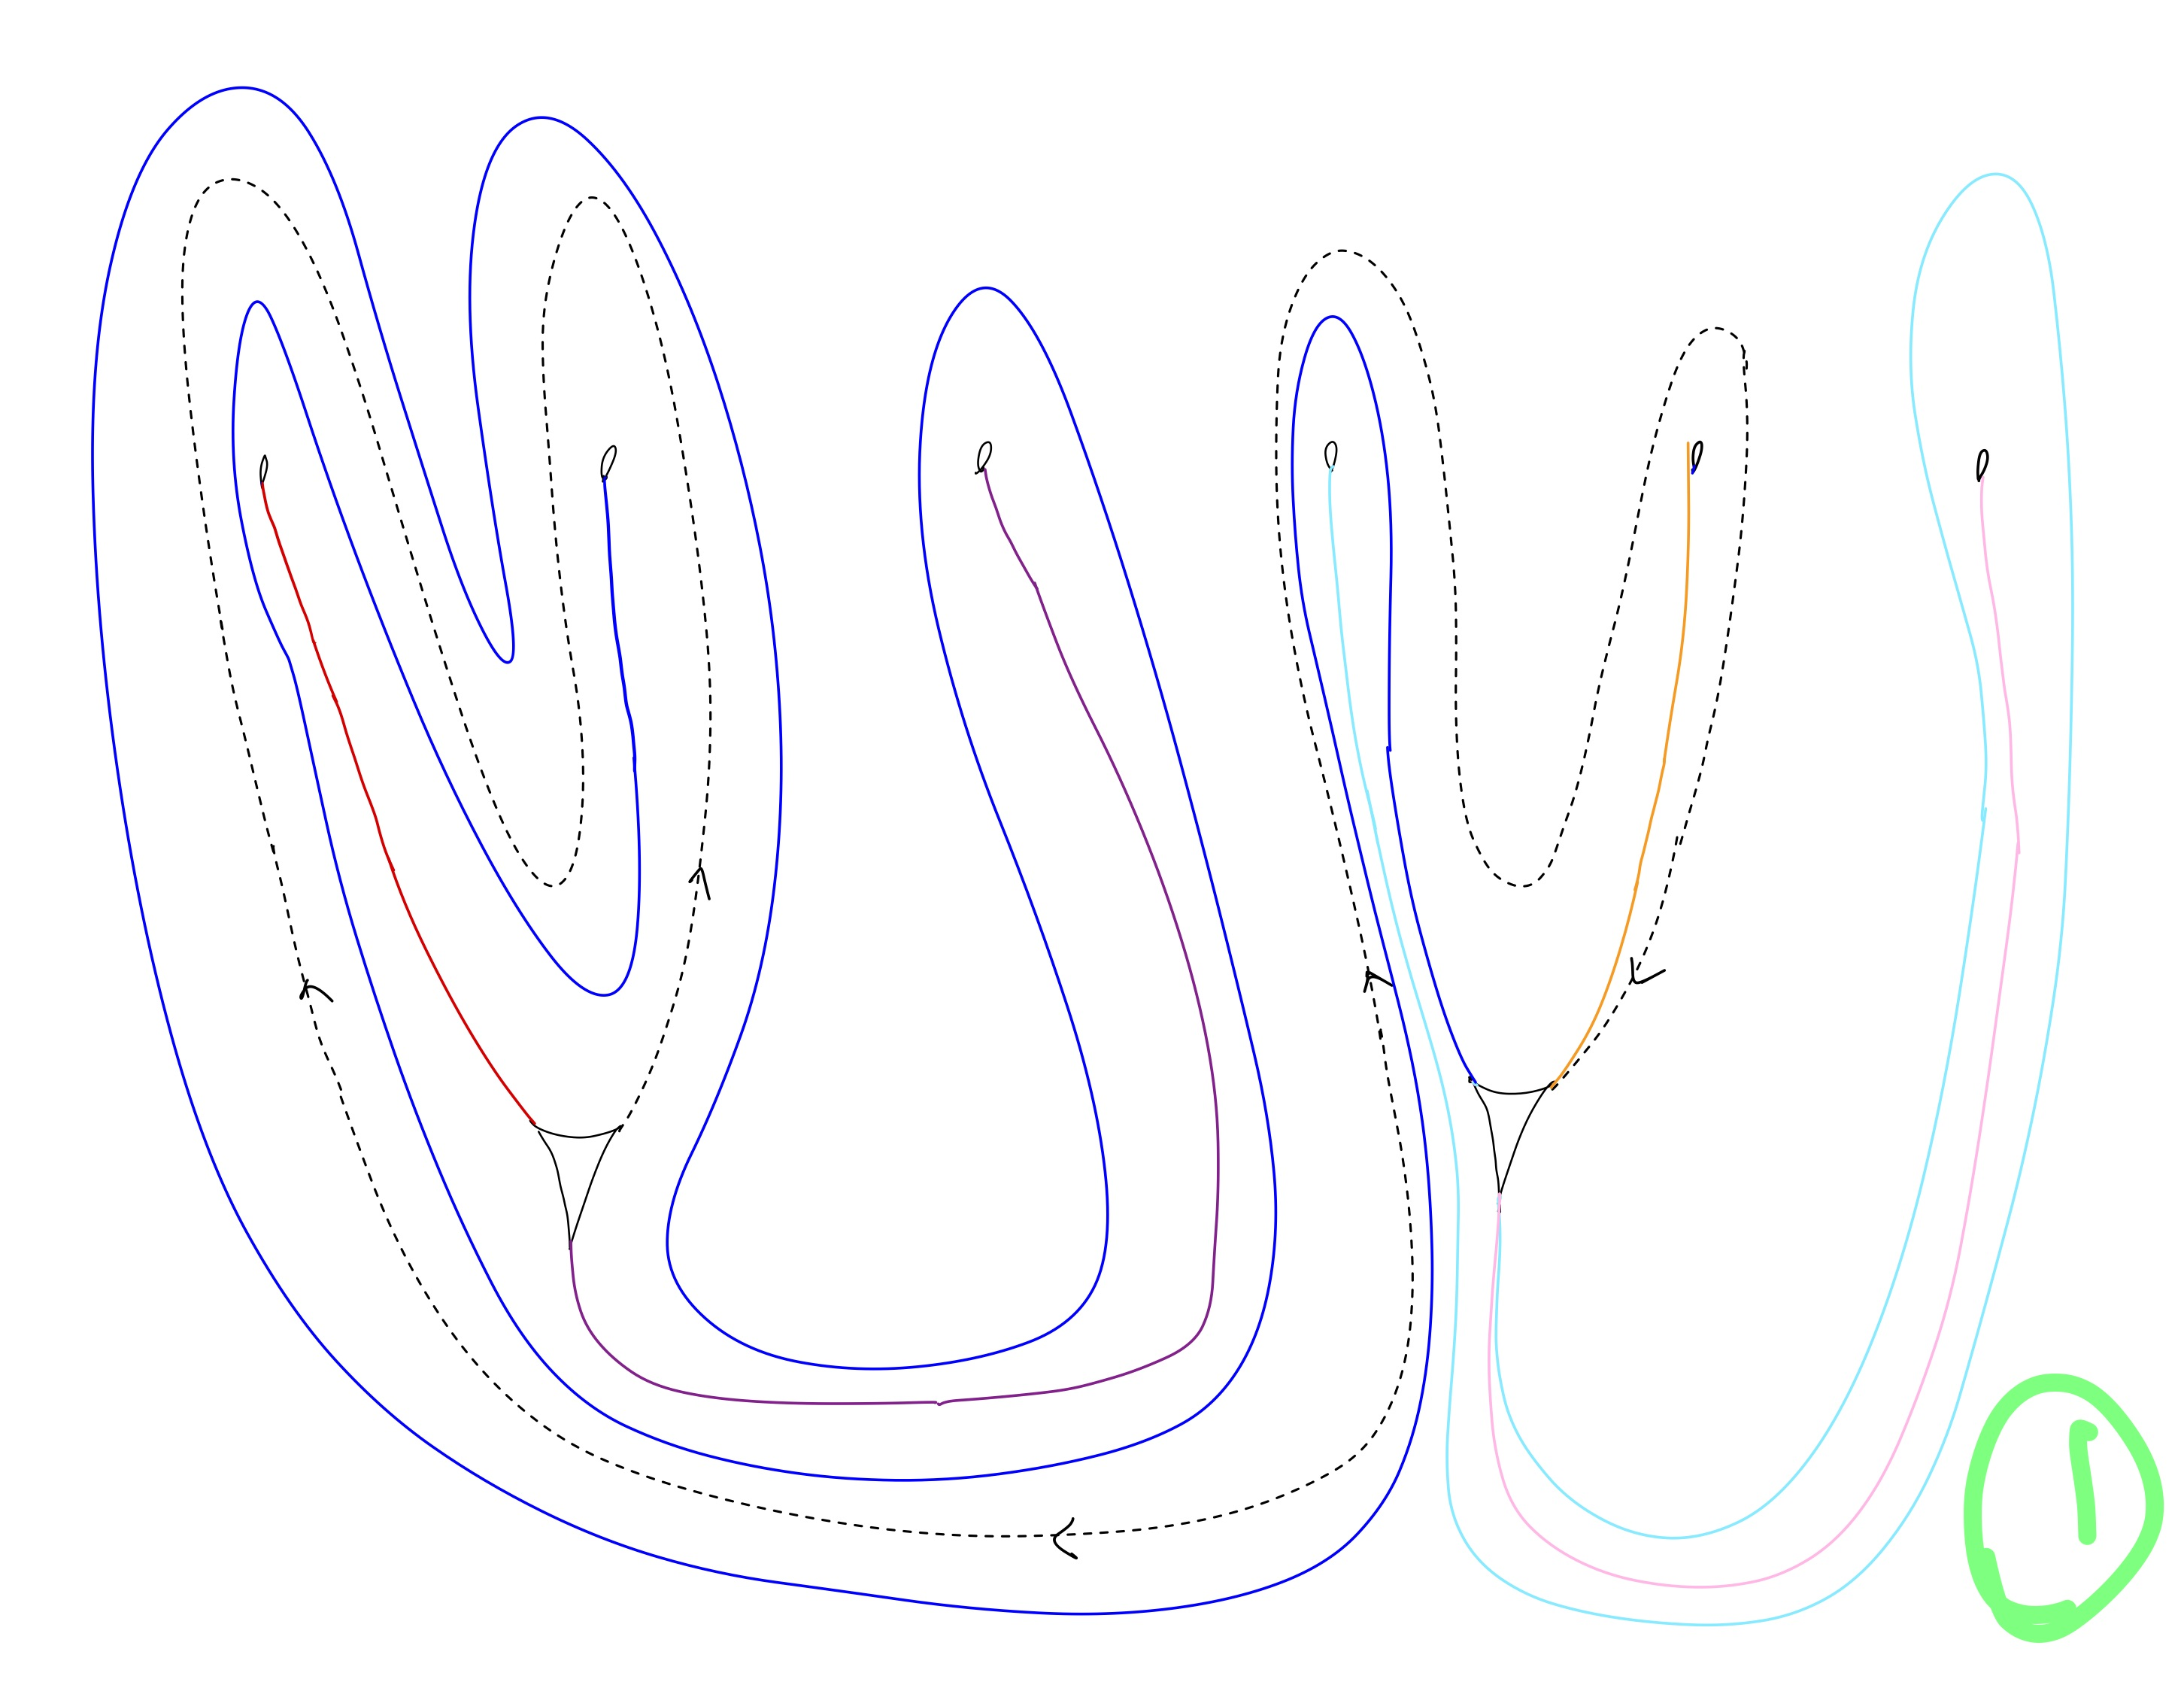
\includegraphics[width=\linewidth, height=0.45\textheight, keepaspectratio]{figures_braid/figures_track_17/Track 17 Braid 1 Cudden-1.jpg}
    \caption{Train Track Map Candidate Family 1 (Cudden) of Track 17.}
    \label{fig:track17_braid_b17_1_map}
\end{figure*}

The inverse of the following braid carries this family of train track maps:
\[
b_1^{17} = \sigma_{1} \sigma_{1} \sigma_{2} \sigma_{2} \sigma_{1} \sigma_{2} \sigma_{4} \sigma_{5} \sigma_{5} \sigma_{4} \sigma_{5} \sigma_{1} \sigma_{2} \sigma_{3} \sigma_{4} \sigma_{5} \sigma_{5}
\]

This is shown in Figure \ref{fig:track17_braid_b17_1}.

\begin{figure*}[p]
    \centering
    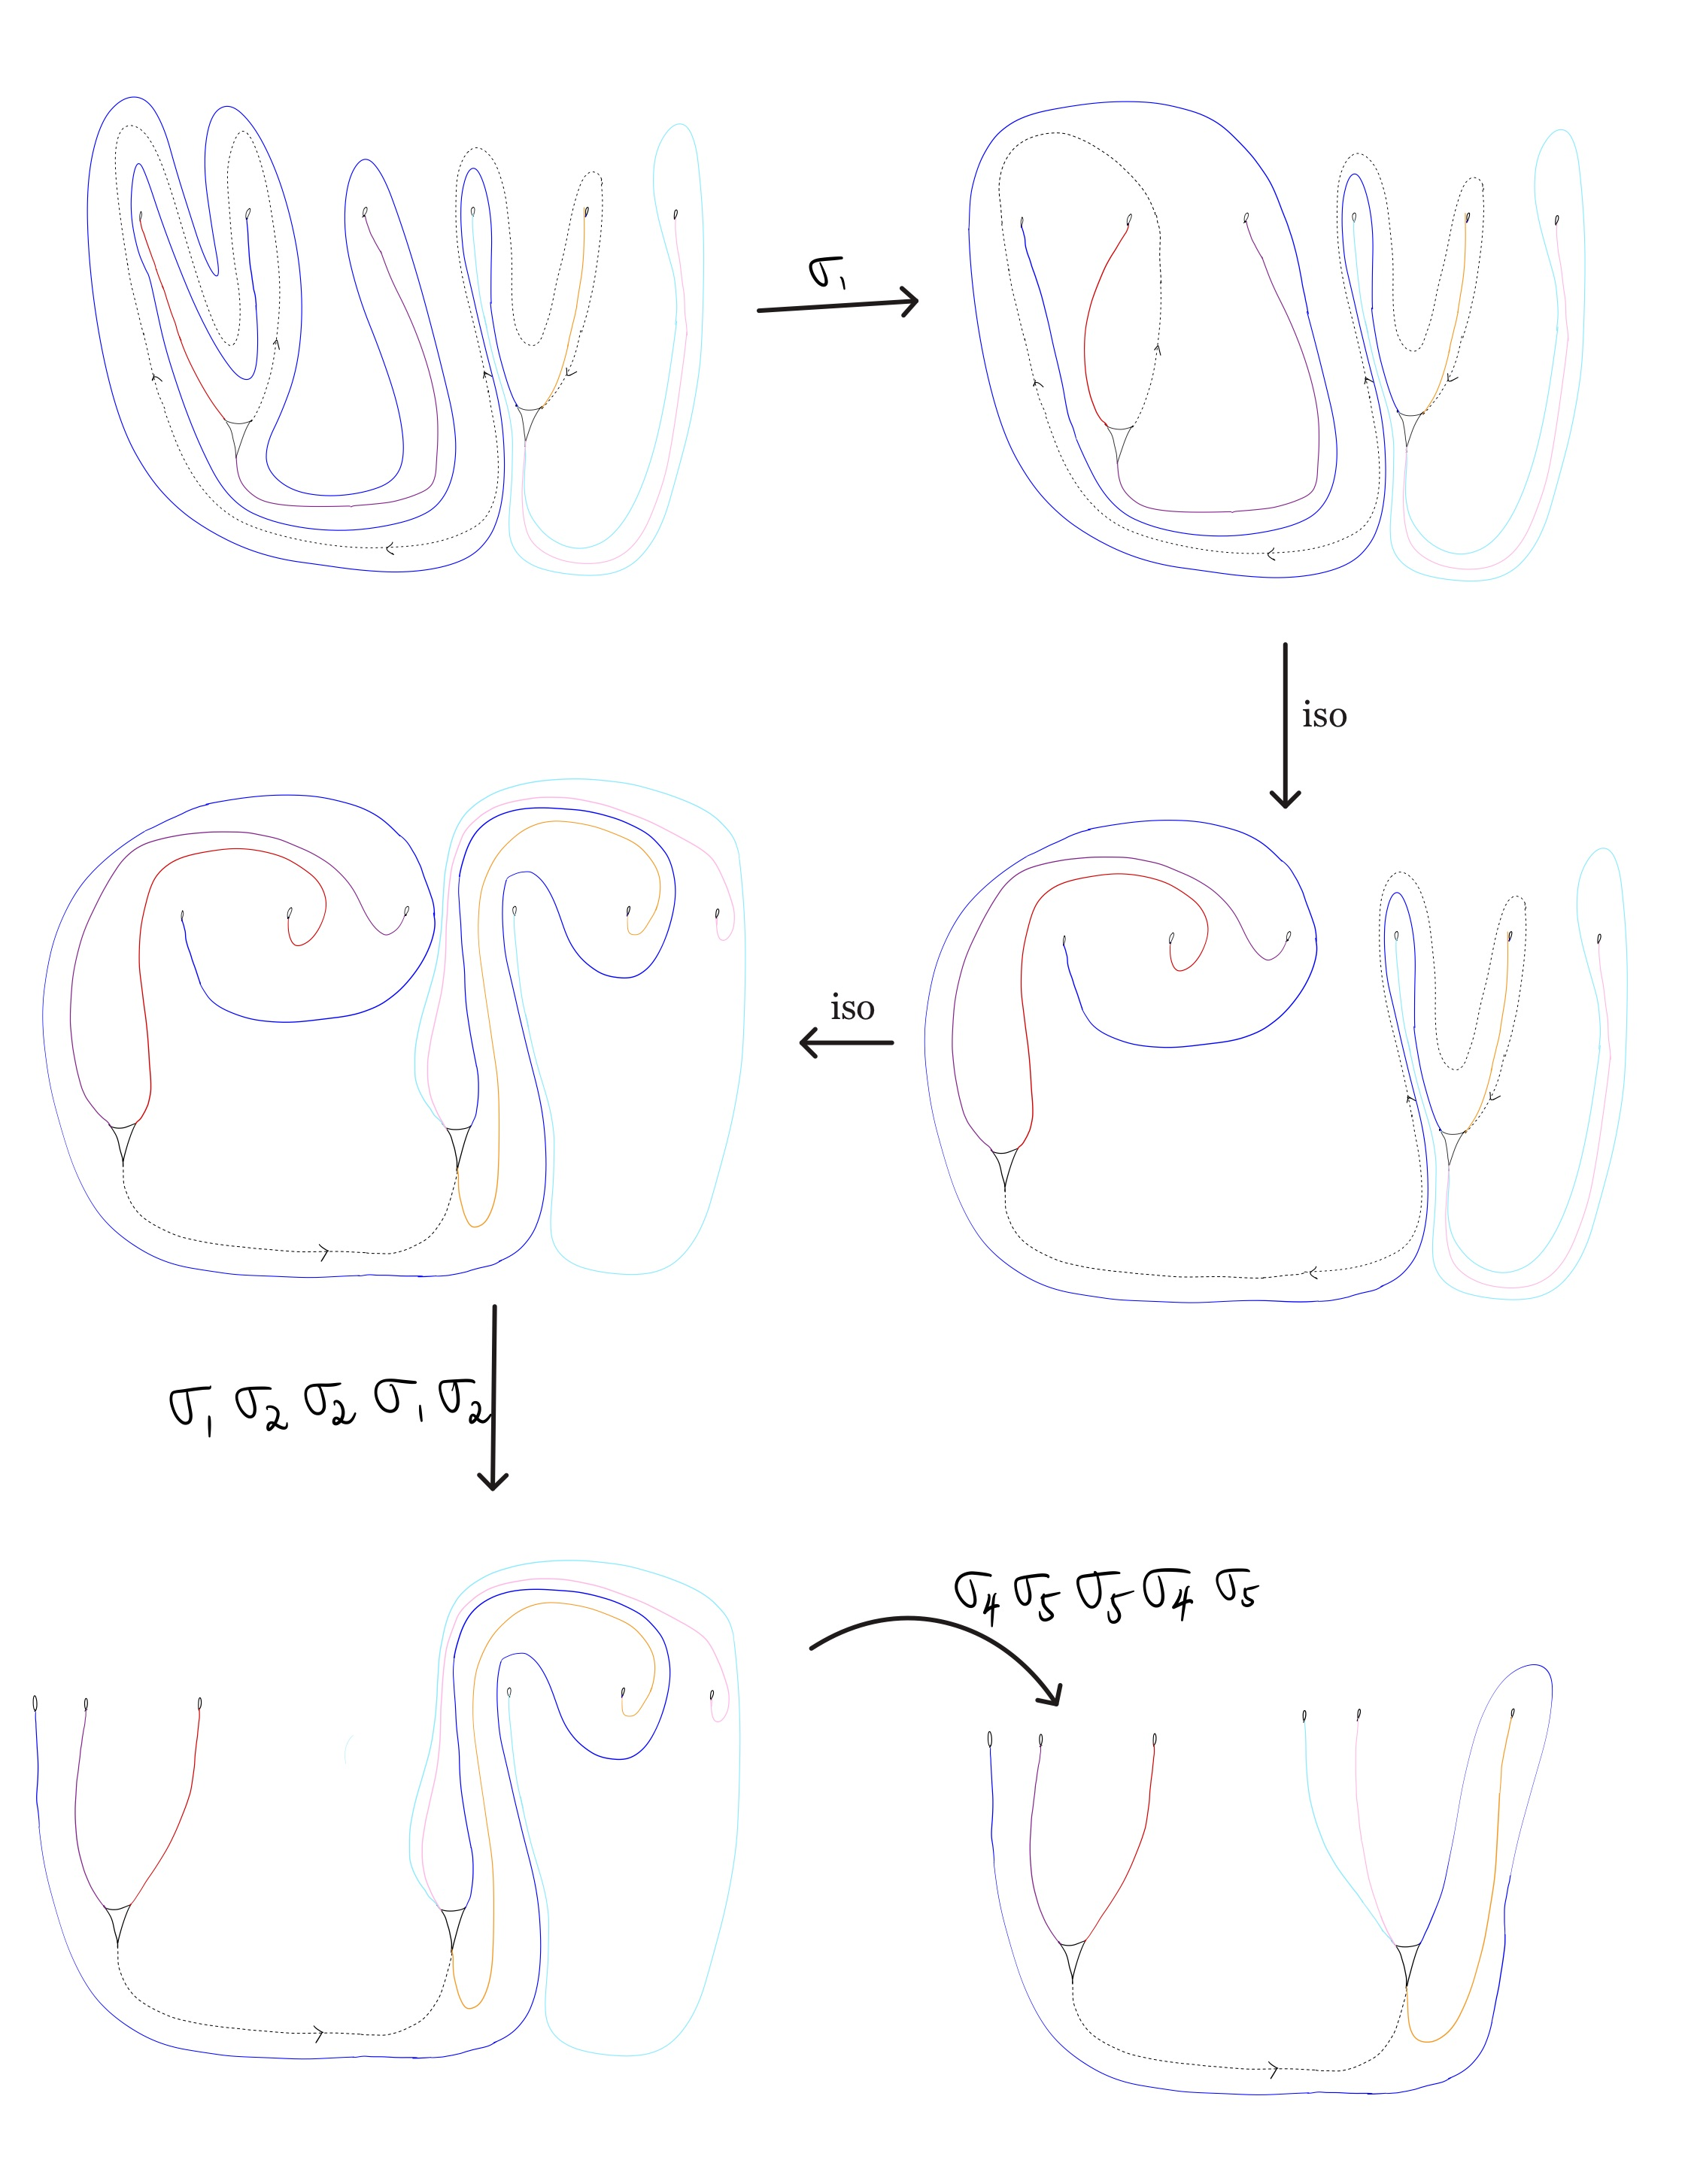
\includegraphics[width=\linewidth, height=0.45\textheight, keepaspectratio]{figures_braid/figures_track_17/Track 17 Braid 1 Cudden-2.jpg}%
    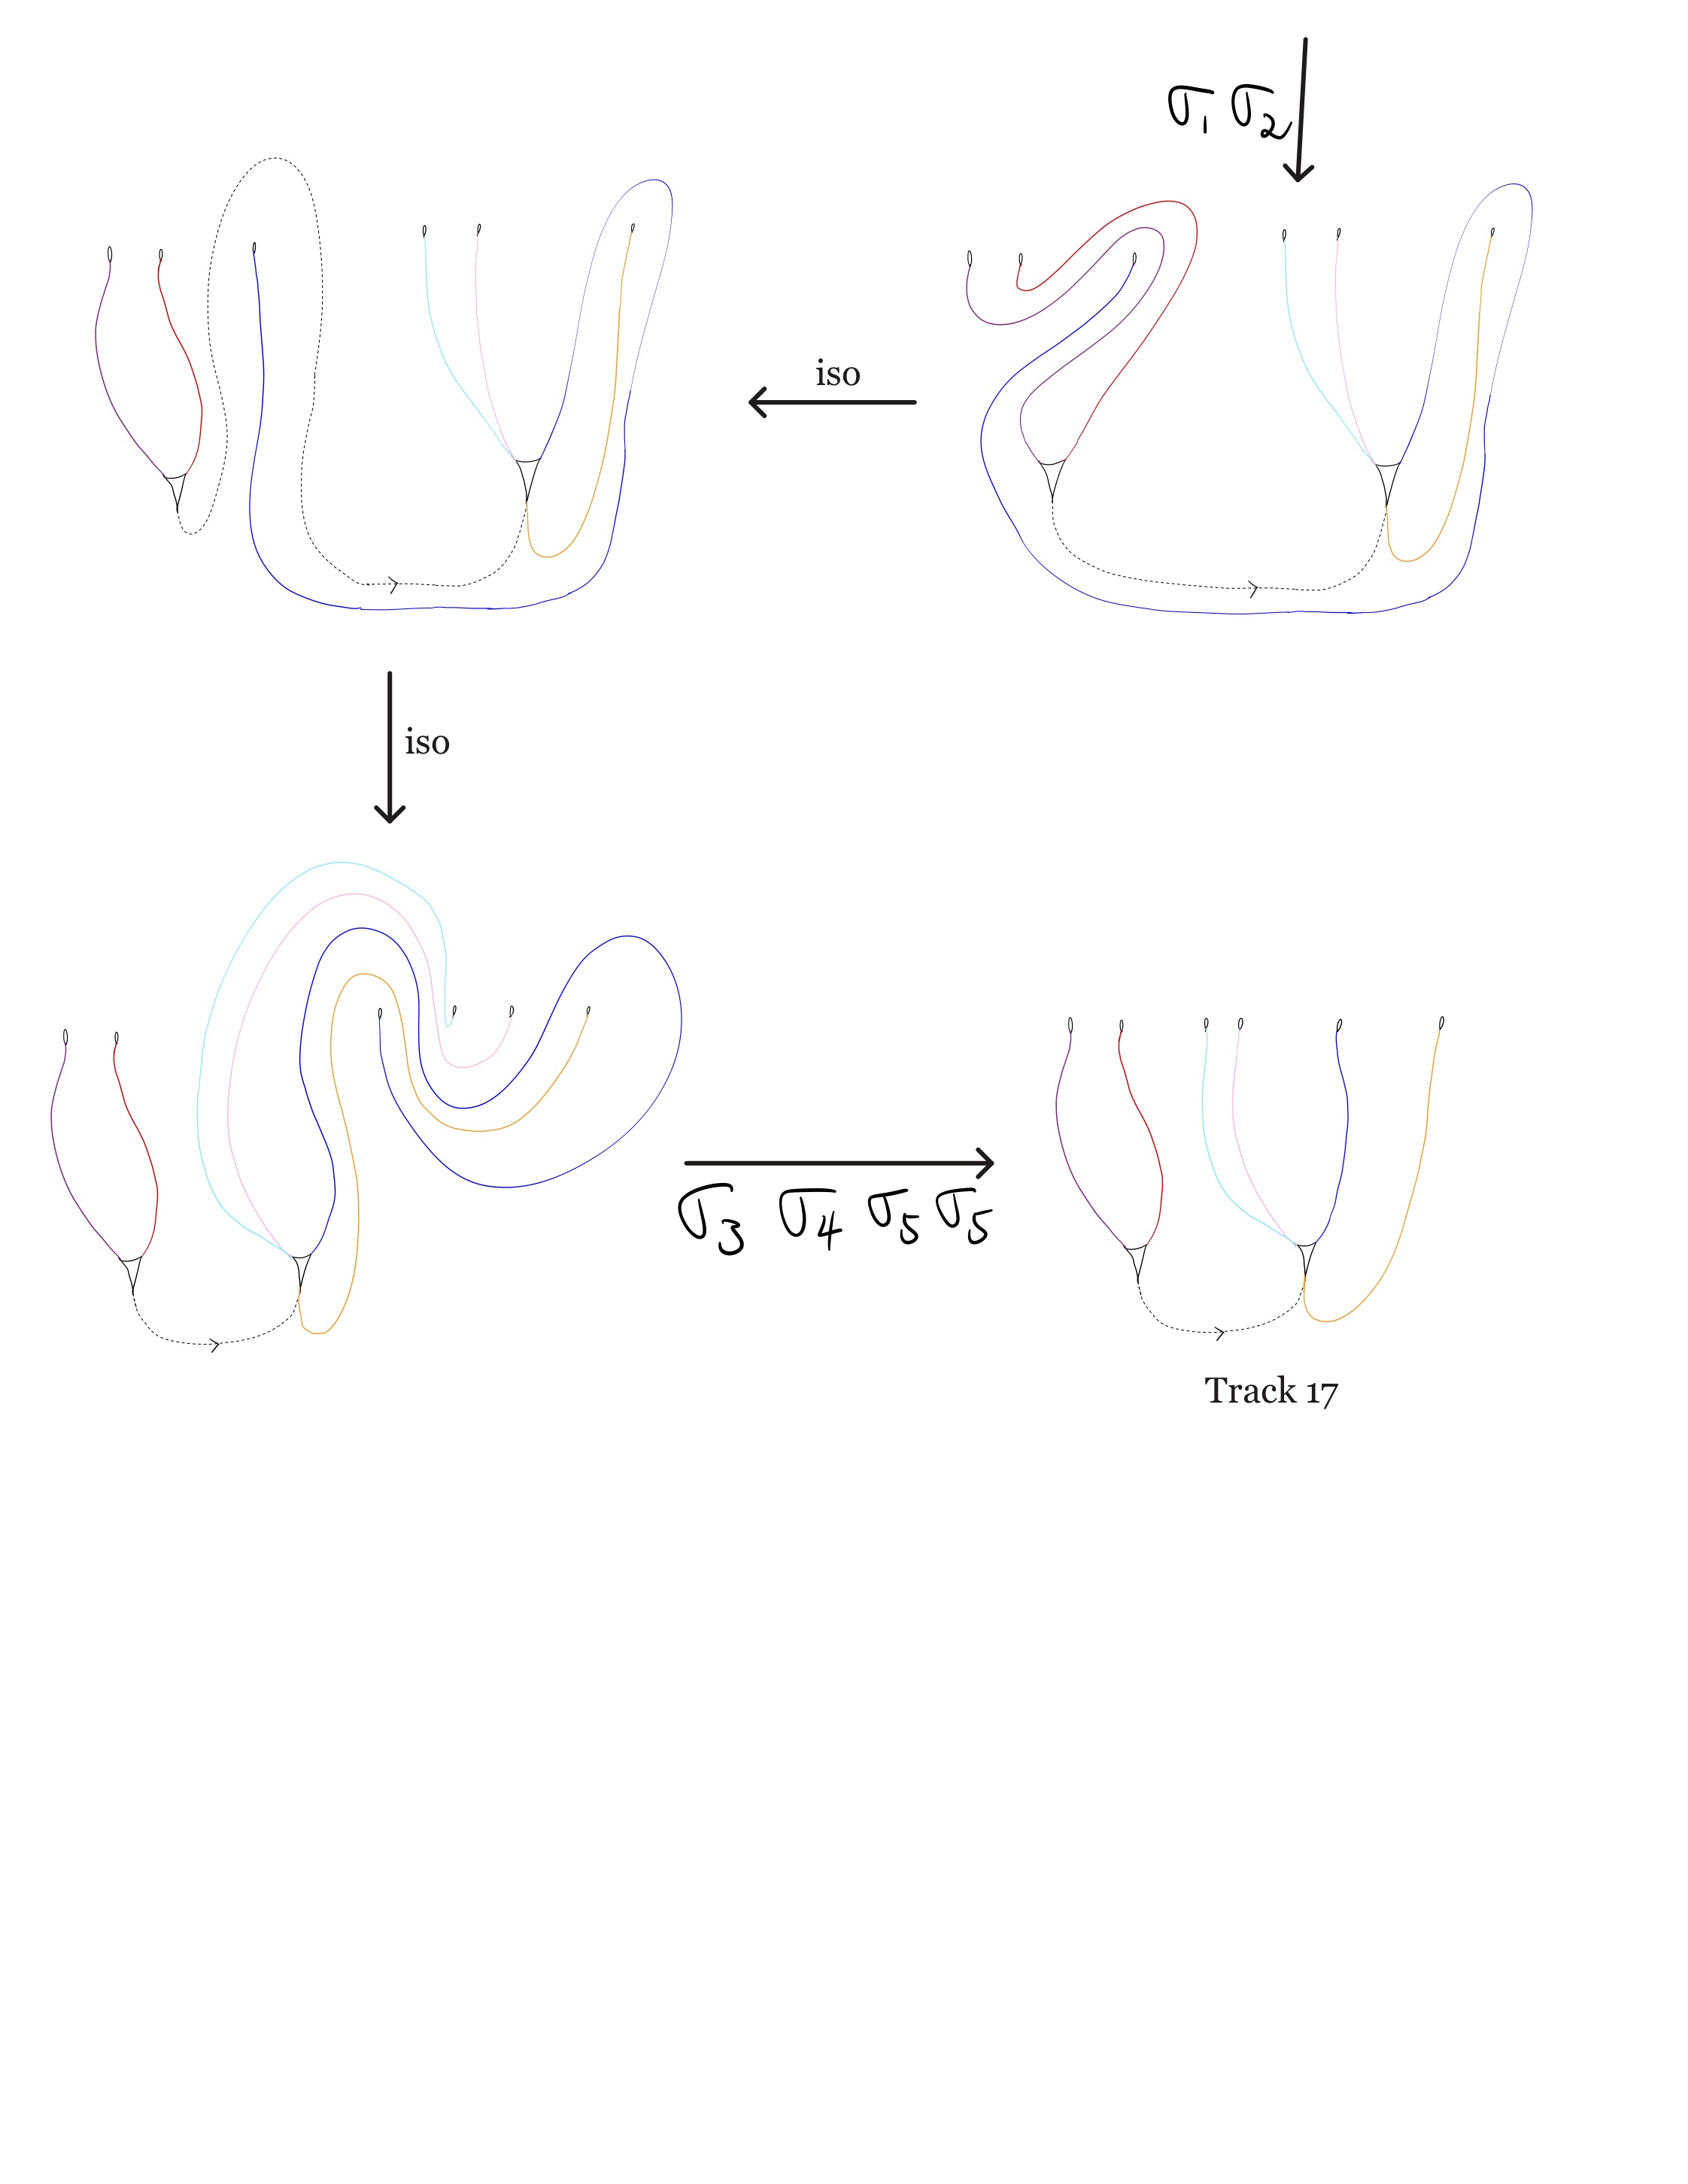
\includegraphics[width=\linewidth, height=0.45\textheight, keepaspectratio]{figures_braid/figures_track_17/Track 17 Braid 1 Cudden-3.jpg}
    \caption{This sequence shows the inverse of the braid $b_1^{17}$ carries Train Track Candidate Family 1.}
    \label{fig:track17_braid_b17_1}
\end{figure*}

\clearpage

\section{Candidate Family 2 (Flisky)}\label{sec:track17_flisky}
Train Track Map Candidate Family 2 of Track 17 is shown in Figure \ref{fig:track17_braid_b17_2_map}. See \ref{Flisky} for details.

\begin{figure*}[ht]
    \centering
    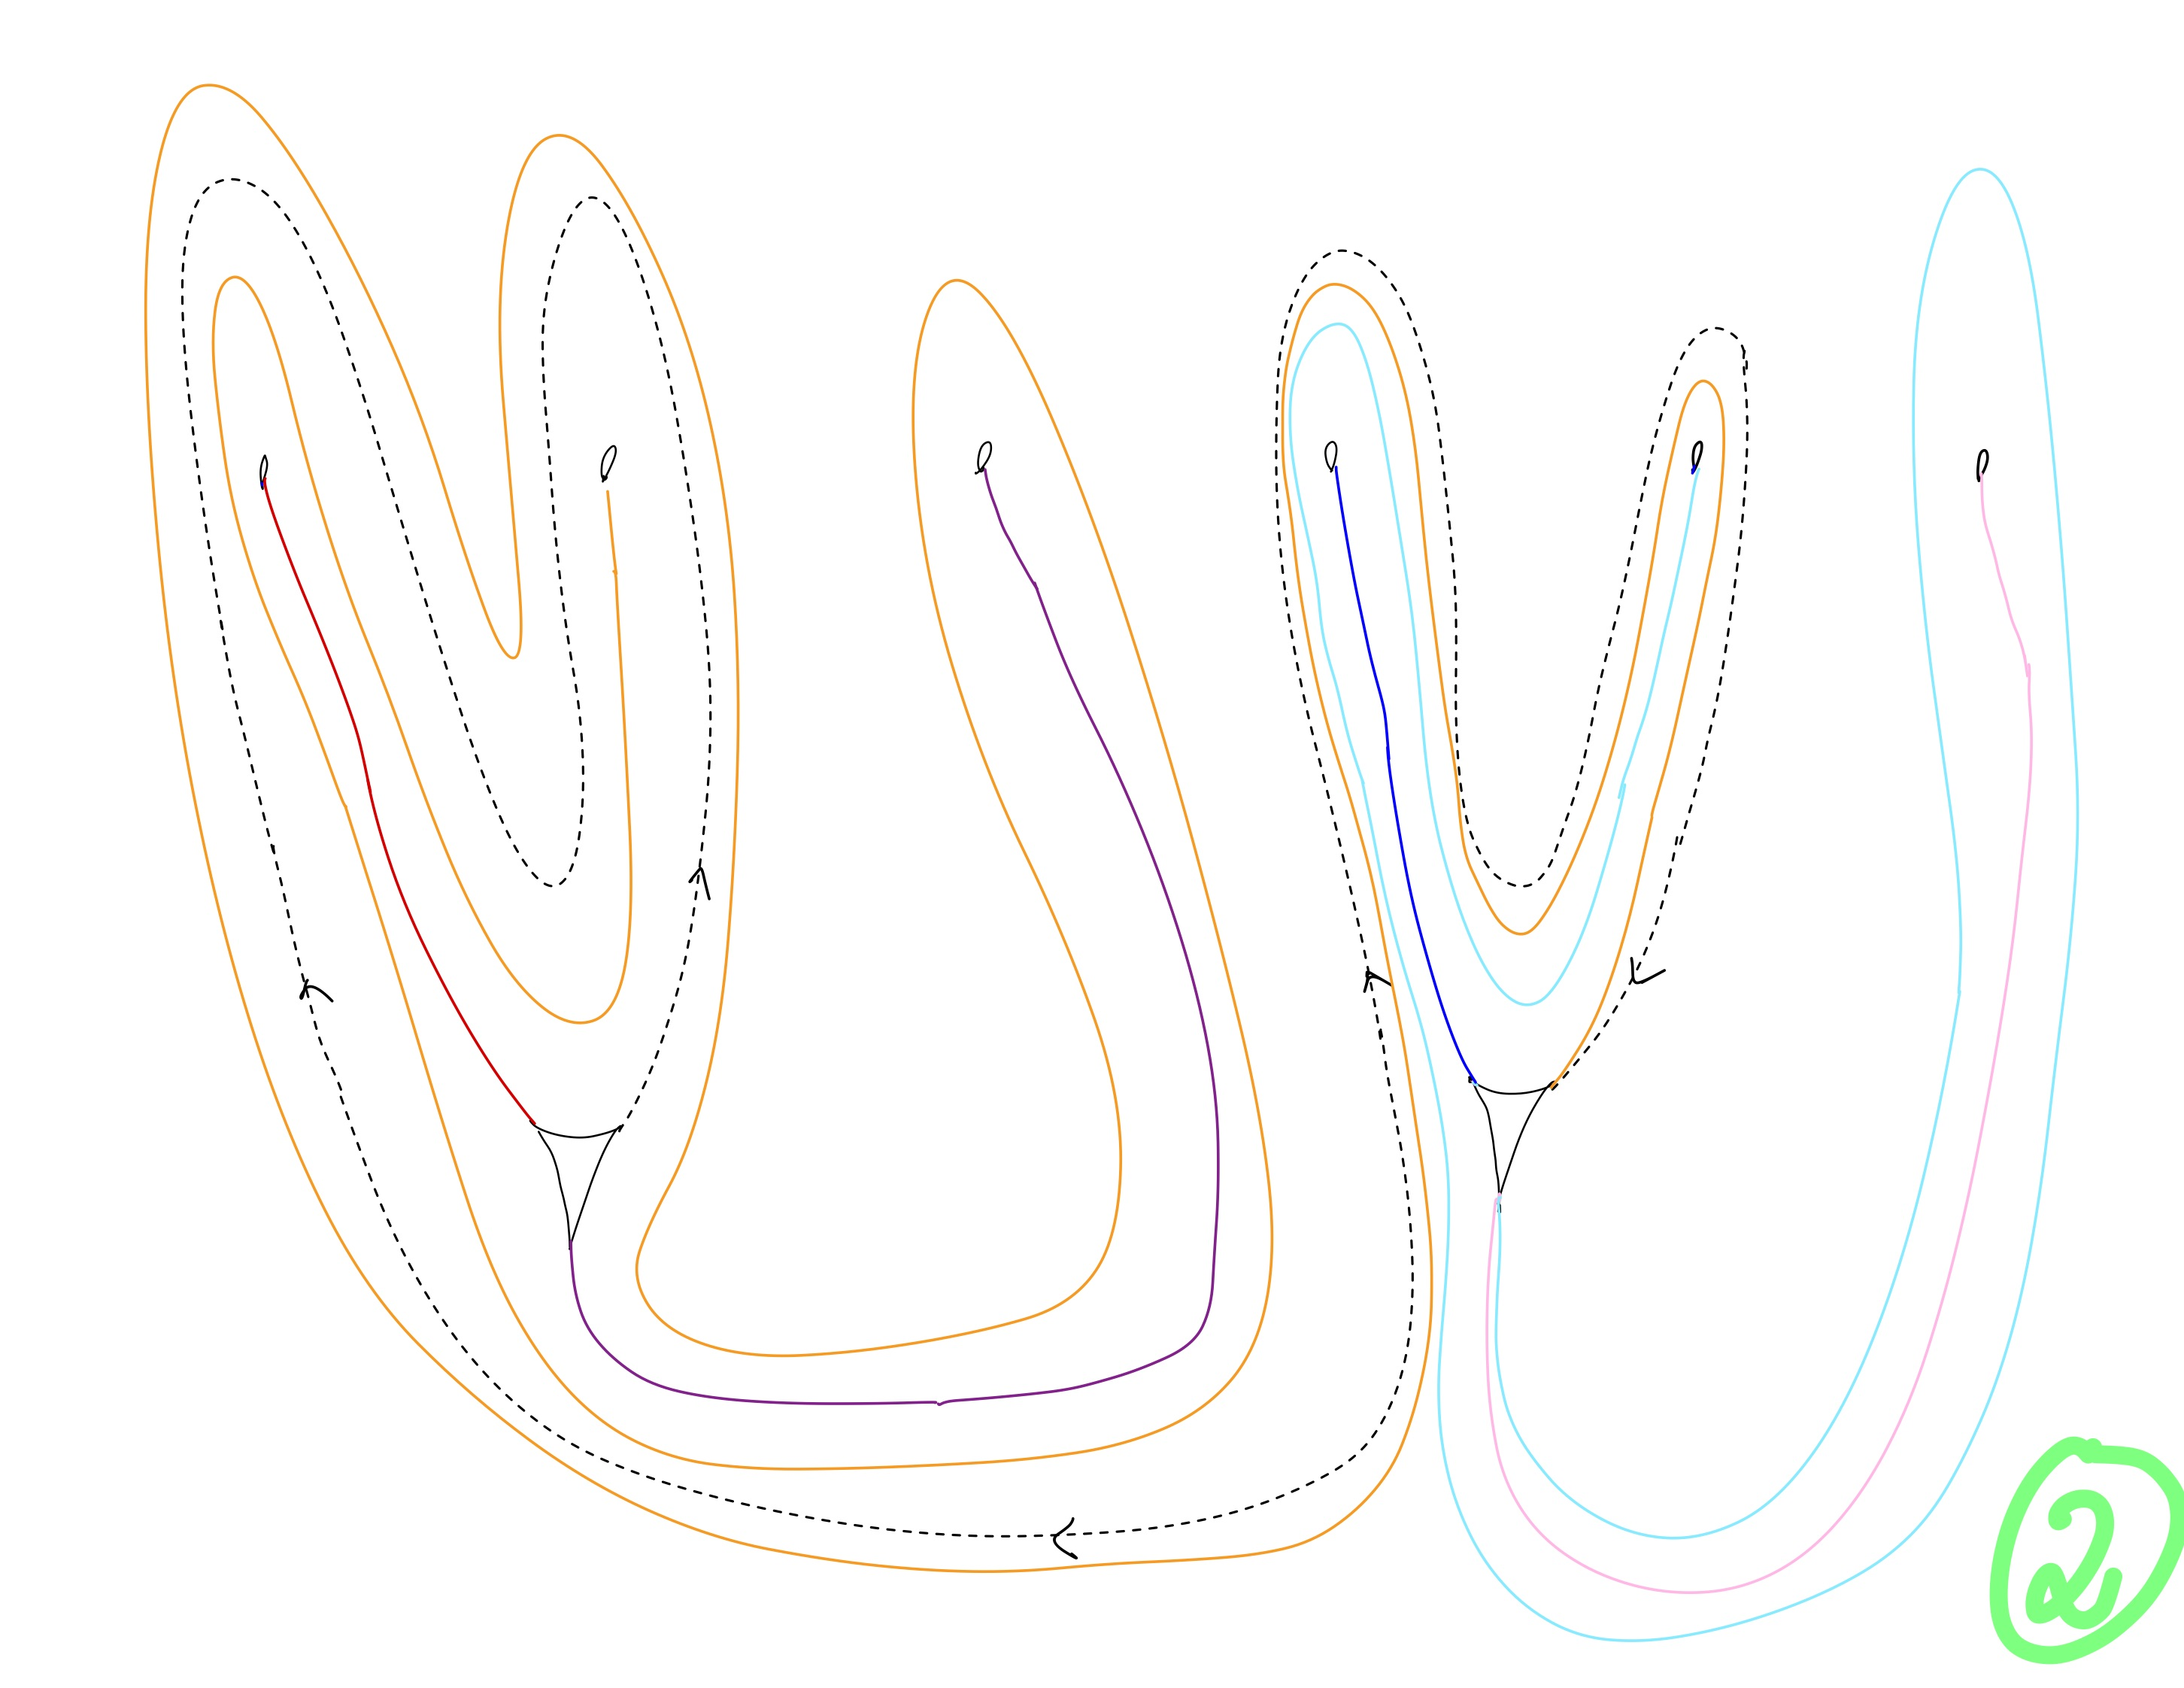
\includegraphics[width=\linewidth, height=0.45\textheight, keepaspectratio]{figures_braid/figures_track_17/Track 17 Braid 2 Flisky-1.jpg}
    \caption{Train Track Map Candidate Family 2 (Flisky) of Track 17.}
    \label{fig:track17_braid_b17_2_map}
\end{figure*}

The inverse of the following braid carries this family of train track maps:
\[
b_2^{17} = \sigma_{1} \sigma_{4} \sigma_{1} \sigma_{2} \sigma_{2} \sigma_{1} \sigma_{2} \sigma_{4} \sigma_{5} \sigma_{5} \sigma_{4} \sigma_{5} \sigma_{1} \sigma_{2} \sigma_{3} \sigma_{4} \sigma_{5}
\]

This is shown in Figure \ref{fig:track17_braid_b17_2}.

\begin{figure*}[p]
    \centering
    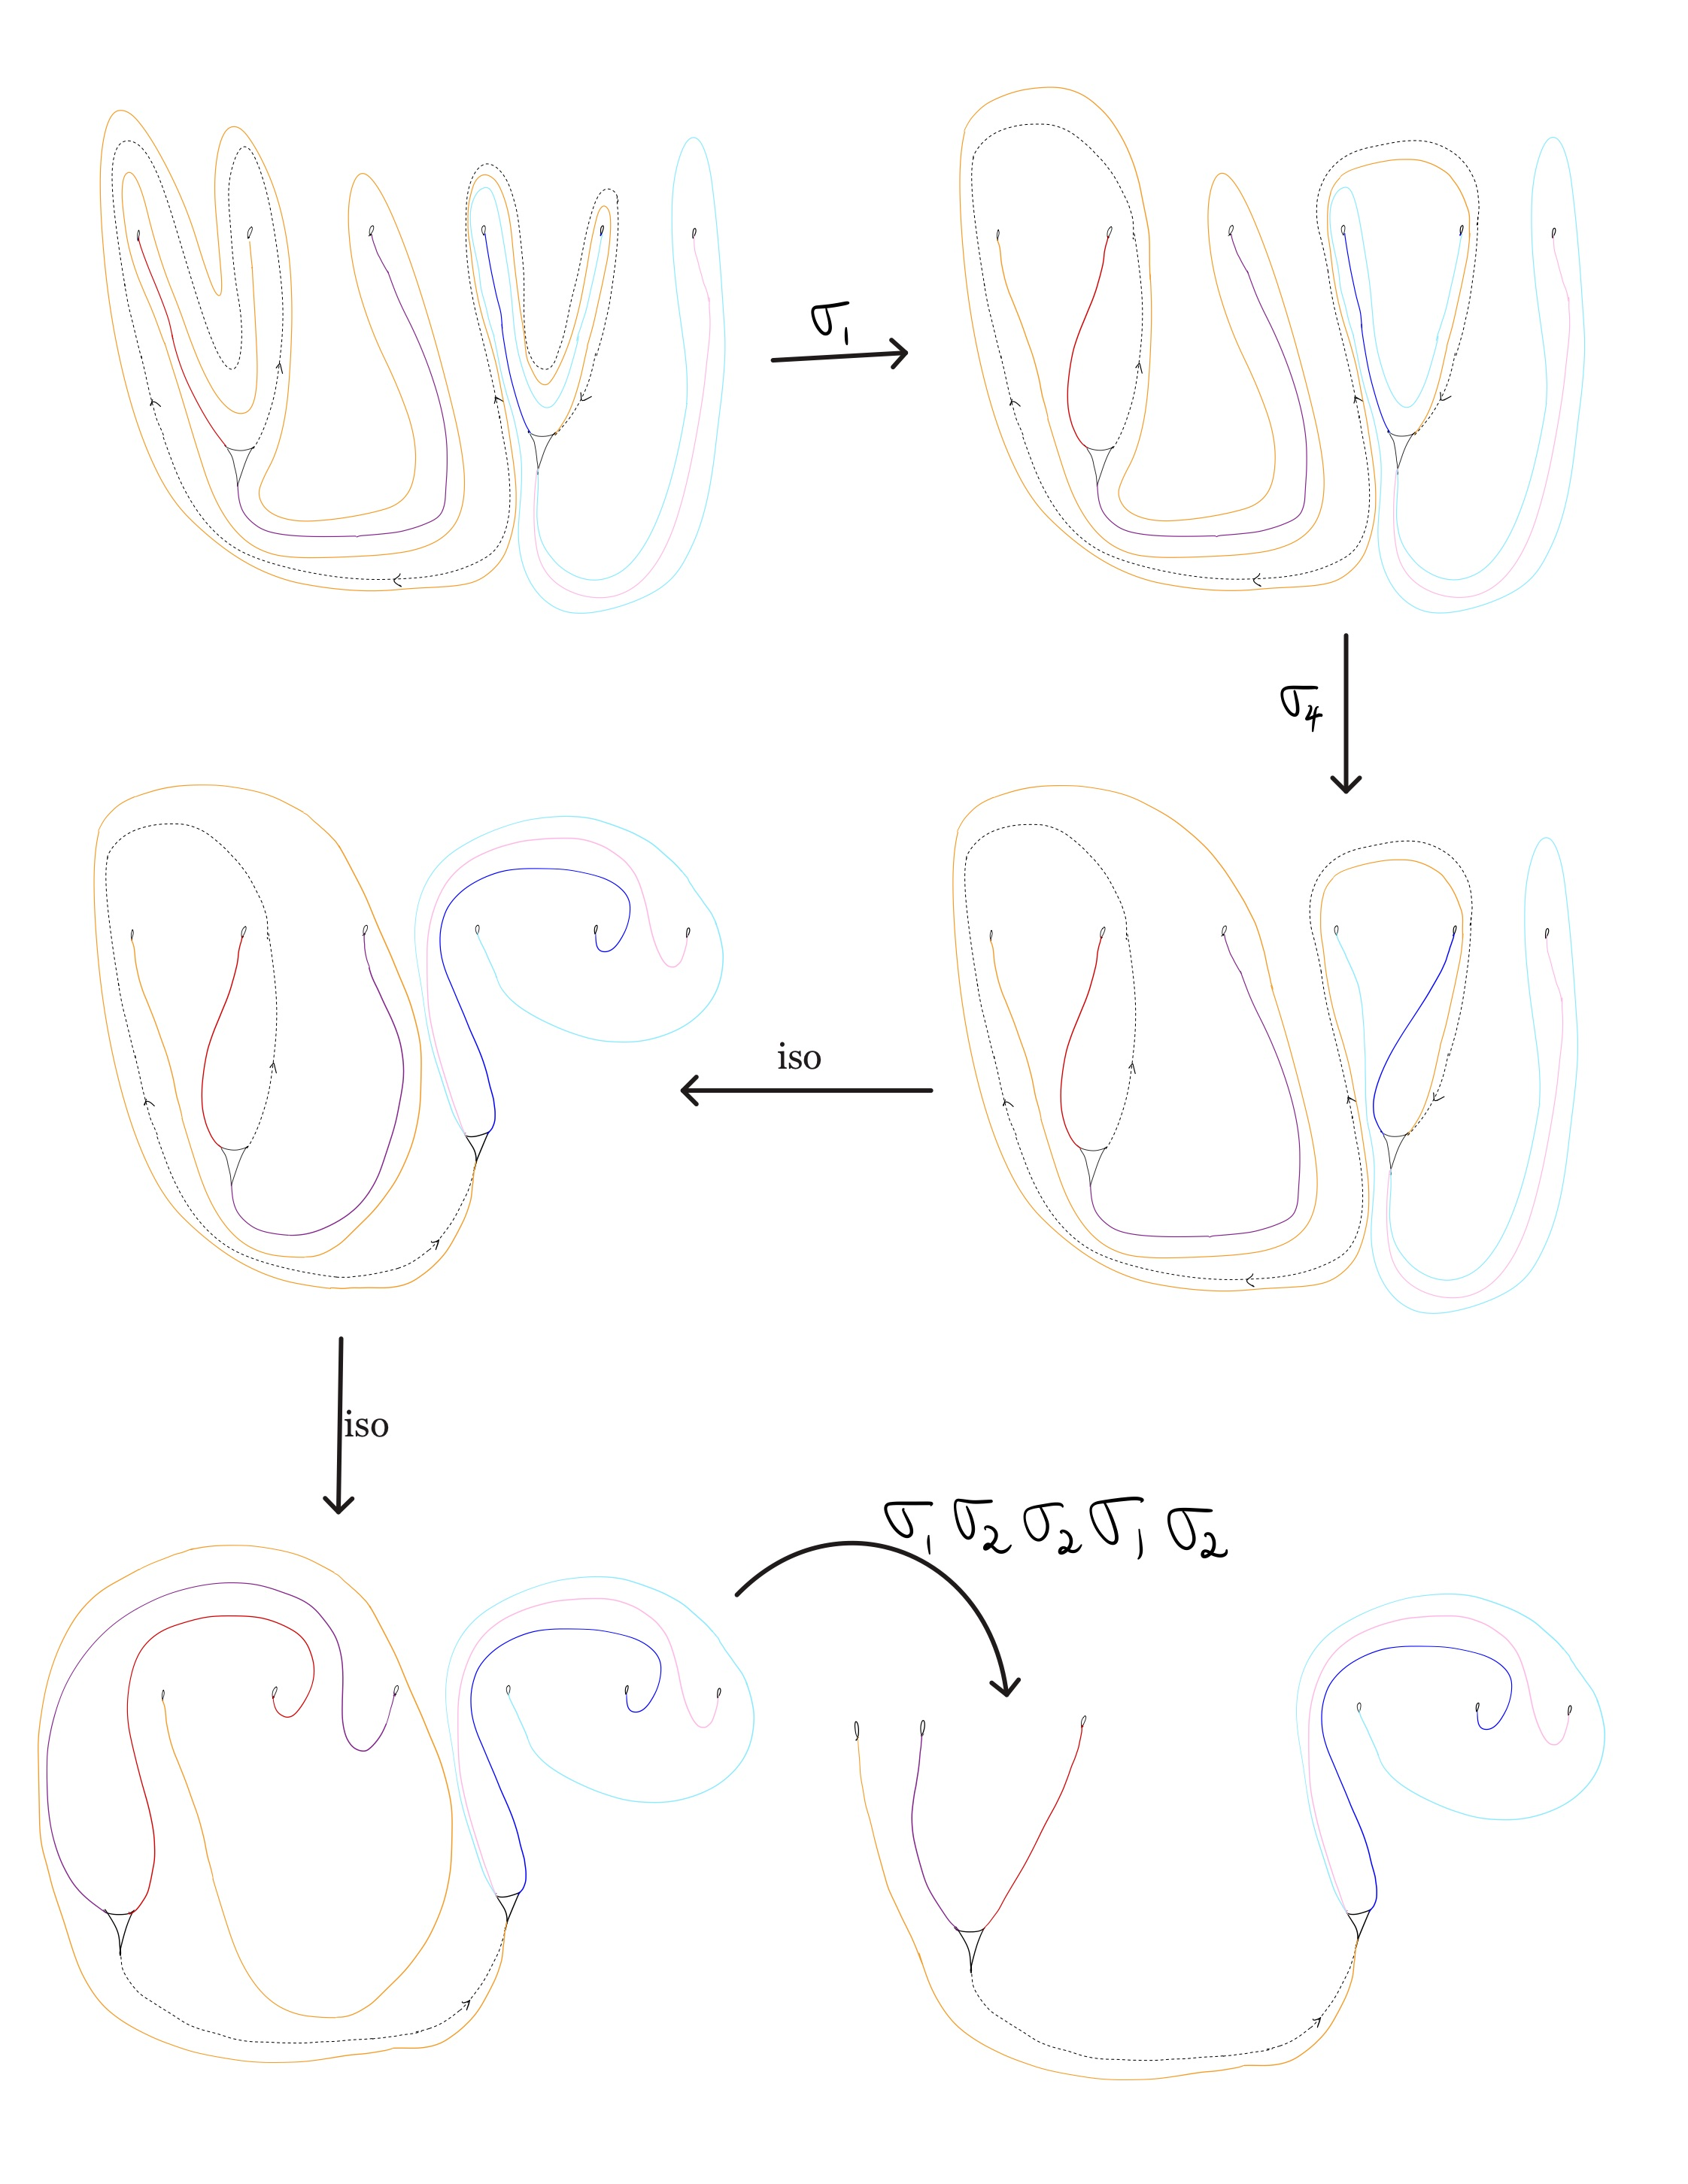
\includegraphics[width=\linewidth, height=0.45\textheight, keepaspectratio]{figures_braid/figures_track_17/Track 17 Braid 2 Flisky-2.jpg}\\
    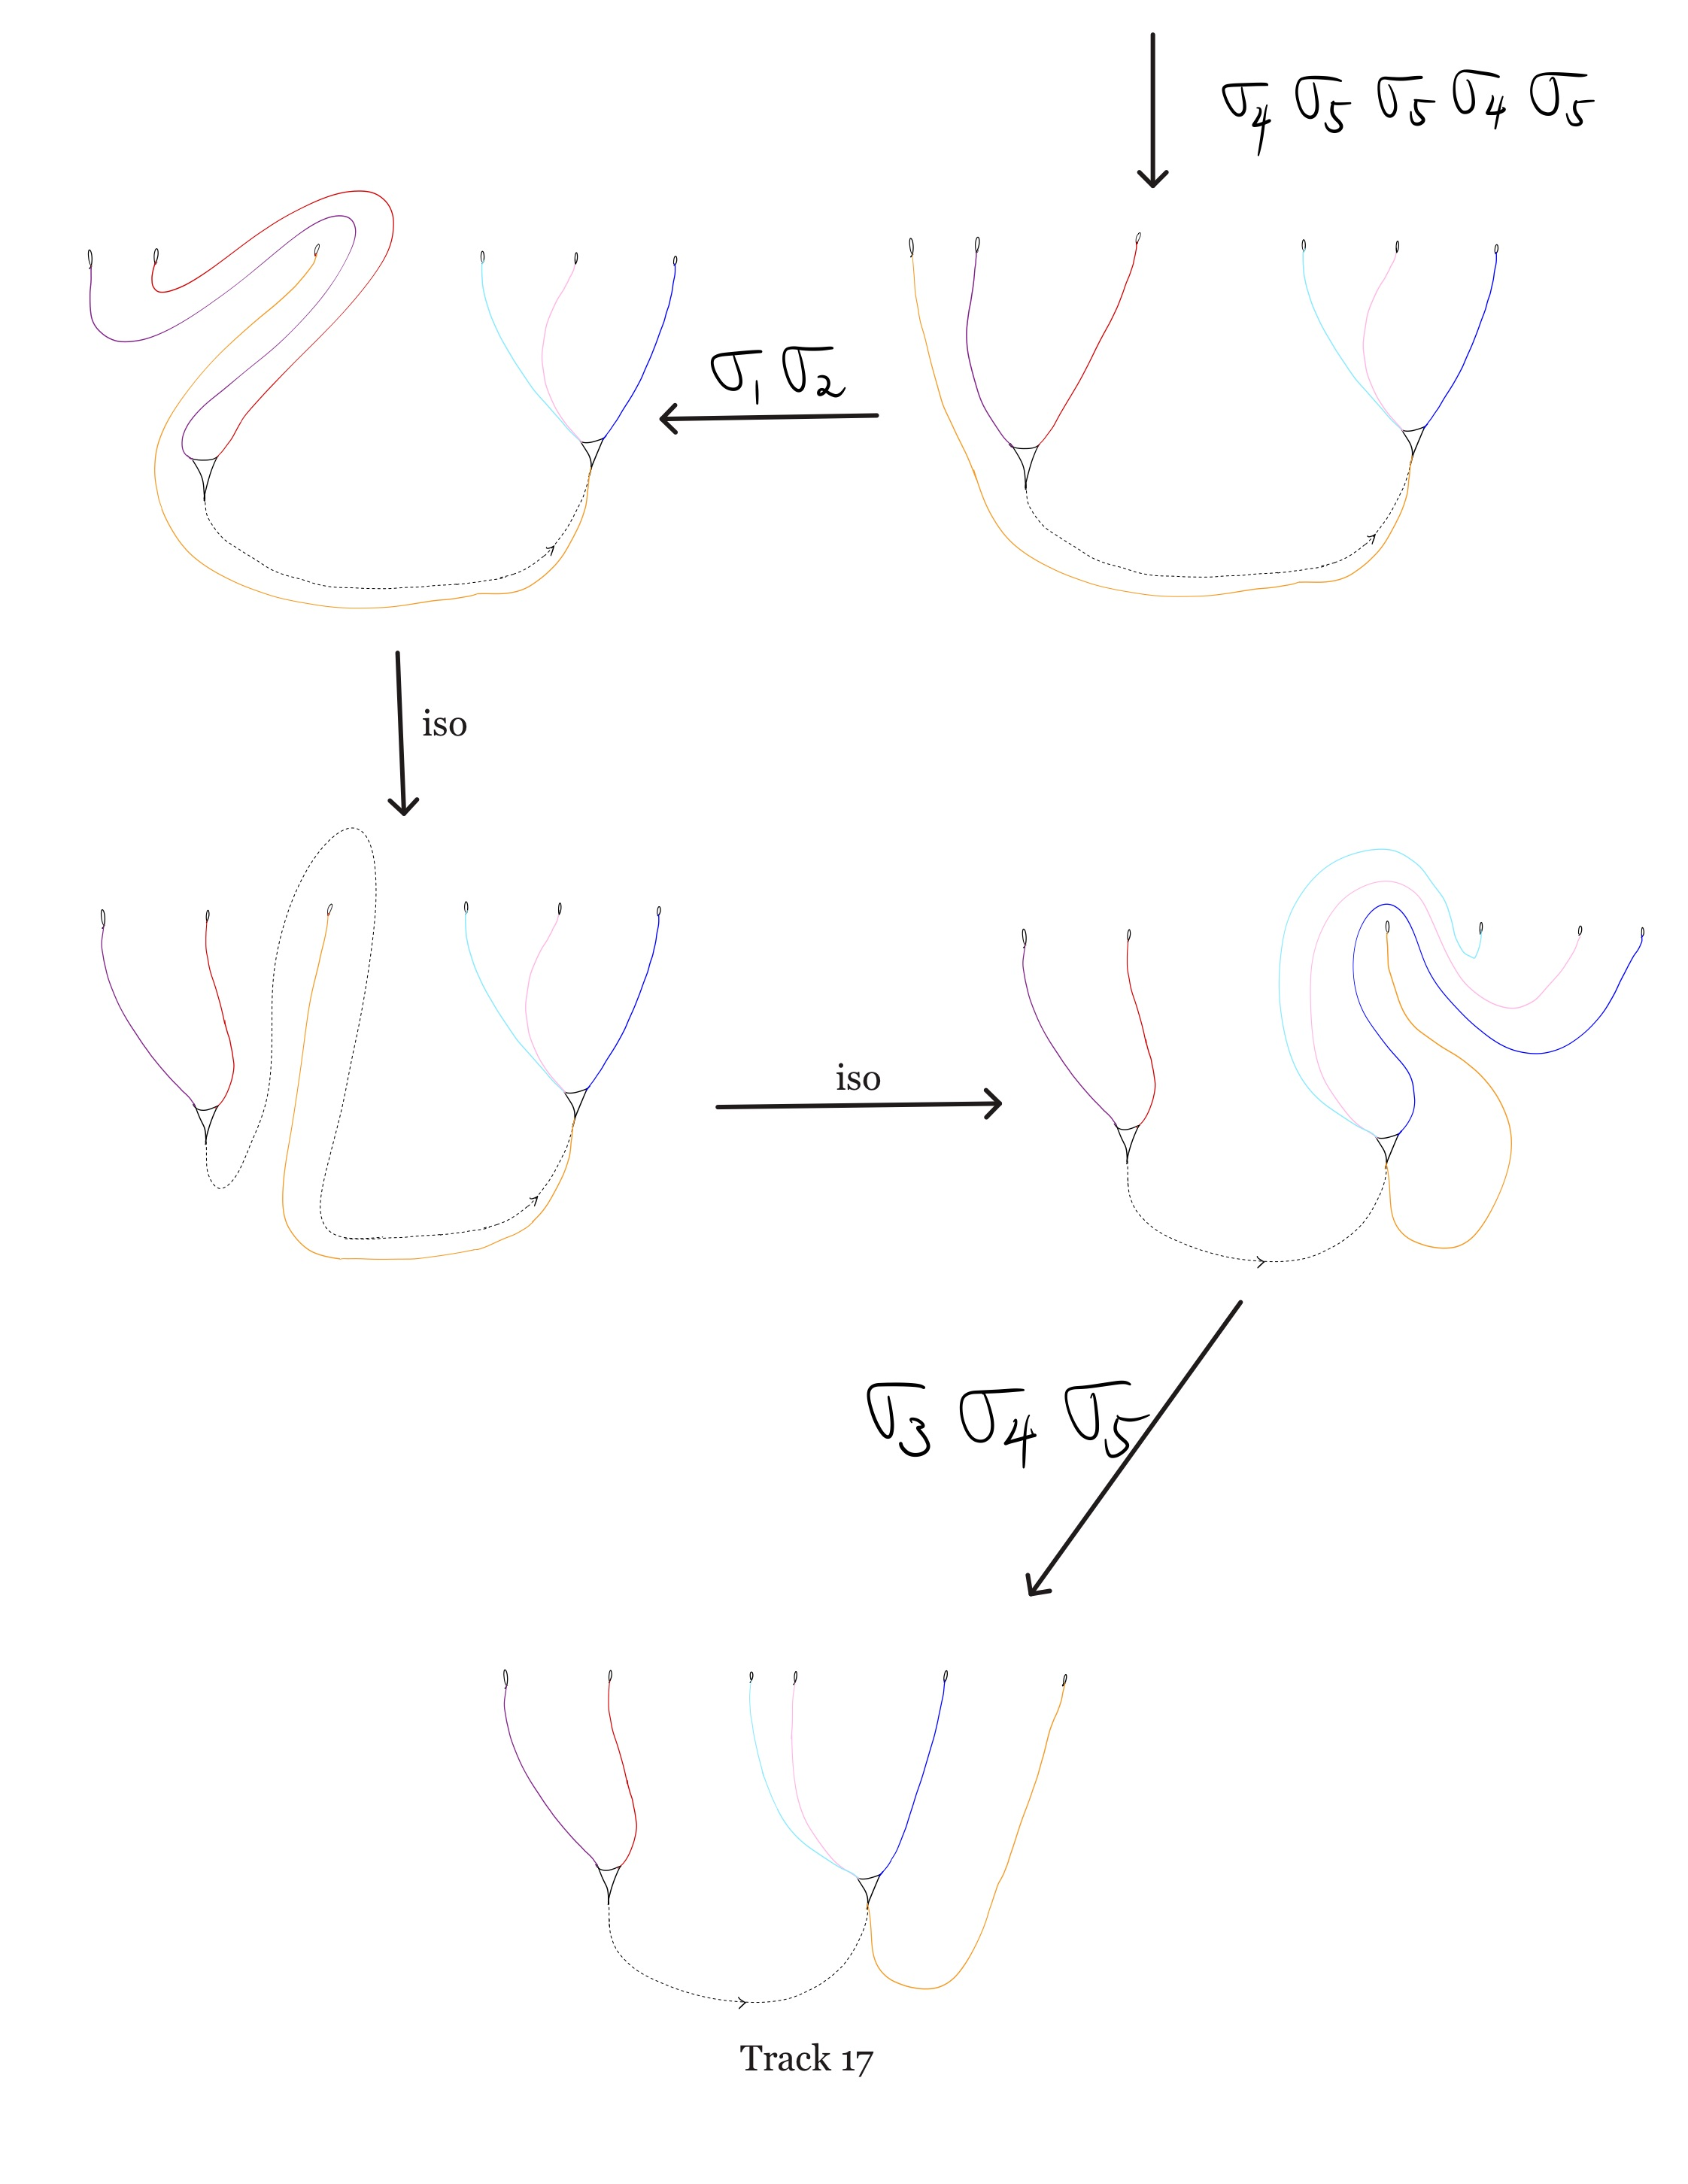
\includegraphics[width=\linewidth, height=0.45\textheight, keepaspectratio]{figures_braid/figures_track_17/Track 17 Braid 2 Flisky-3.jpg}
    \caption{This sequence shows the inverse of the braid $b_2^{17}$ carries Train Track Candidate Family 2.}
    \label{fig:track17_braid_b17_2}
\end{figure*}

\clearpage

\section{Candidate Family 3 (Wanion)}\label{sec:track17_wanion}
Train Track Map Candidate Family 3 of Track 17 is shown in Figure \ref{fig:track17_braid_b17_3_map}. See \ref{Wanion} for details.

\begin{figure*}[ht]
    \centering
    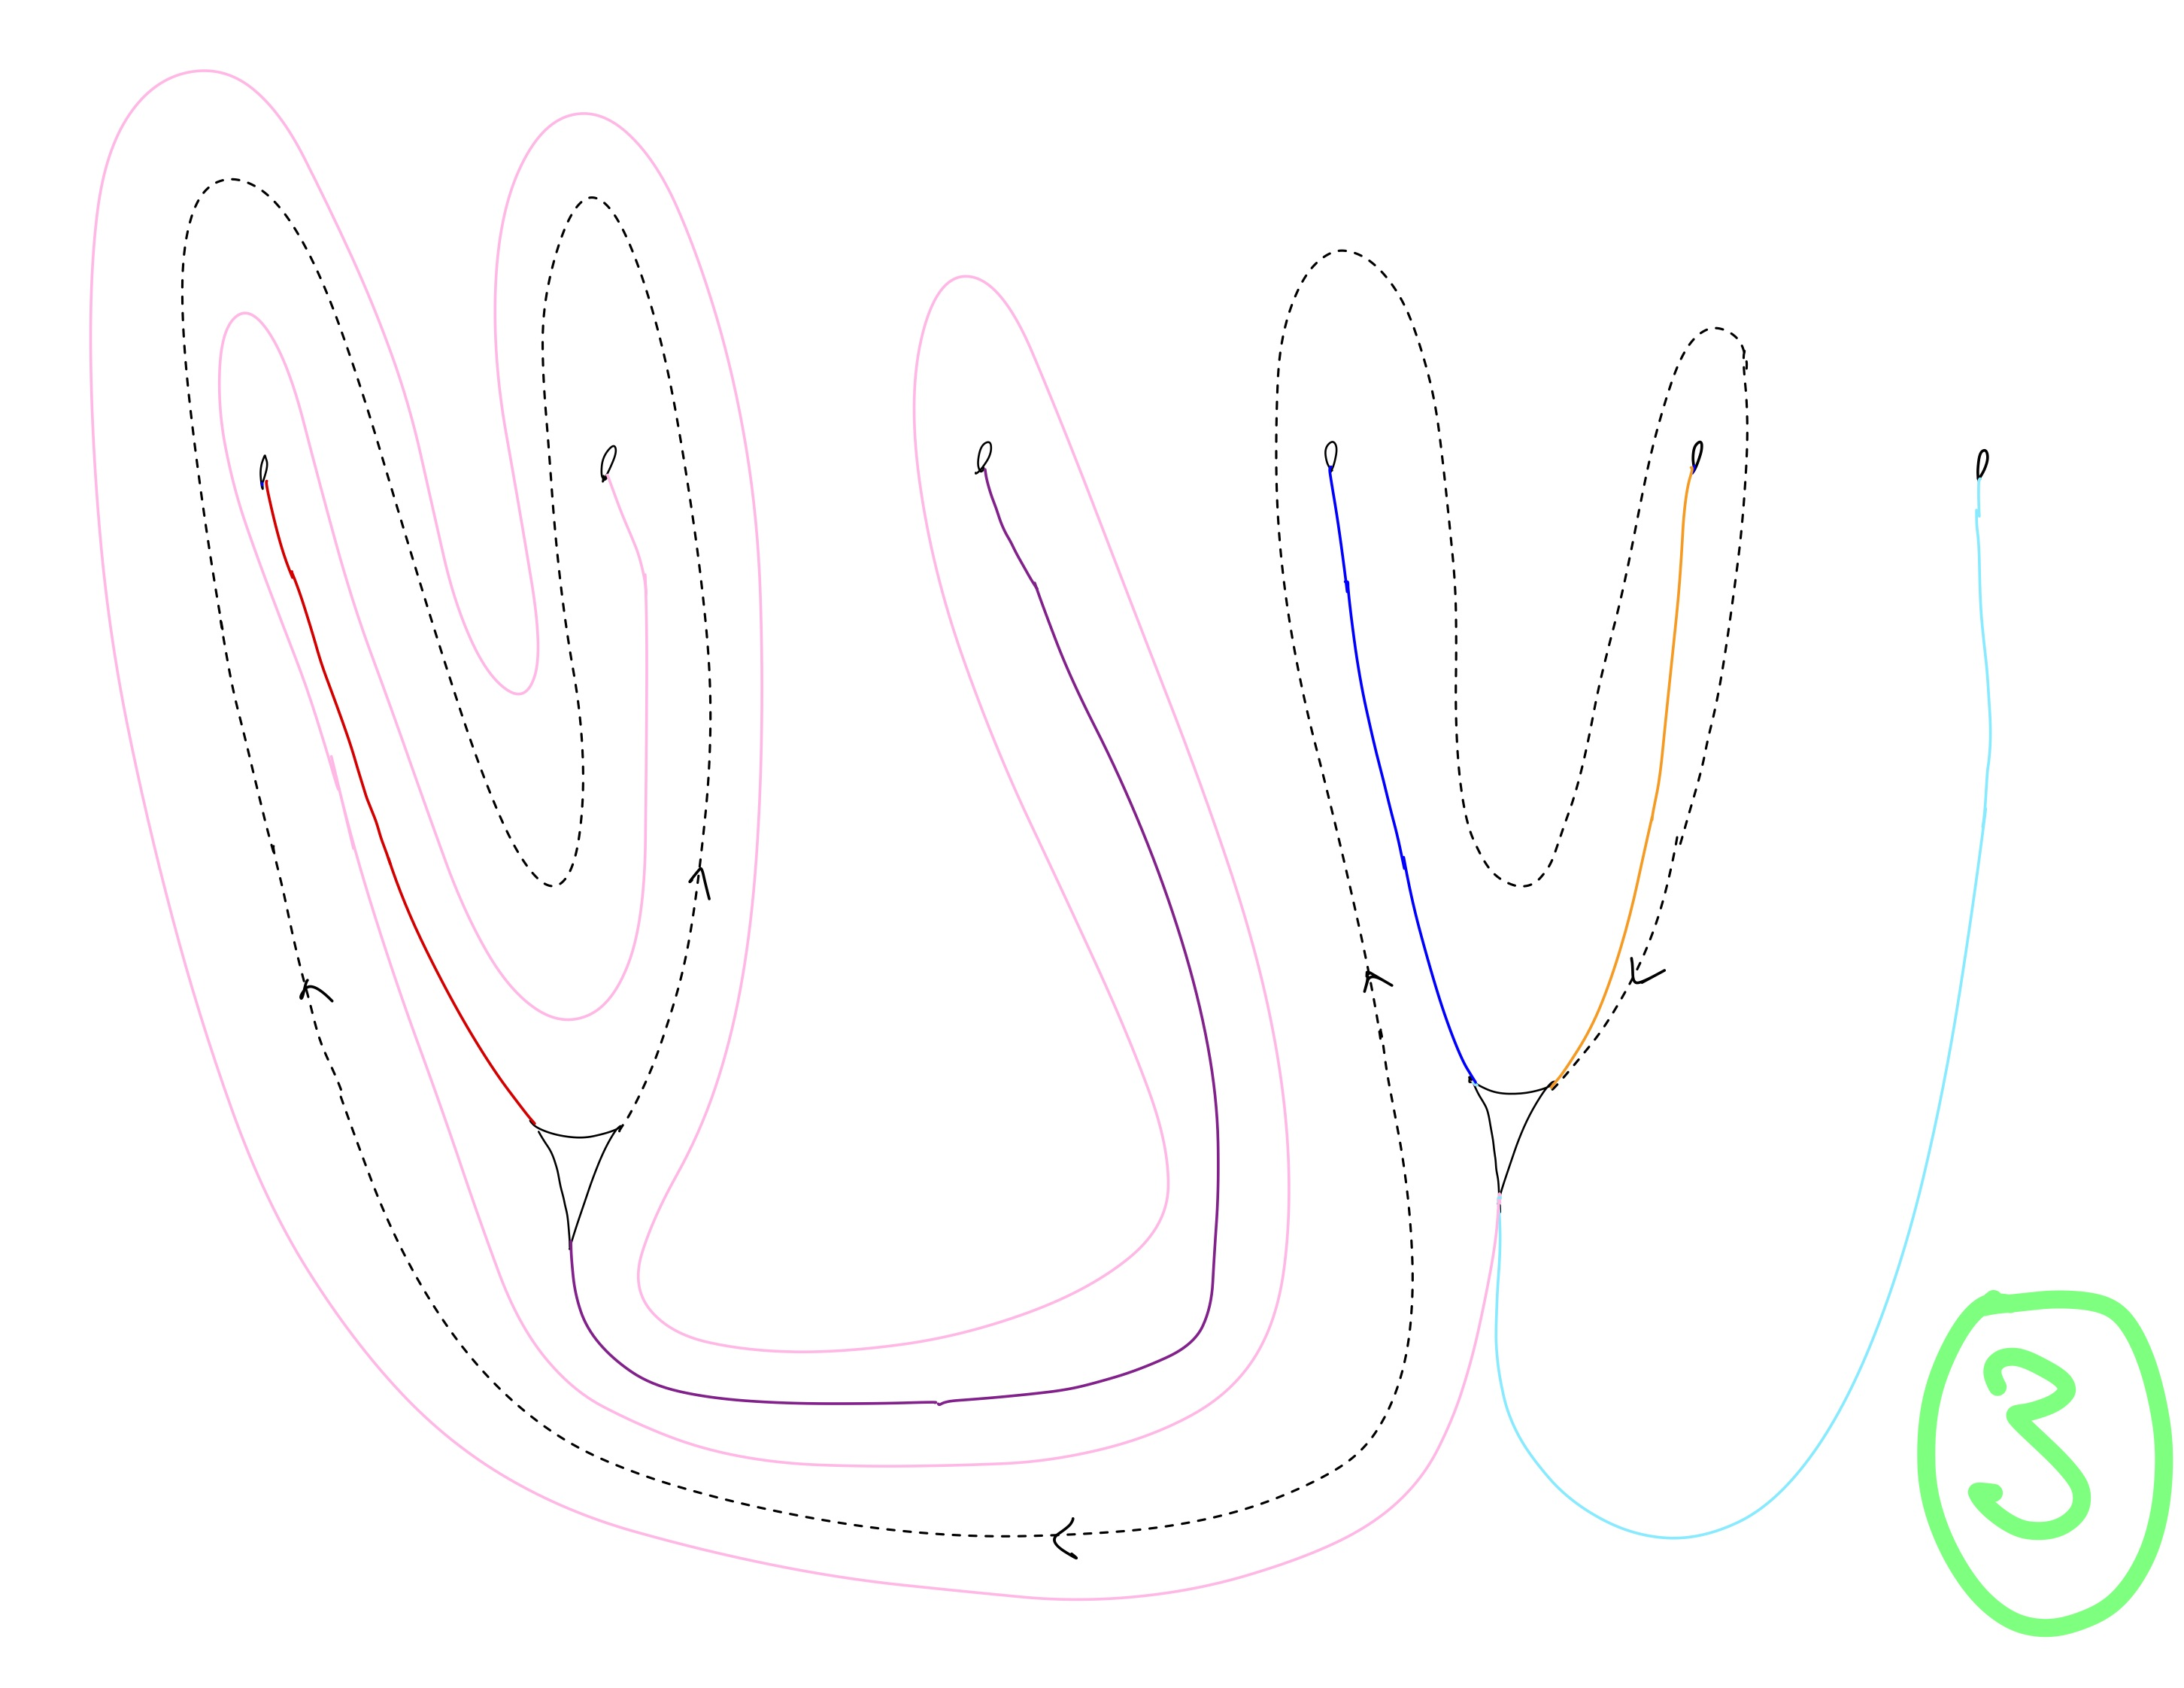
\includegraphics[width=\linewidth, height=0.45\textheight, keepaspectratio]{figures_braid/figures_track_17/Track 17 Braid 3 Wanion-1.jpg}
    \caption{Train Track Map Candidate Family 3 (Wanion) of Track 17.}
    \label{fig:track17_braid_b17_3_map}
\end{figure*}

The inverse of the following braid carries this family of train track maps:
\[
b_3^{17} = \sigma_{1} \sigma_{1} \sigma_{2} \sigma_{2} \sigma_{1} \sigma_{2} \sigma_{5} \sigma_{4} \sigma_{5} \sigma_{5} \sigma_{1} \sigma_{2} \sigma_{3} \sigma_{4} \sigma_{5} \sigma_{5} \sigma_{4}
\]

This is shown in Figure \ref{fig:track17_braid_b17_3}.

\begin{figure*}[p]
    \centering
    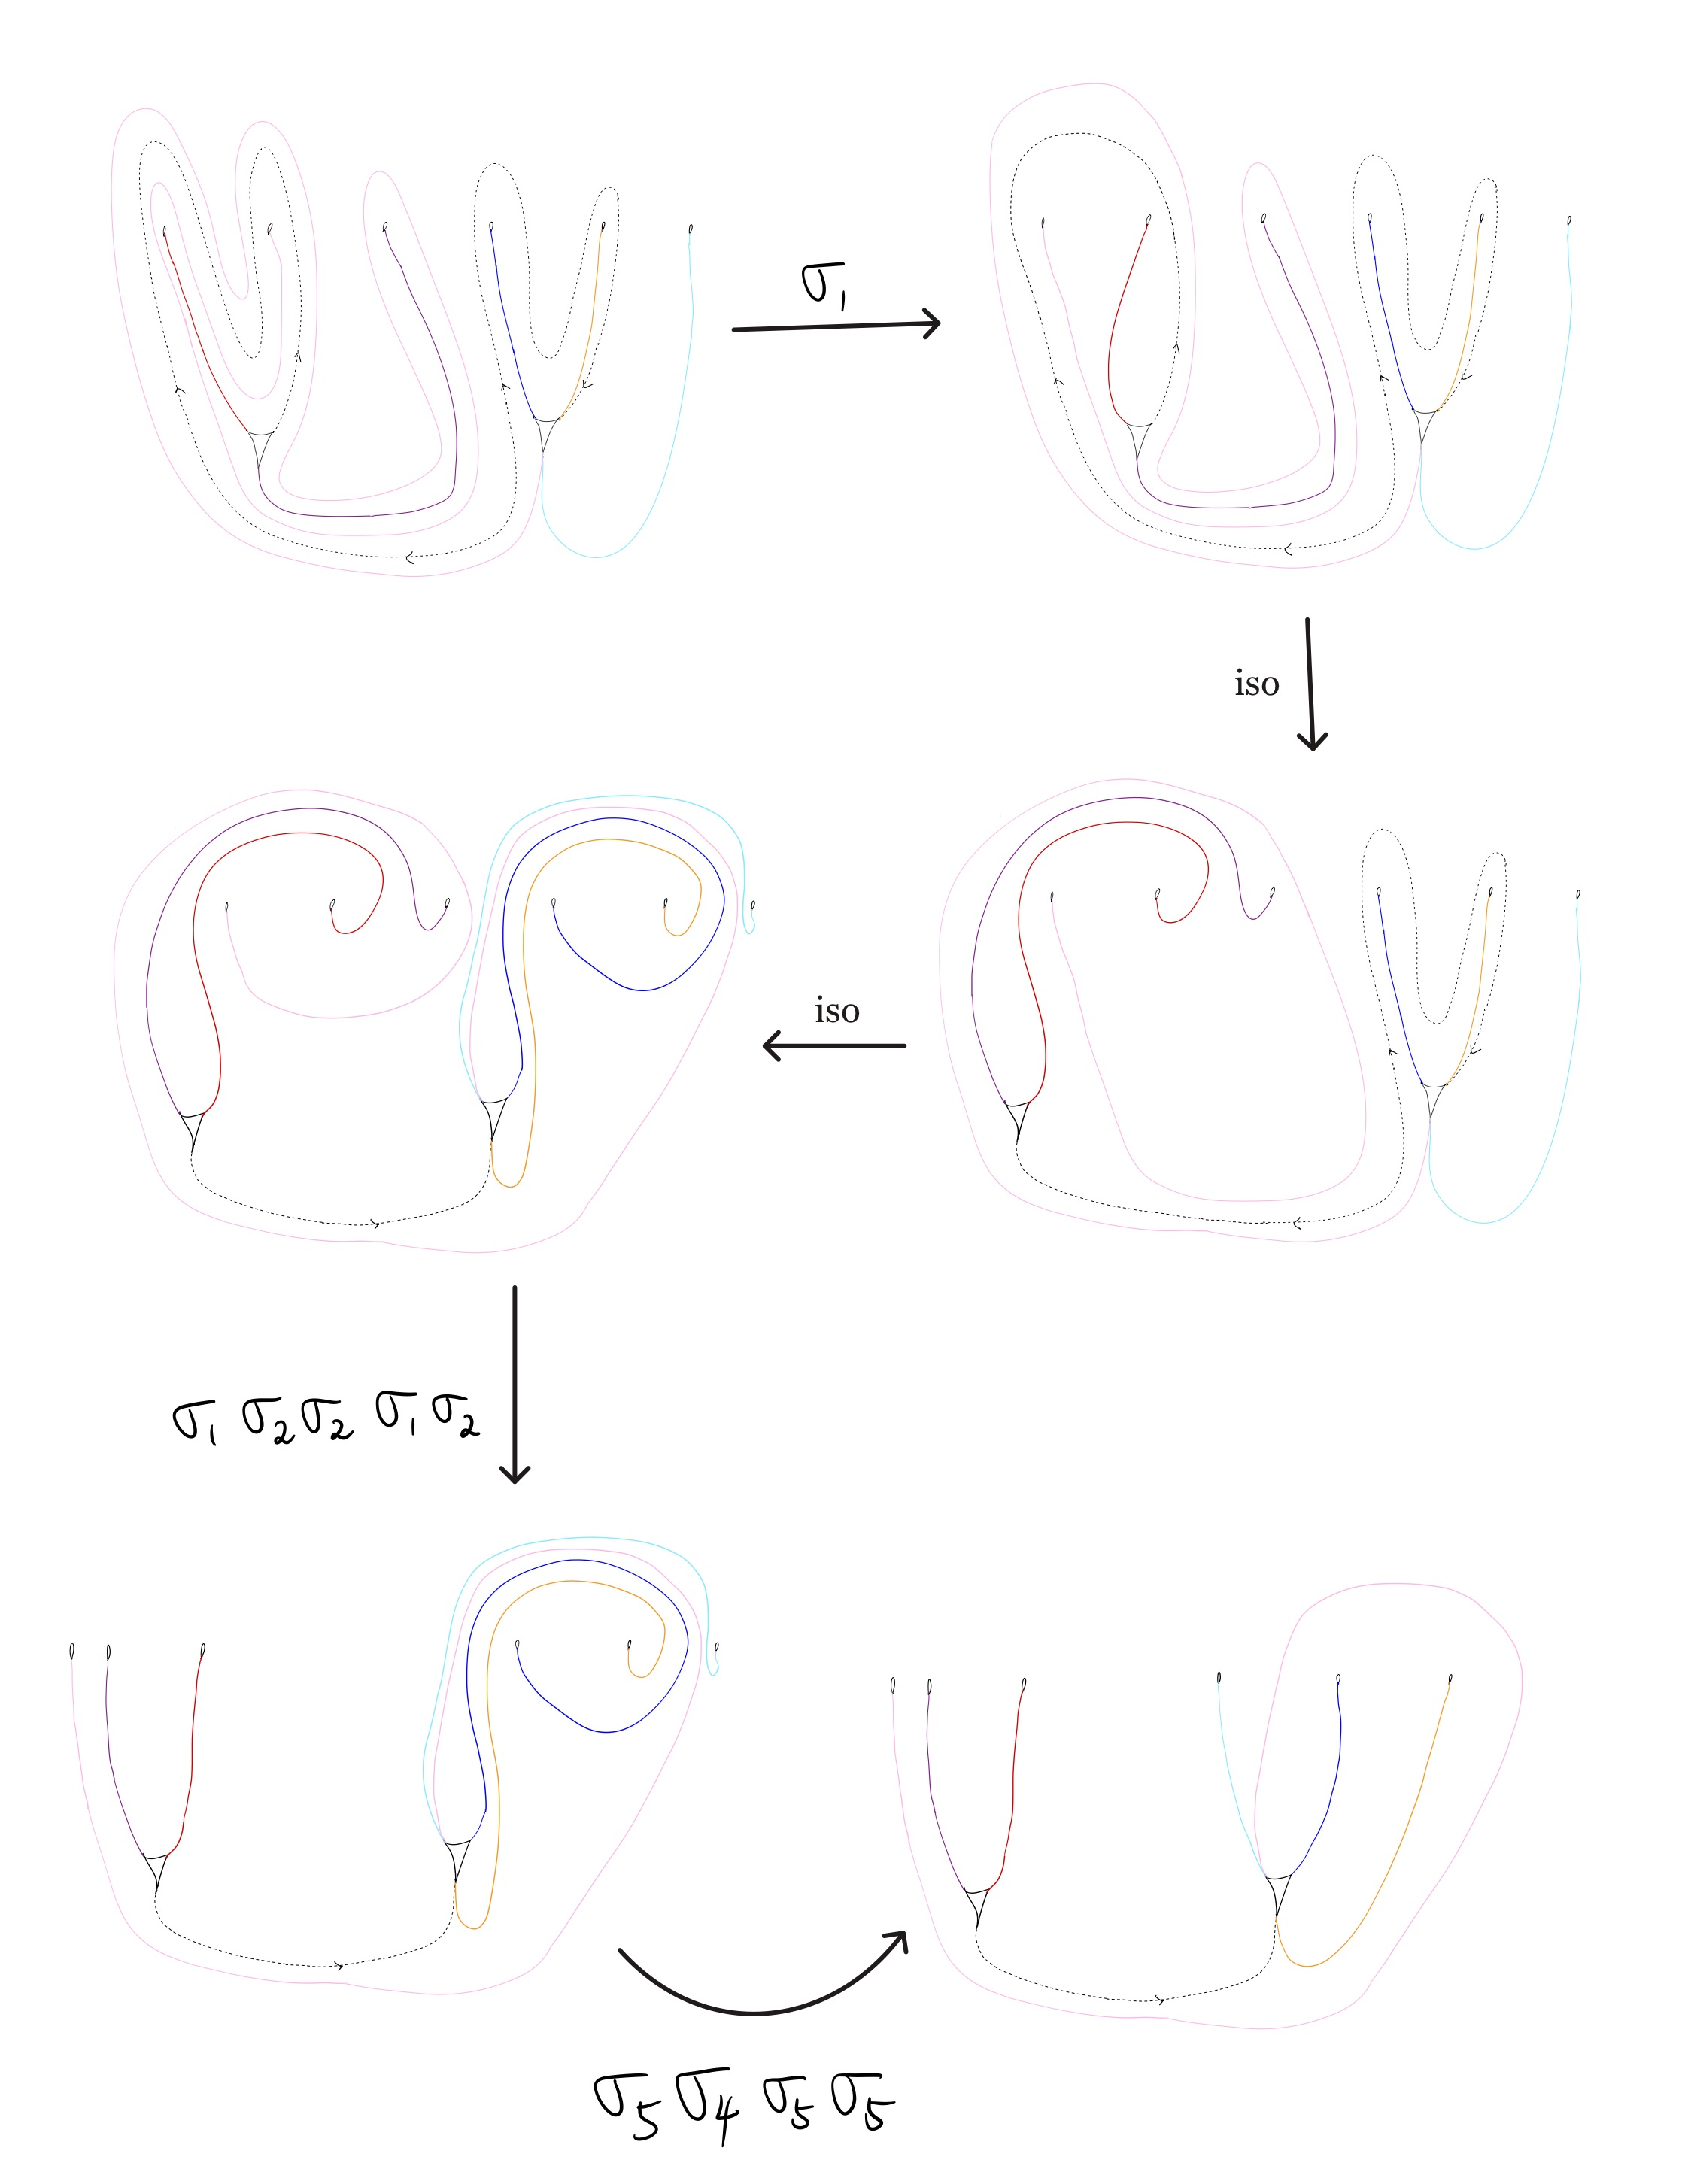
\includegraphics[width=\linewidth, height=0.45\textheight, keepaspectratio]{figures_braid/figures_track_17/Track 17 Braid 3 Wanion-2.jpg}\\
    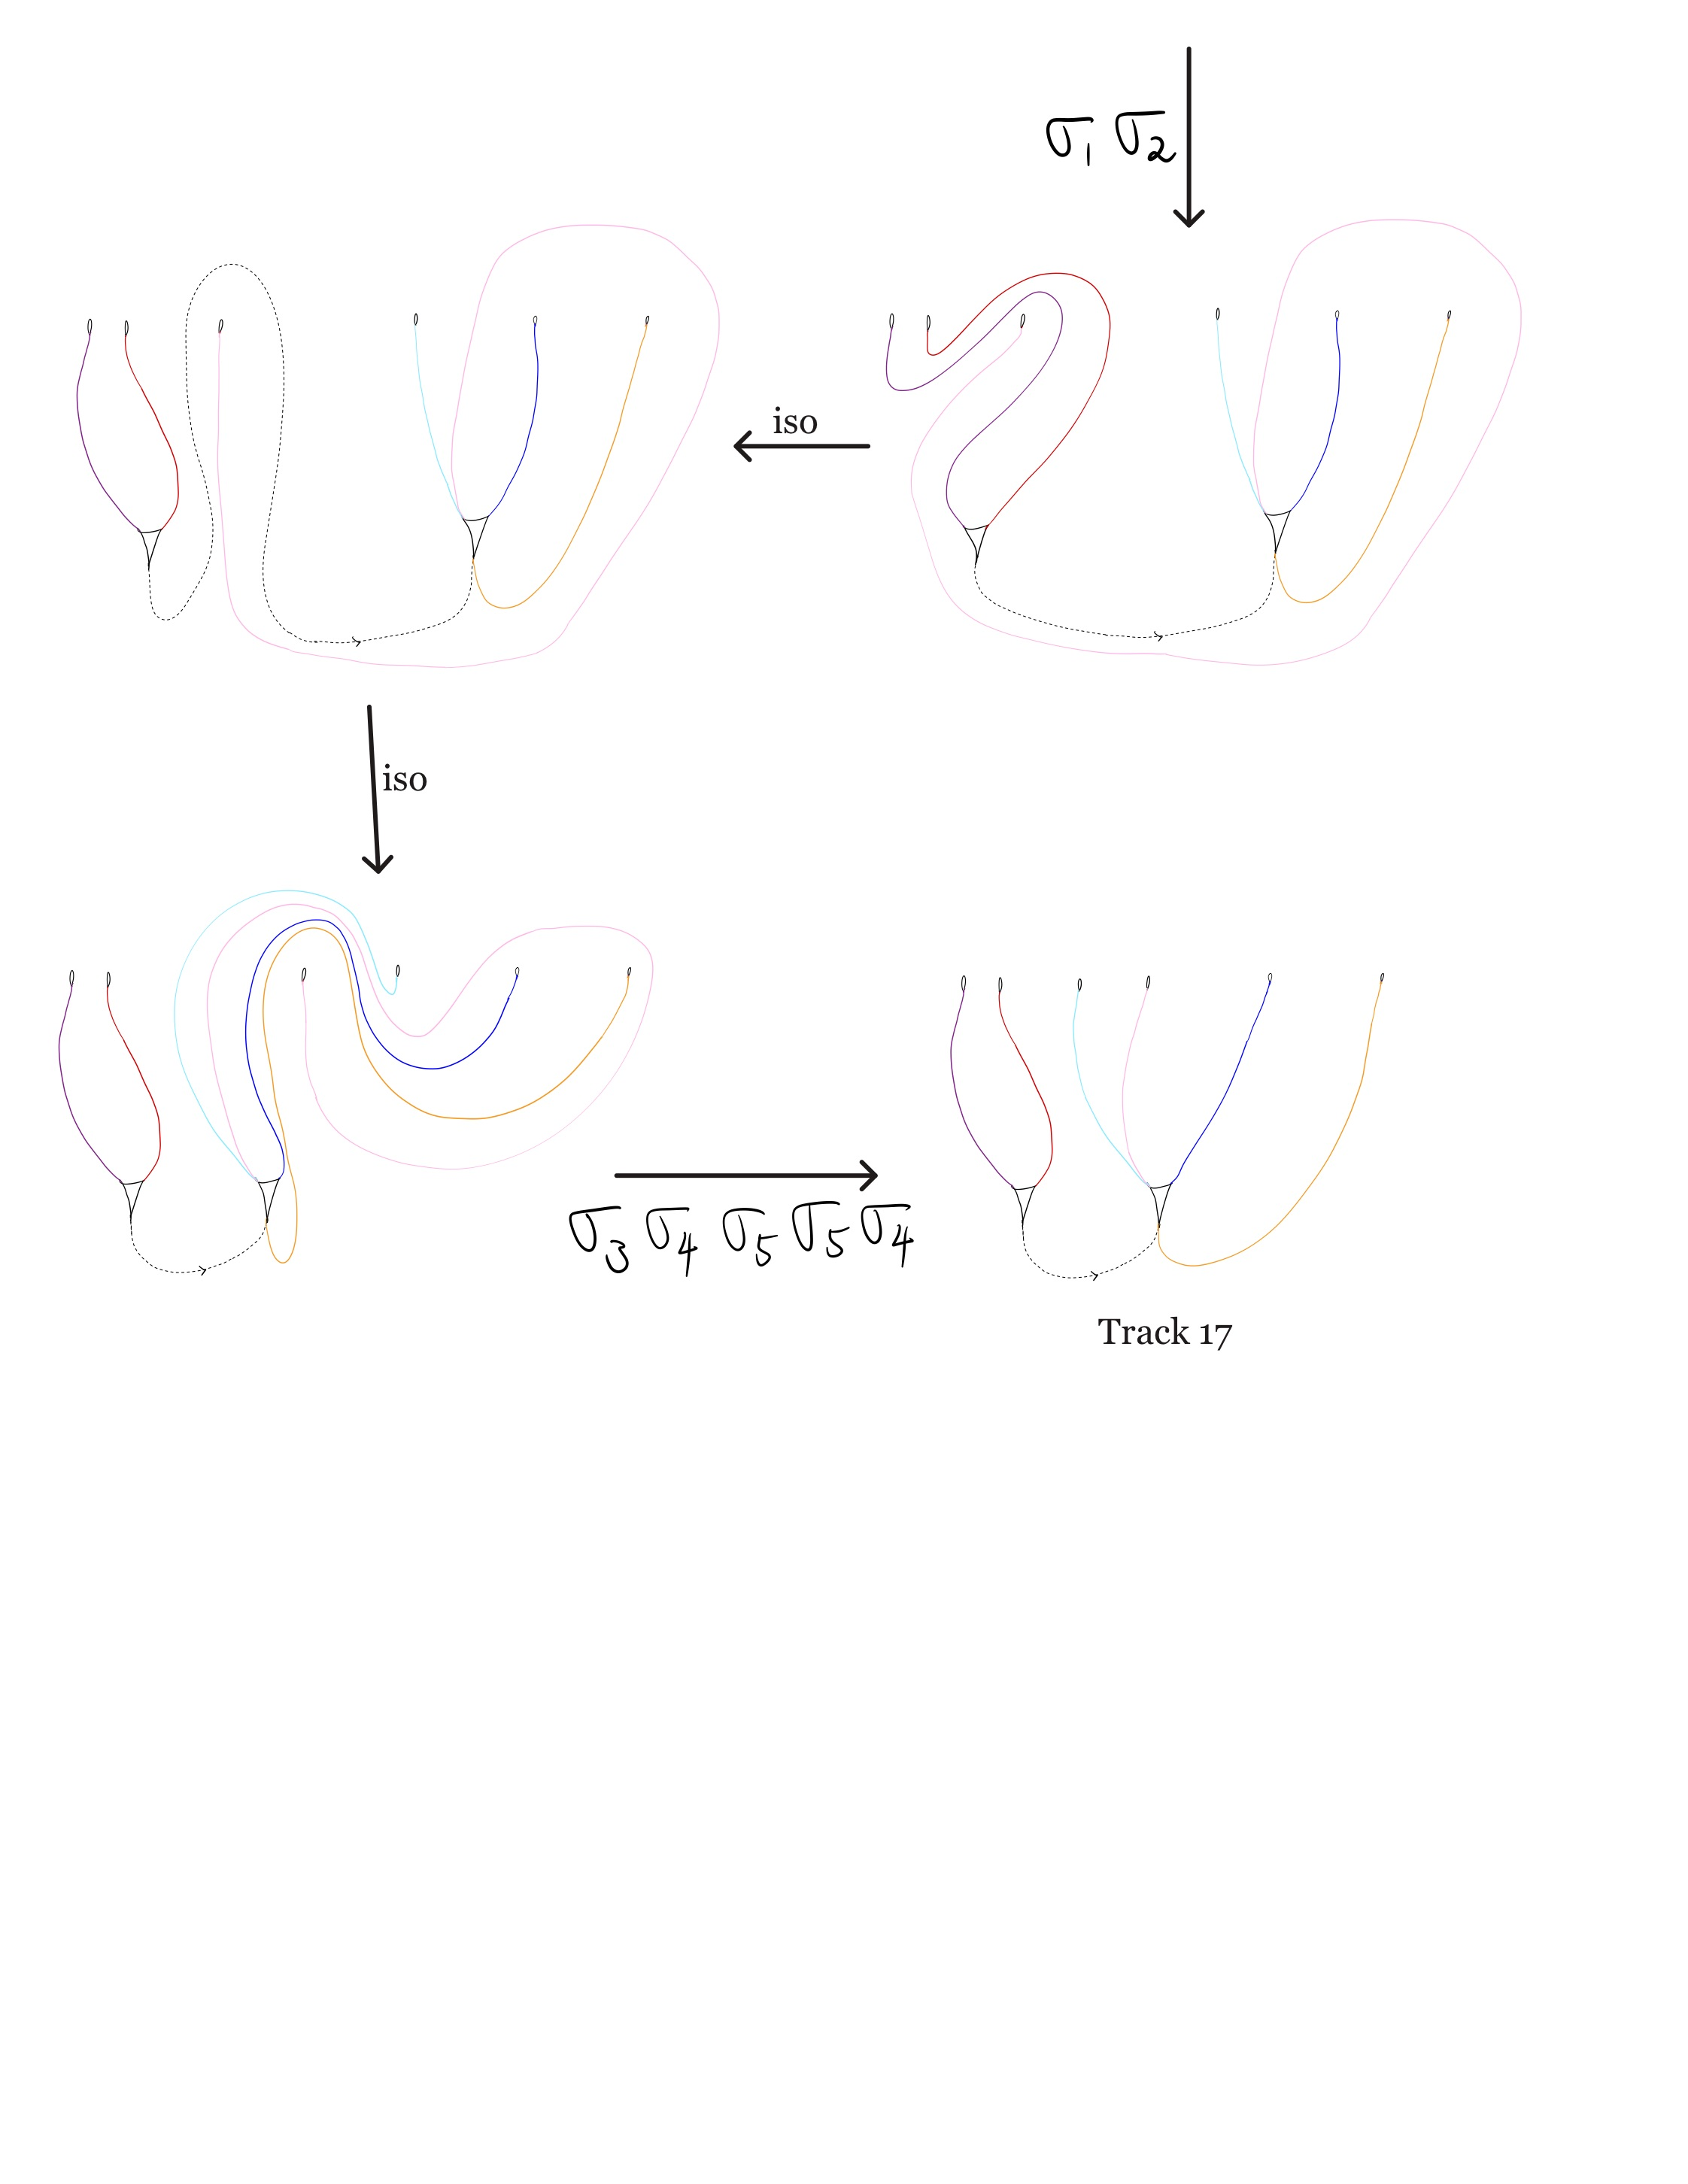
\includegraphics[width=\linewidth, height=0.45\textheight, keepaspectratio]{figures_braid/figures_track_17/Track 17 Braid 3 Wanion-3.jpg}
    \caption{This sequence shows the inverse of the braid $b_3^{17}$ carries Train Track Candidate Family 3.}
    \label{fig:track17_braid_b17_3}
\end{figure*}

\clearpage

\section{Candidate Family 4 (Roop)}\label{sec:track17_roop}
Train Track Map Candidate Family 4 of Track 17 is shown in Figure \ref{fig:track17_braid_b17_4_map}. See \ref{Roop} for details.

\begin{figure*}[ht]
    \centering
    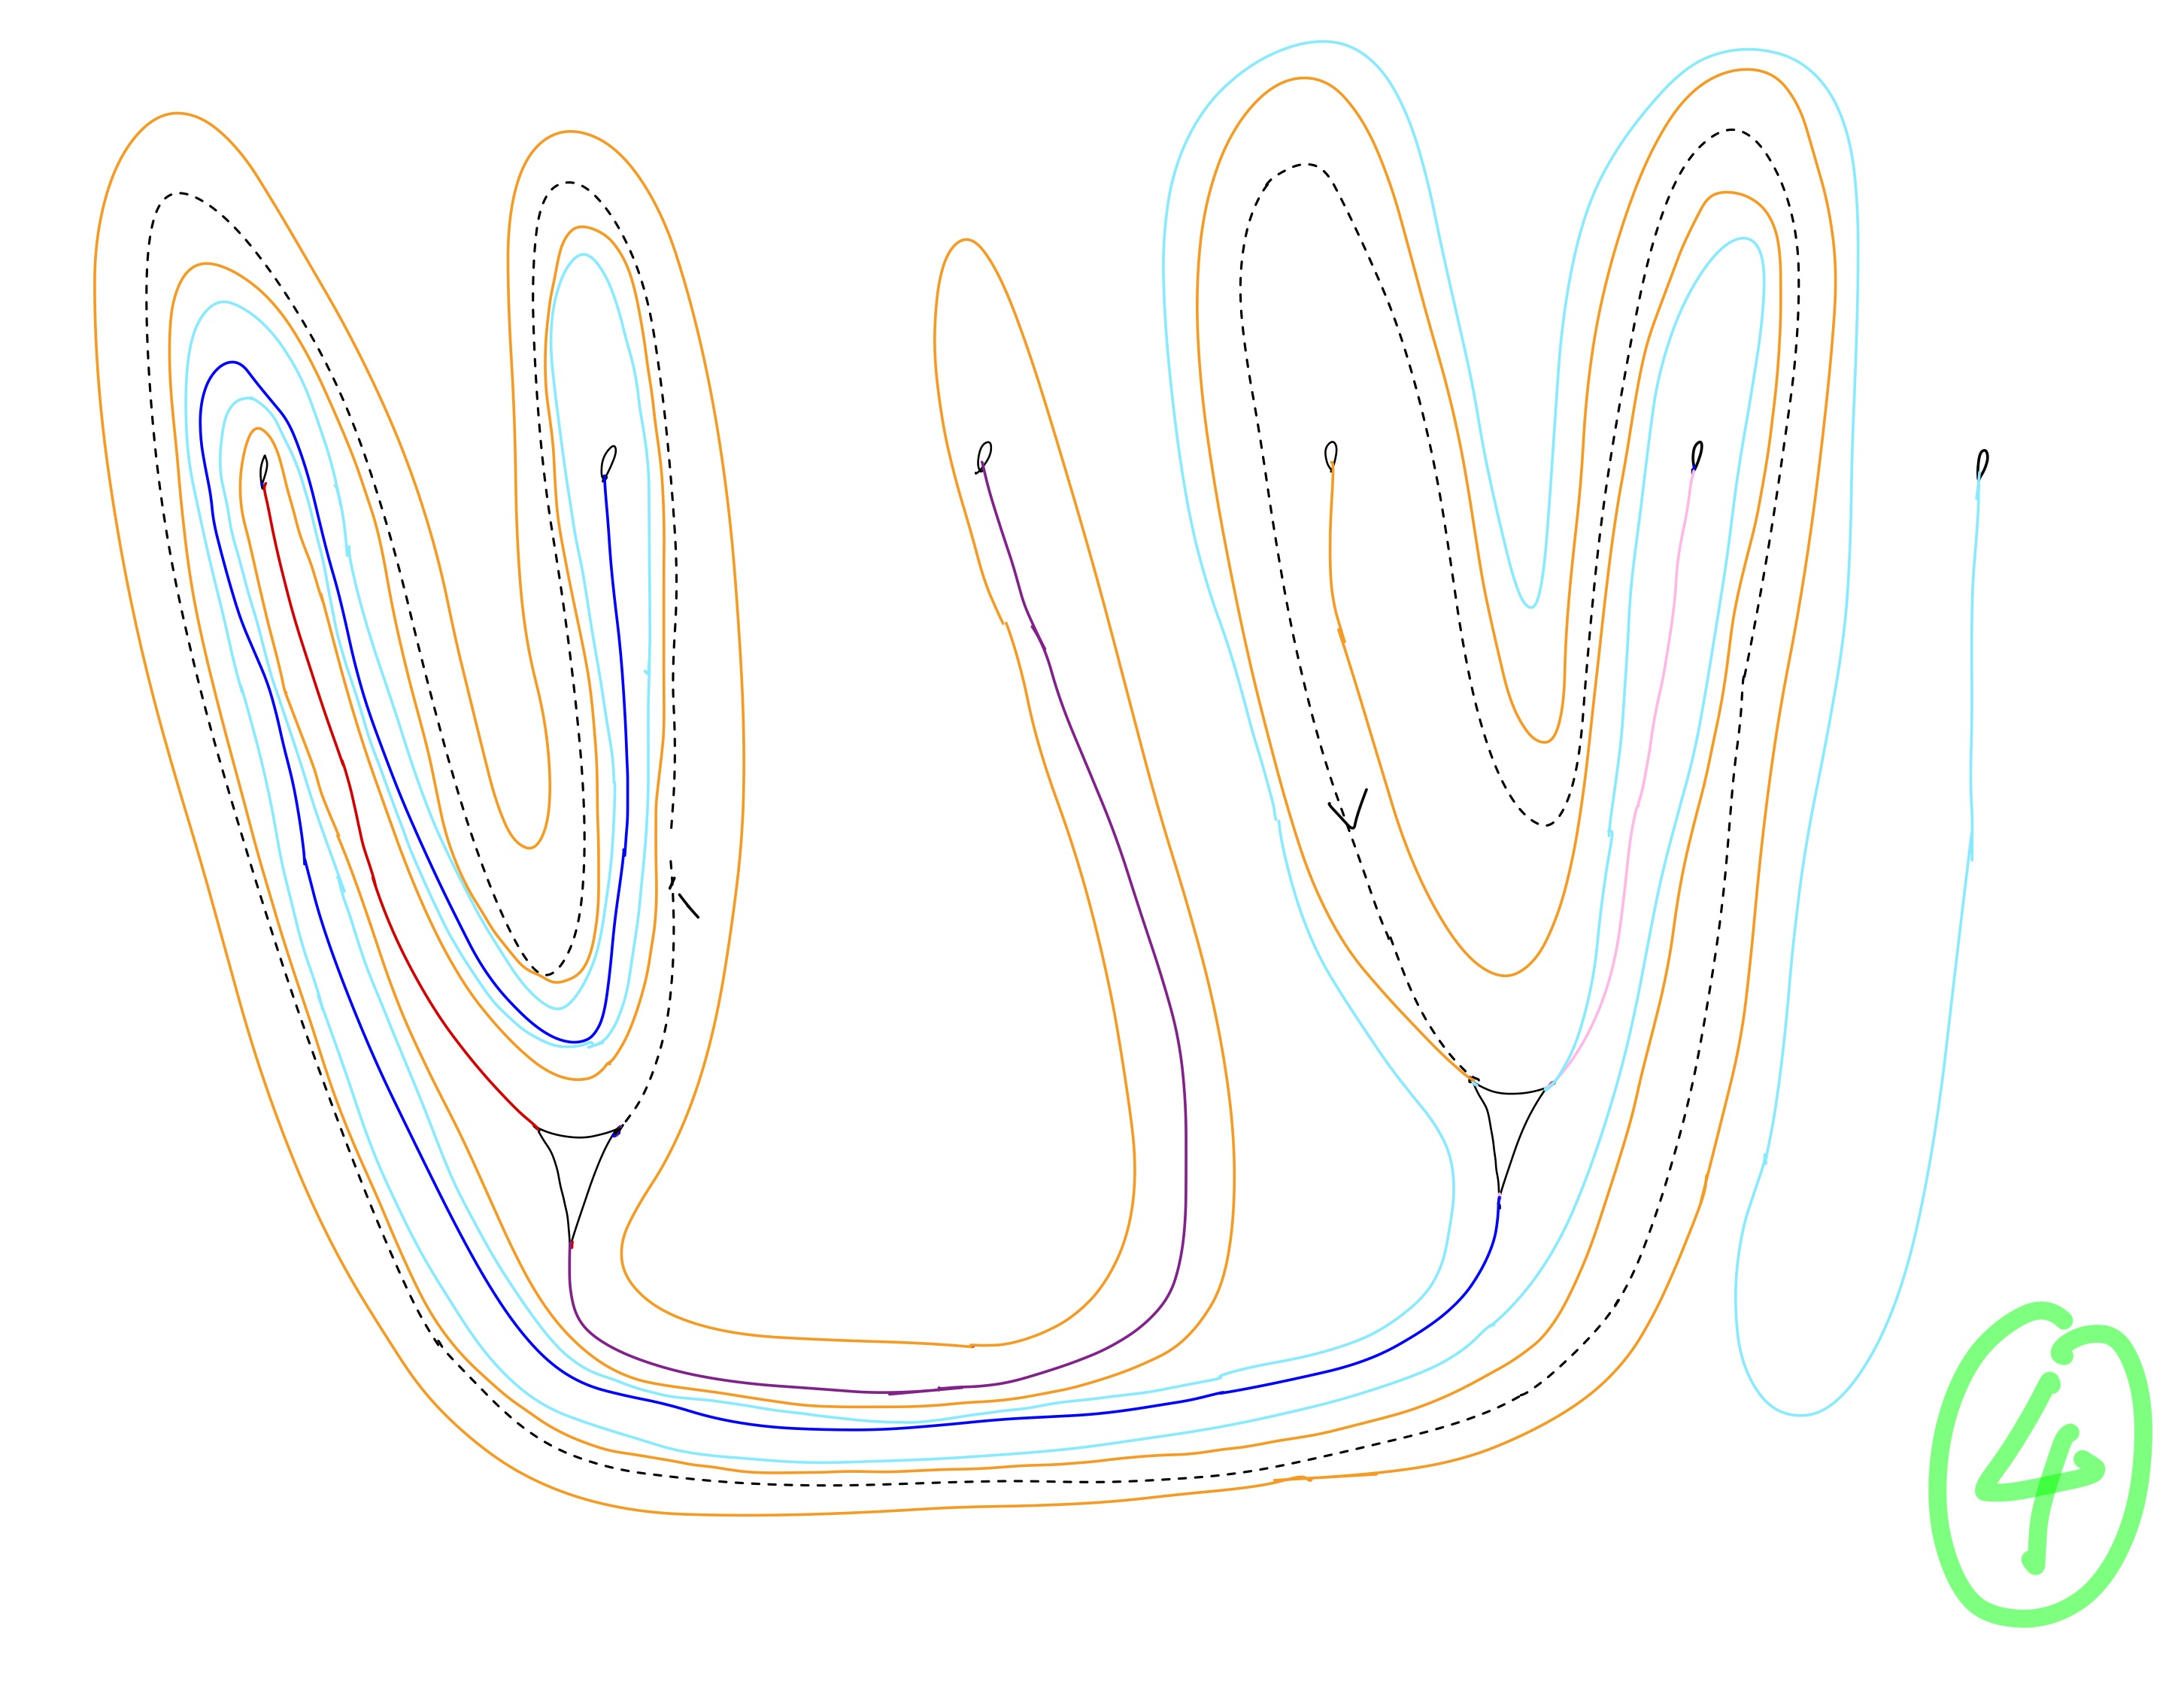
\includegraphics[width=\linewidth, height=0.45\textheight, keepaspectratio]{figures_braid/figures_track_17/Track 17 Braid 4 Roop-1.jpg}
    \caption{Train Track Map Candidate Family 4 (Roop) of Track 17.}
    \label{fig:track17_braid_b17_4_map}
\end{figure*}

The inverse of the following braid carries this family of train track maps:
\[
b_4^{17} = \sigma_{1} \sigma_{5} \sigma_{4} \sigma_{2} \sigma_{1} \sigma_{2} \sigma_{3} \sigma_{5}^{-1} \sigma_{4}^{-1} \sigma_{5}^{-1} \sigma_{4}^{-1} \sigma_{3}^{-1} \sigma_{2} \sigma_{1} \sigma_{1} \sigma_{2} \sigma_{3} \sigma_{4} \sigma_{5}
\]

This is shown in Figure \ref{fig:track17_braid_b17_4}.

\begin{figure*}[p]
    \centering
    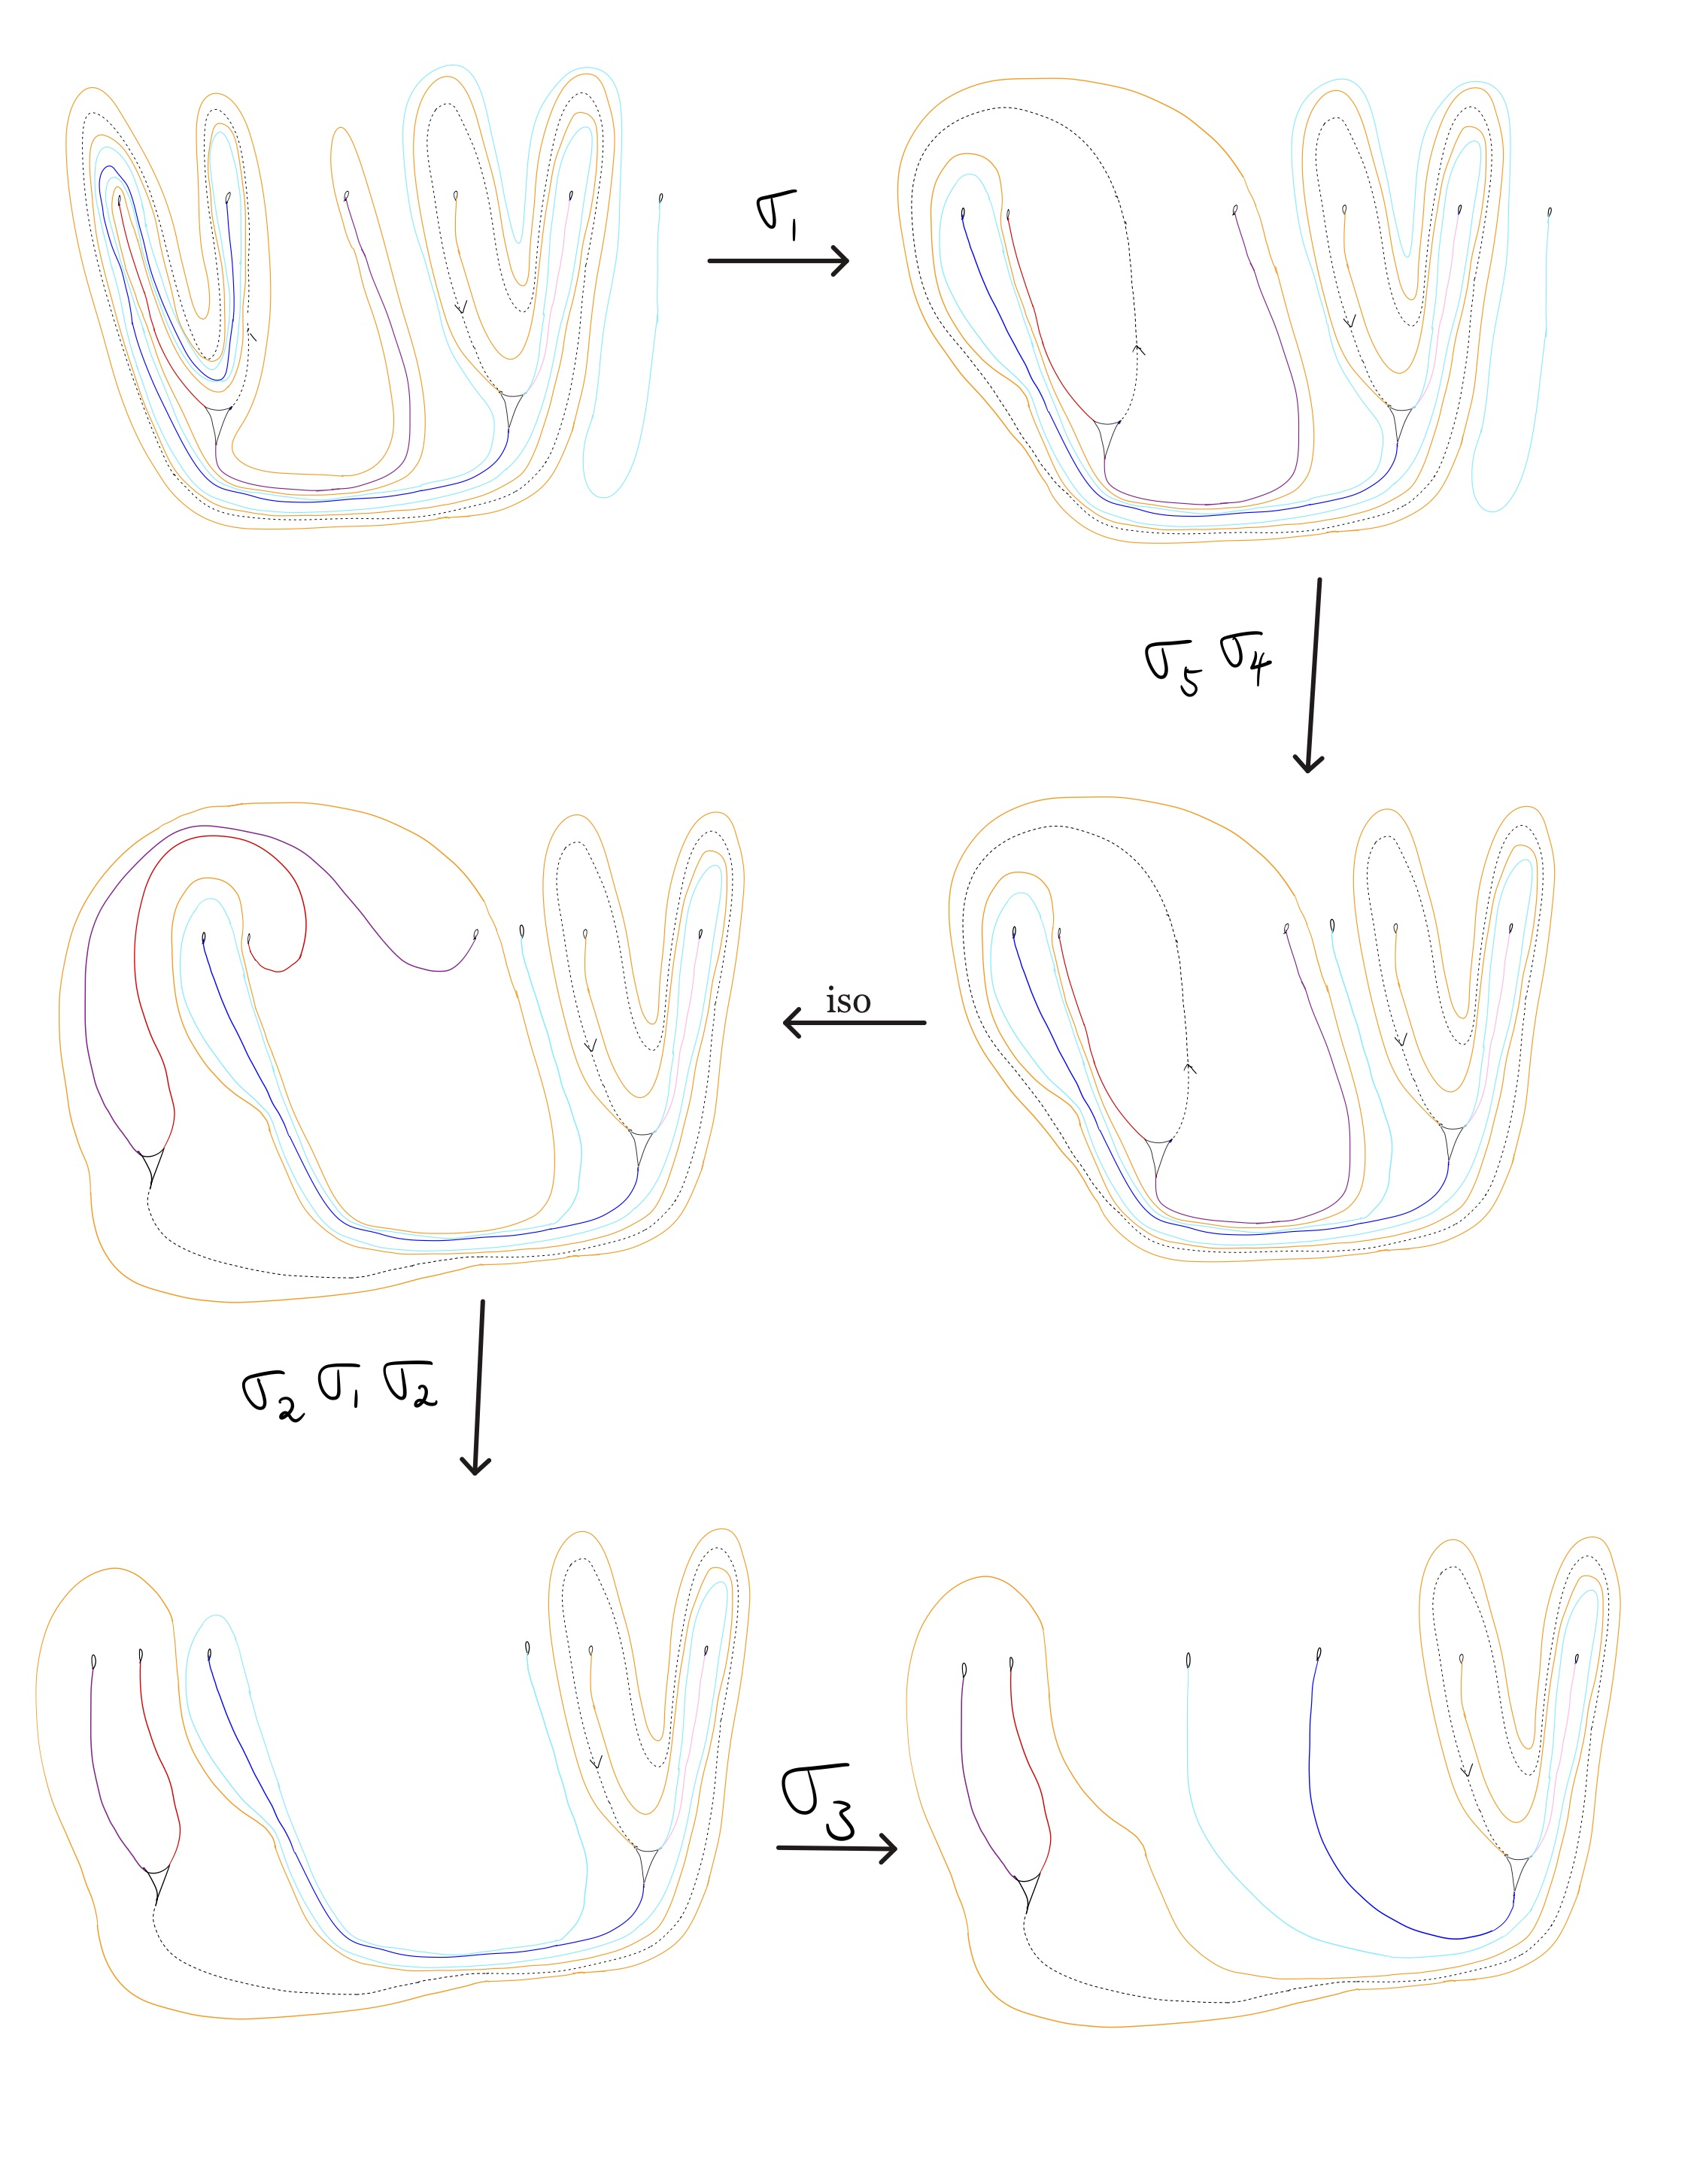
\includegraphics[width=\linewidth, height=0.45\textheight, keepaspectratio]{figures_braid/figures_track_17/Track 17 Braid 4 Roop-2.jpg}\\
    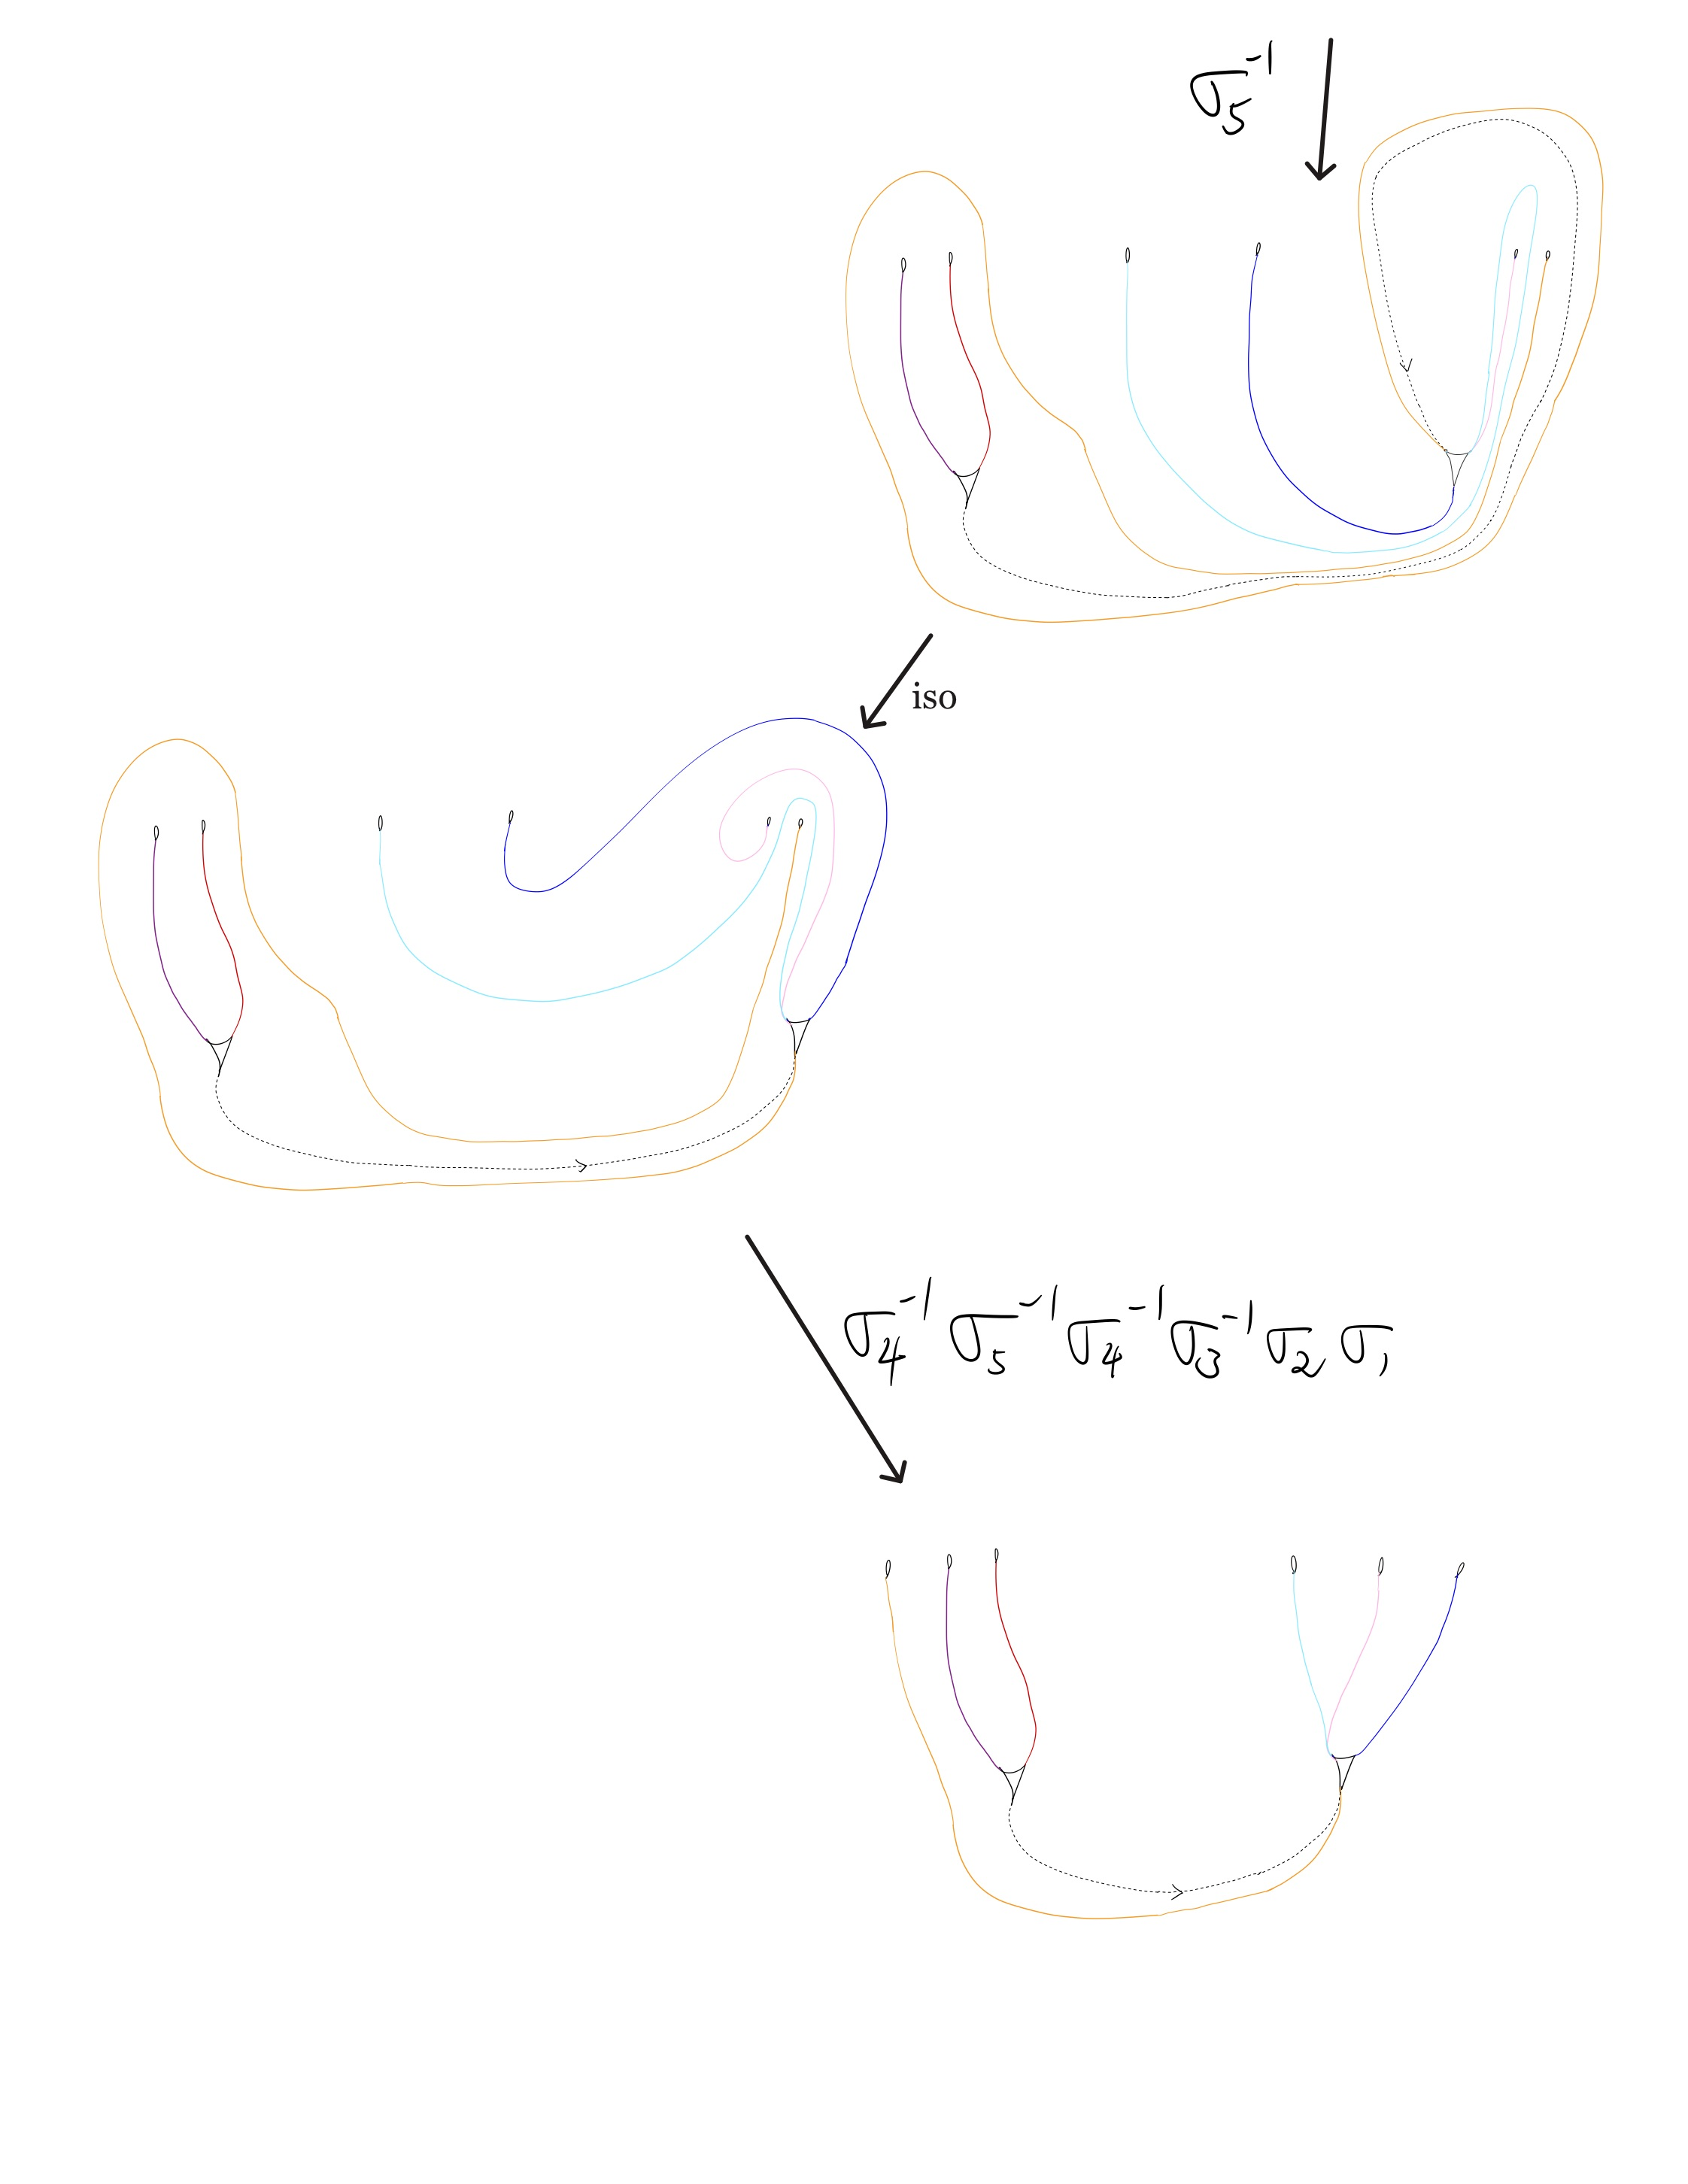
\includegraphics[width=\linewidth, height=0.45\textheight, keepaspectratio]{figures_braid/figures_track_17/Track 17 Braid 4 Roop-3.jpg}
    \caption{This sequence shows the inverse of the braid $b_4^{17}$ carries Train Track Candidate Family 4 (first half).}
    \label{fig:track17_braid_b17_4}
\end{figure*}

\begin{figure*}[p]
    \centering
    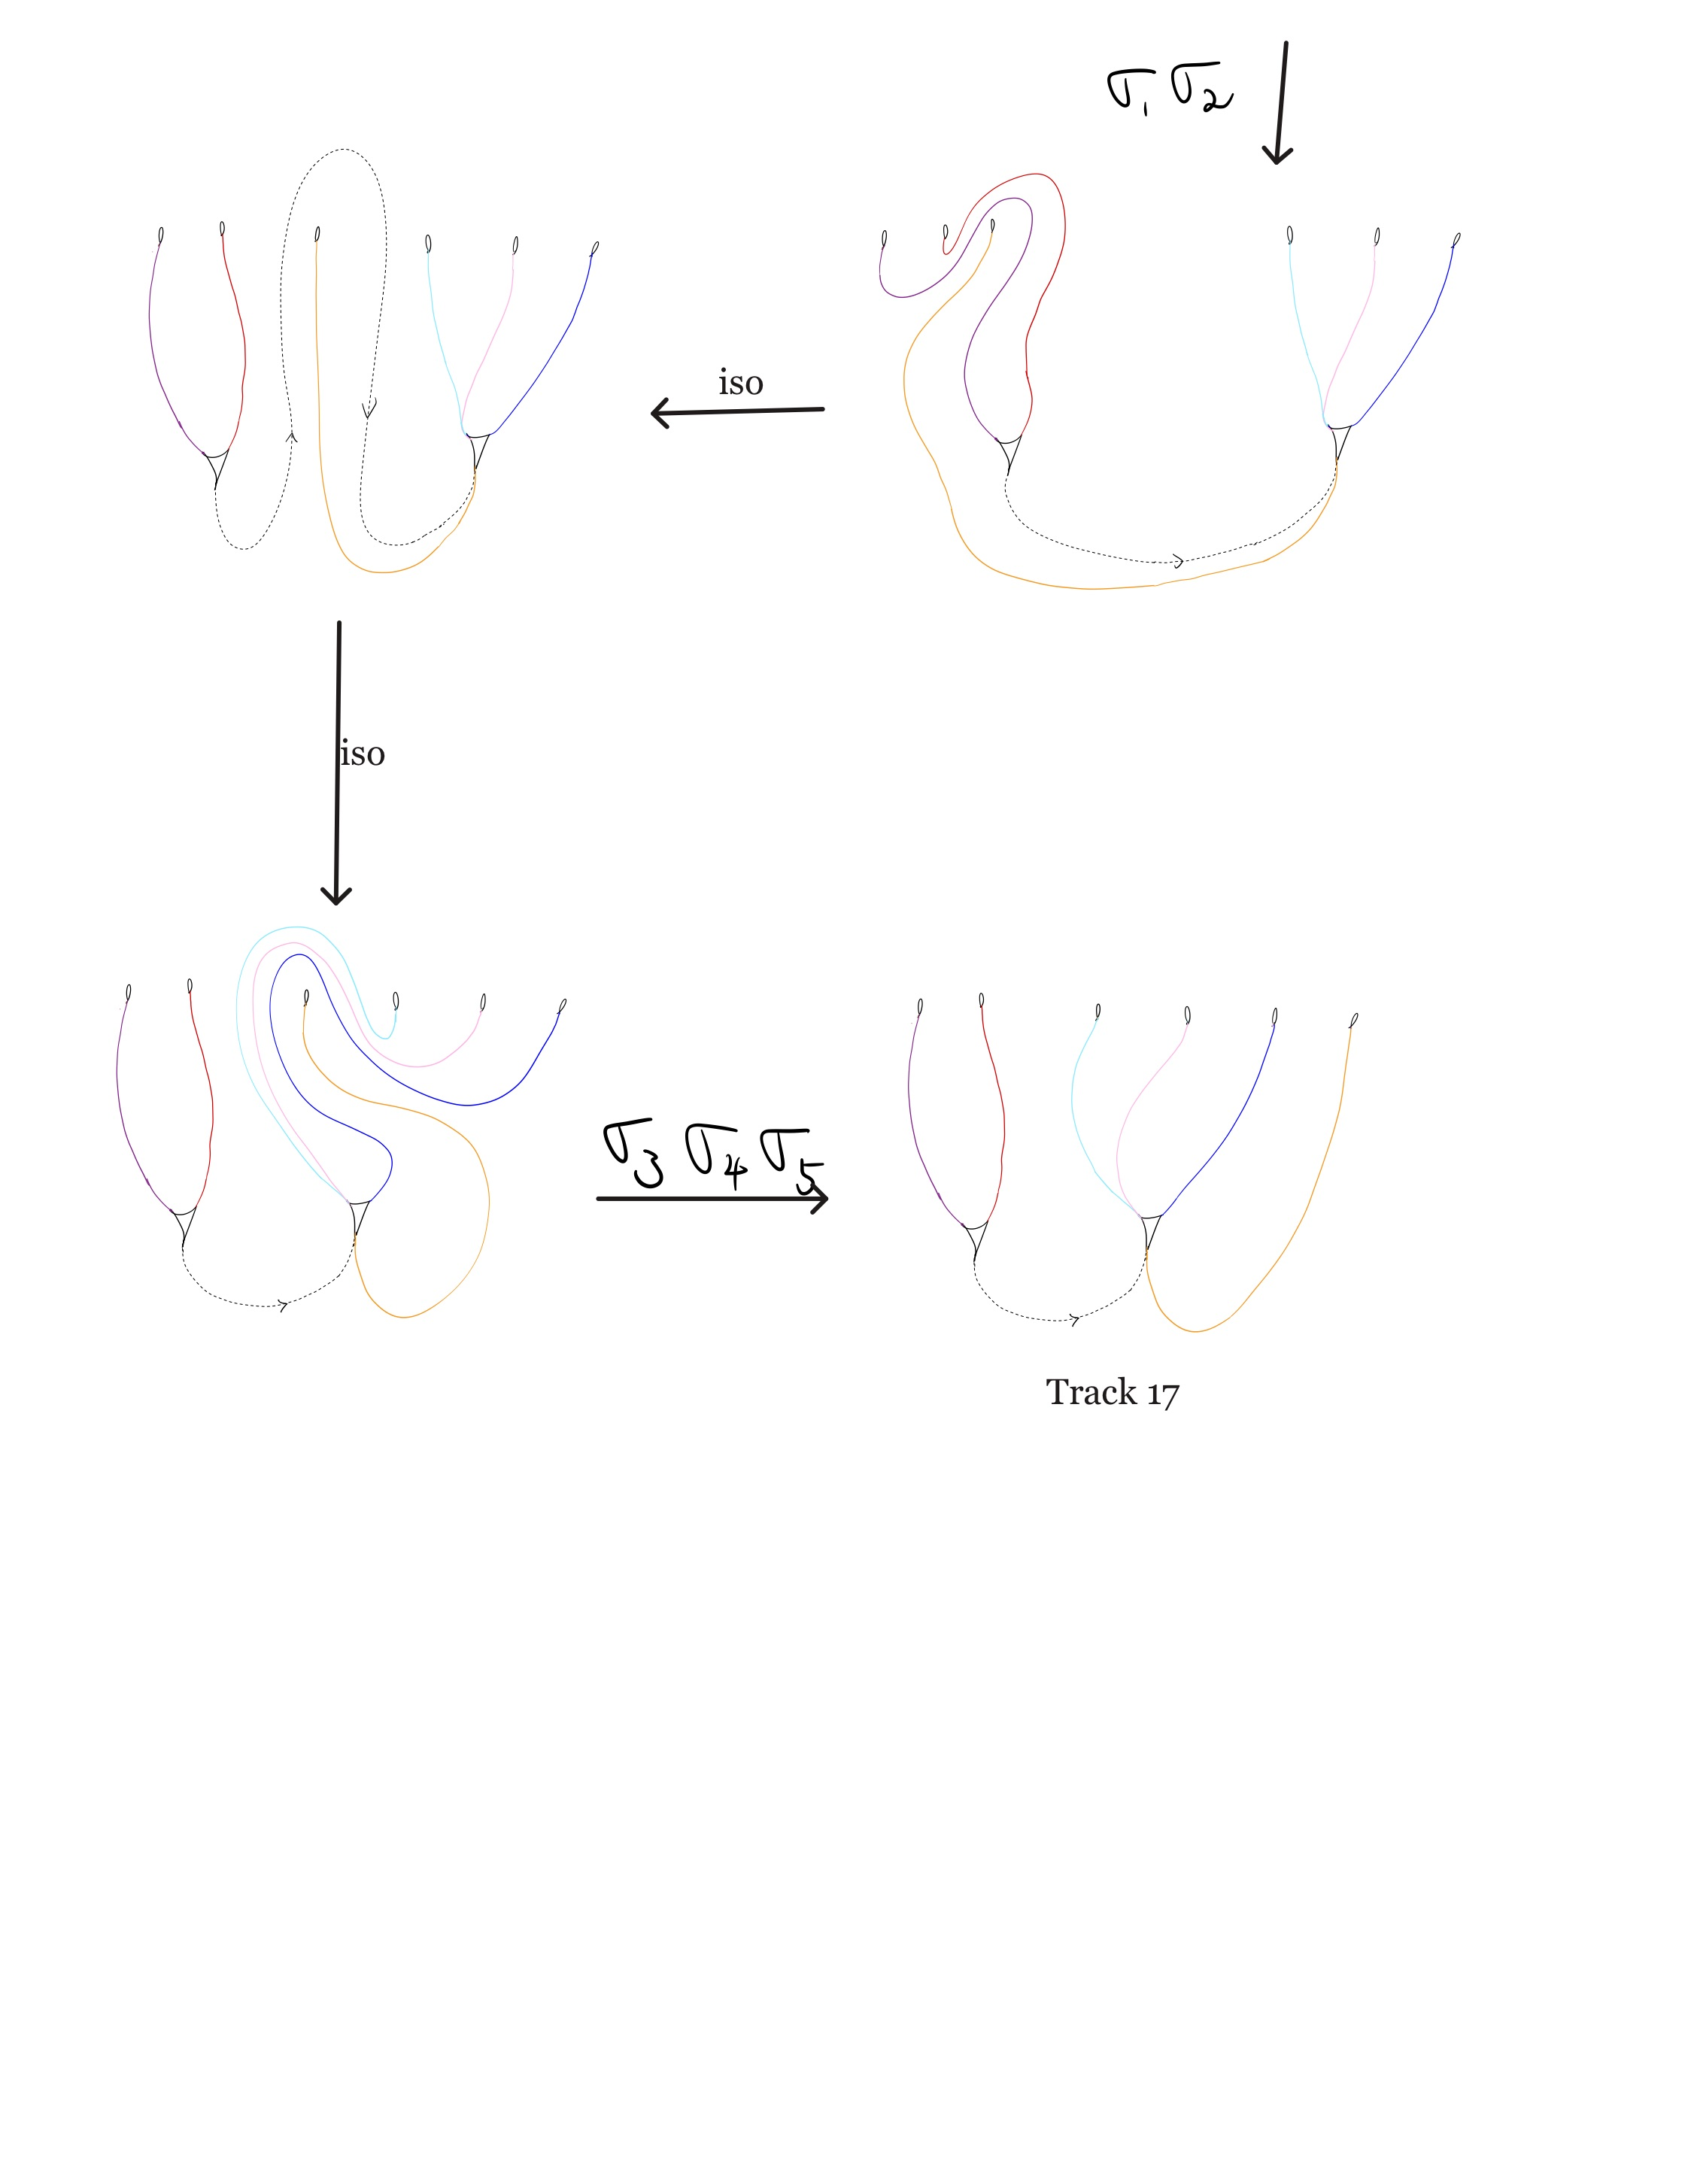
\includegraphics[width=\linewidth, height=0.45\textheight, keepaspectratio]{figures_braid/figures_track_17/Track 17 Braid 4 Roop-4.jpg}
    \caption{Continuation of Figure \ref{fig:track17_braid_b17_4}: the inverse of $b_4^{17}$ carries Train Track Candidate Family 4 (second half).}
    \label{fig:track17_braid_b17_4_cont}
\end{figure*}

\clearpage

\section{Candidate Family 5 (Boke)}\label{sec:track17_boke_5}
Train Track Map Candidate Family 5 of Track 17 is shown in Figure \ref{fig:track17_braid_b17_5_map}. See Section \ref{Boke} for details. This is a parametric family indexed by an integer twist parameter $k \in \mathbb{Z}_{\geq 0}$.

\begin{figure*}[ht]
    \centering
    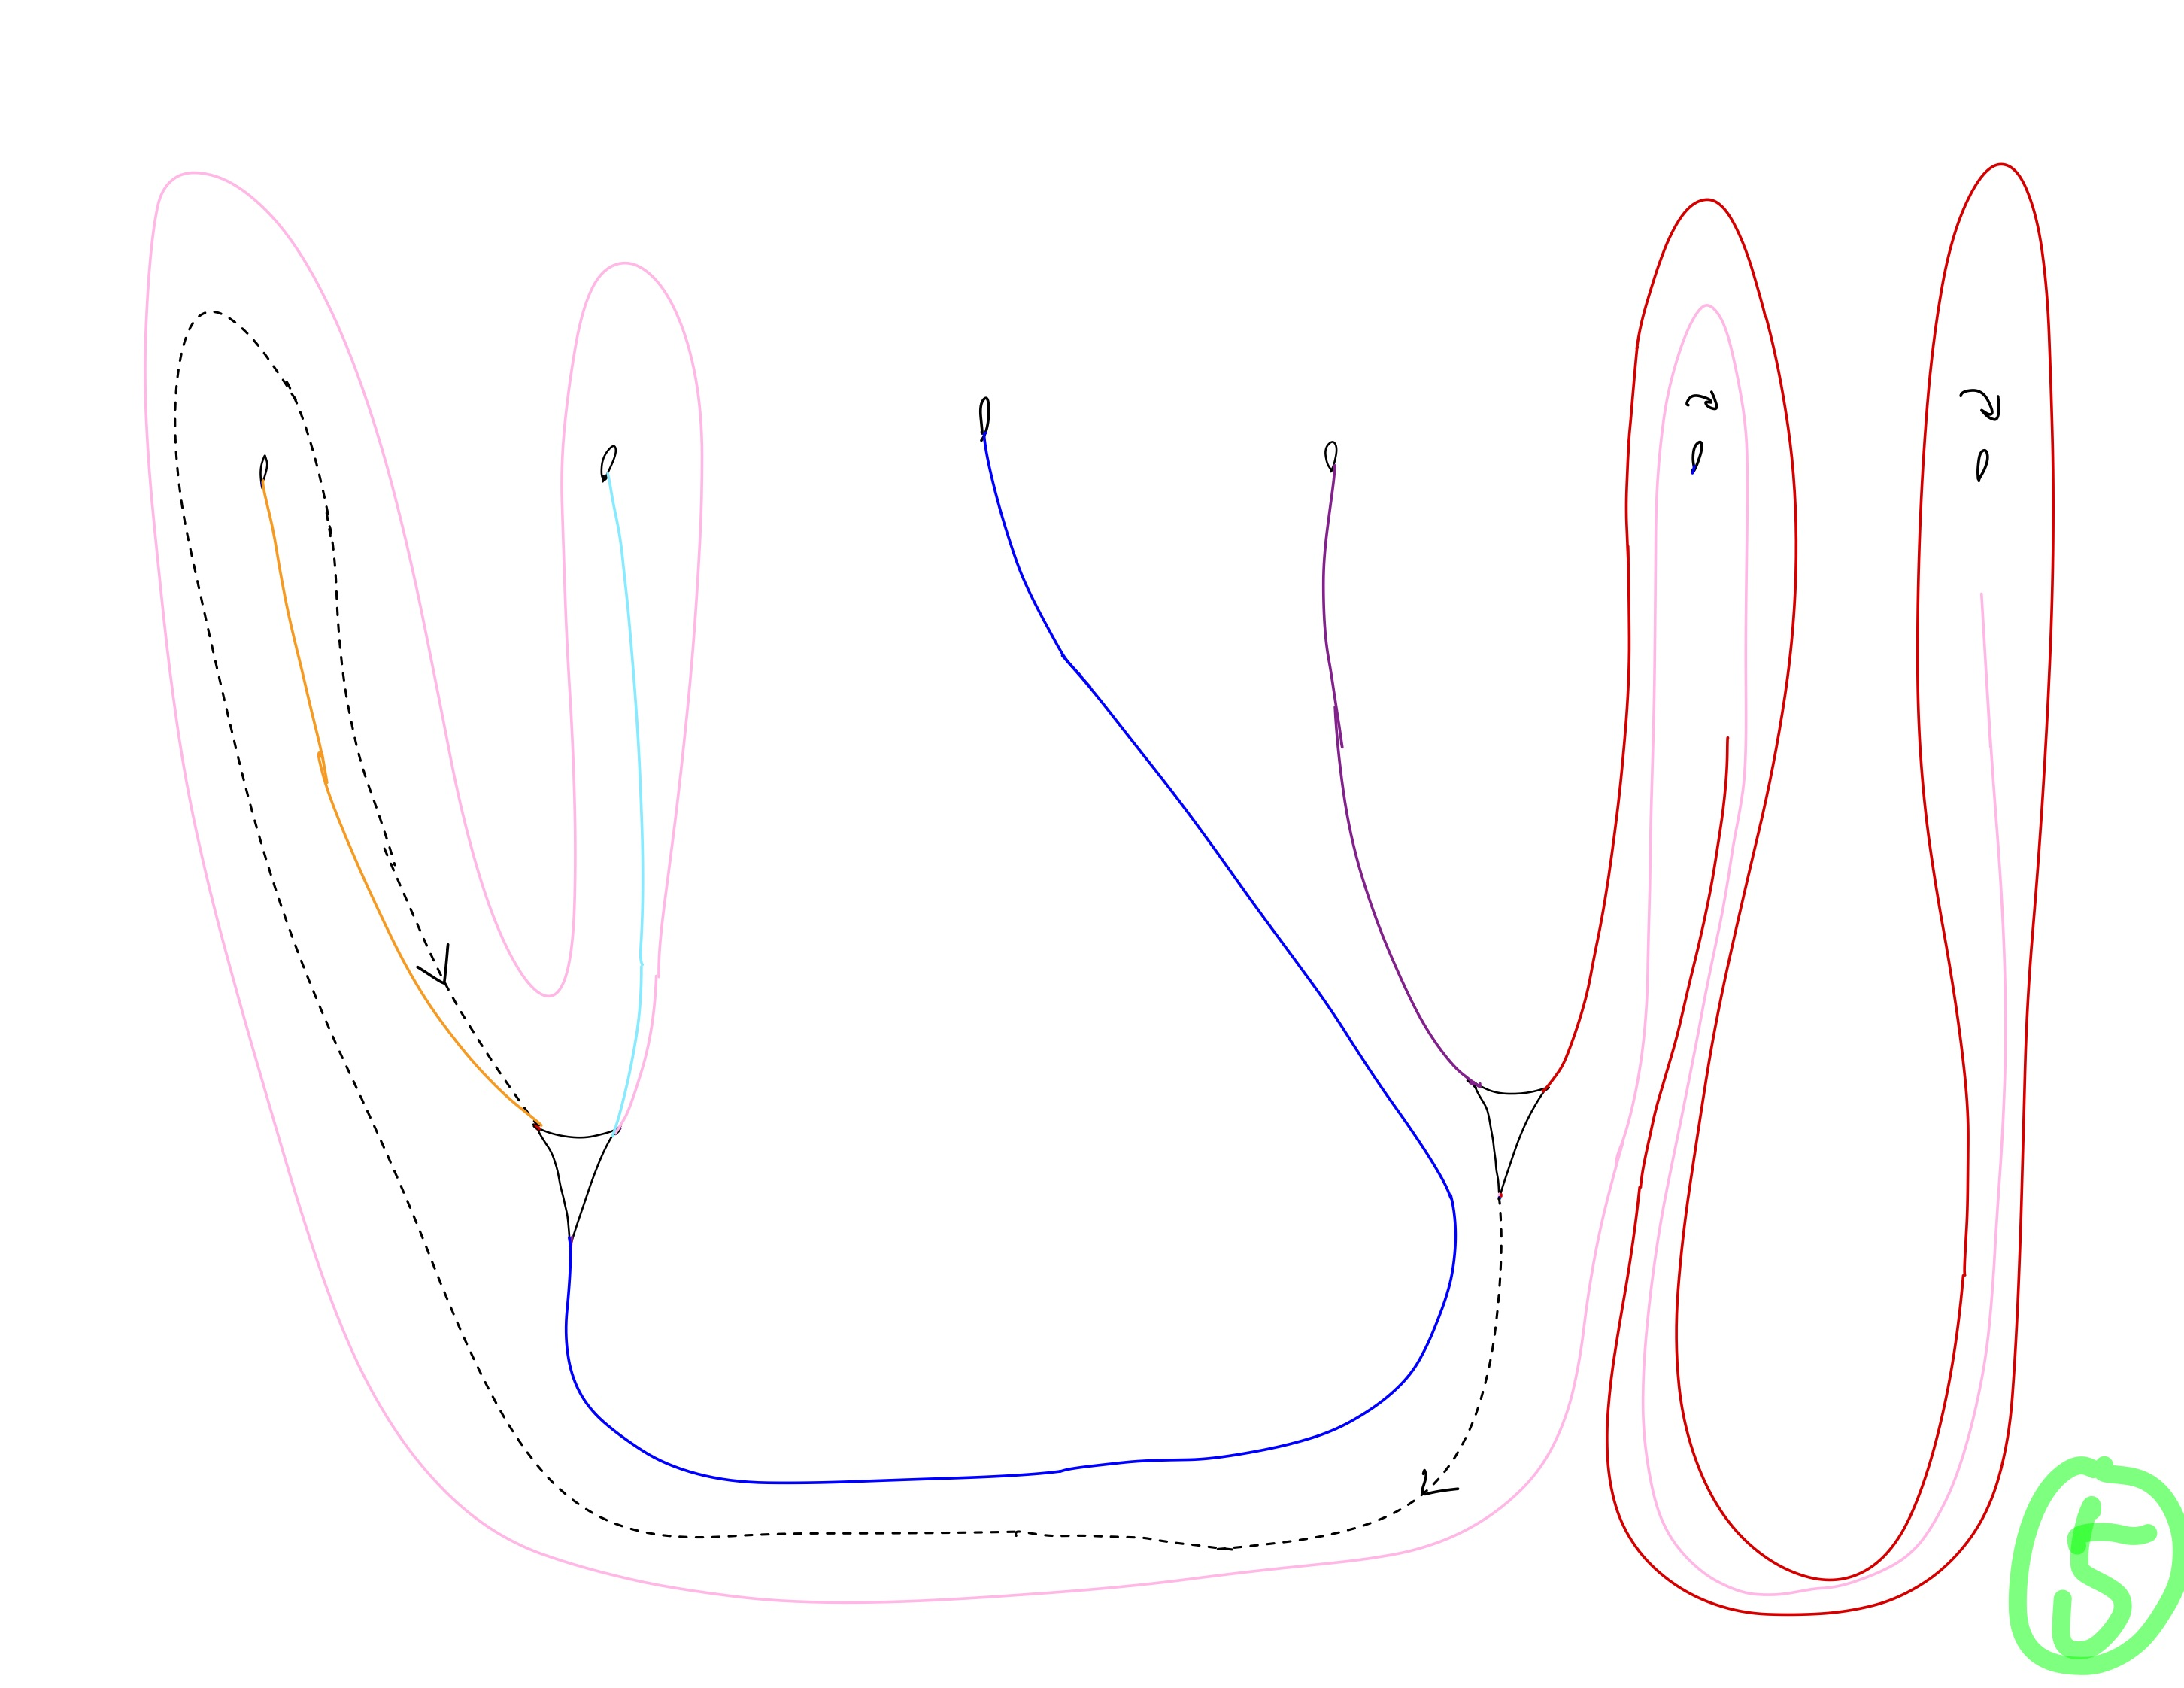
\includegraphics[width=\linewidth, height=0.45\textheight, keepaspectratio]{figures_braid/figures_track_17/Track 17 Braid 5 Boke-1.jpg}
    \caption{Train Track Map Candidate Family 5 (Boke) of Track 17.}
    \label{fig:track17_braid_b17_5_map}
\end{figure*}

The inverse of the following braid carries this family of train track maps:
\[
b_5^{17} = \sigma_{5}^{k} \sigma_{1} \sigma_{2} \sigma_{5}^{-1} \sigma_{4}^{-1} \sigma_{3}^{-1} \sigma_{2}^{-1} \sigma_{1}^{-1} \sigma_{1}^{-1} \circ P \circ \Lambda_6
\]

This is shown in Figure \ref{fig:track17_braid_b17_5}.

\begin{figure*}[p]
    \centering
    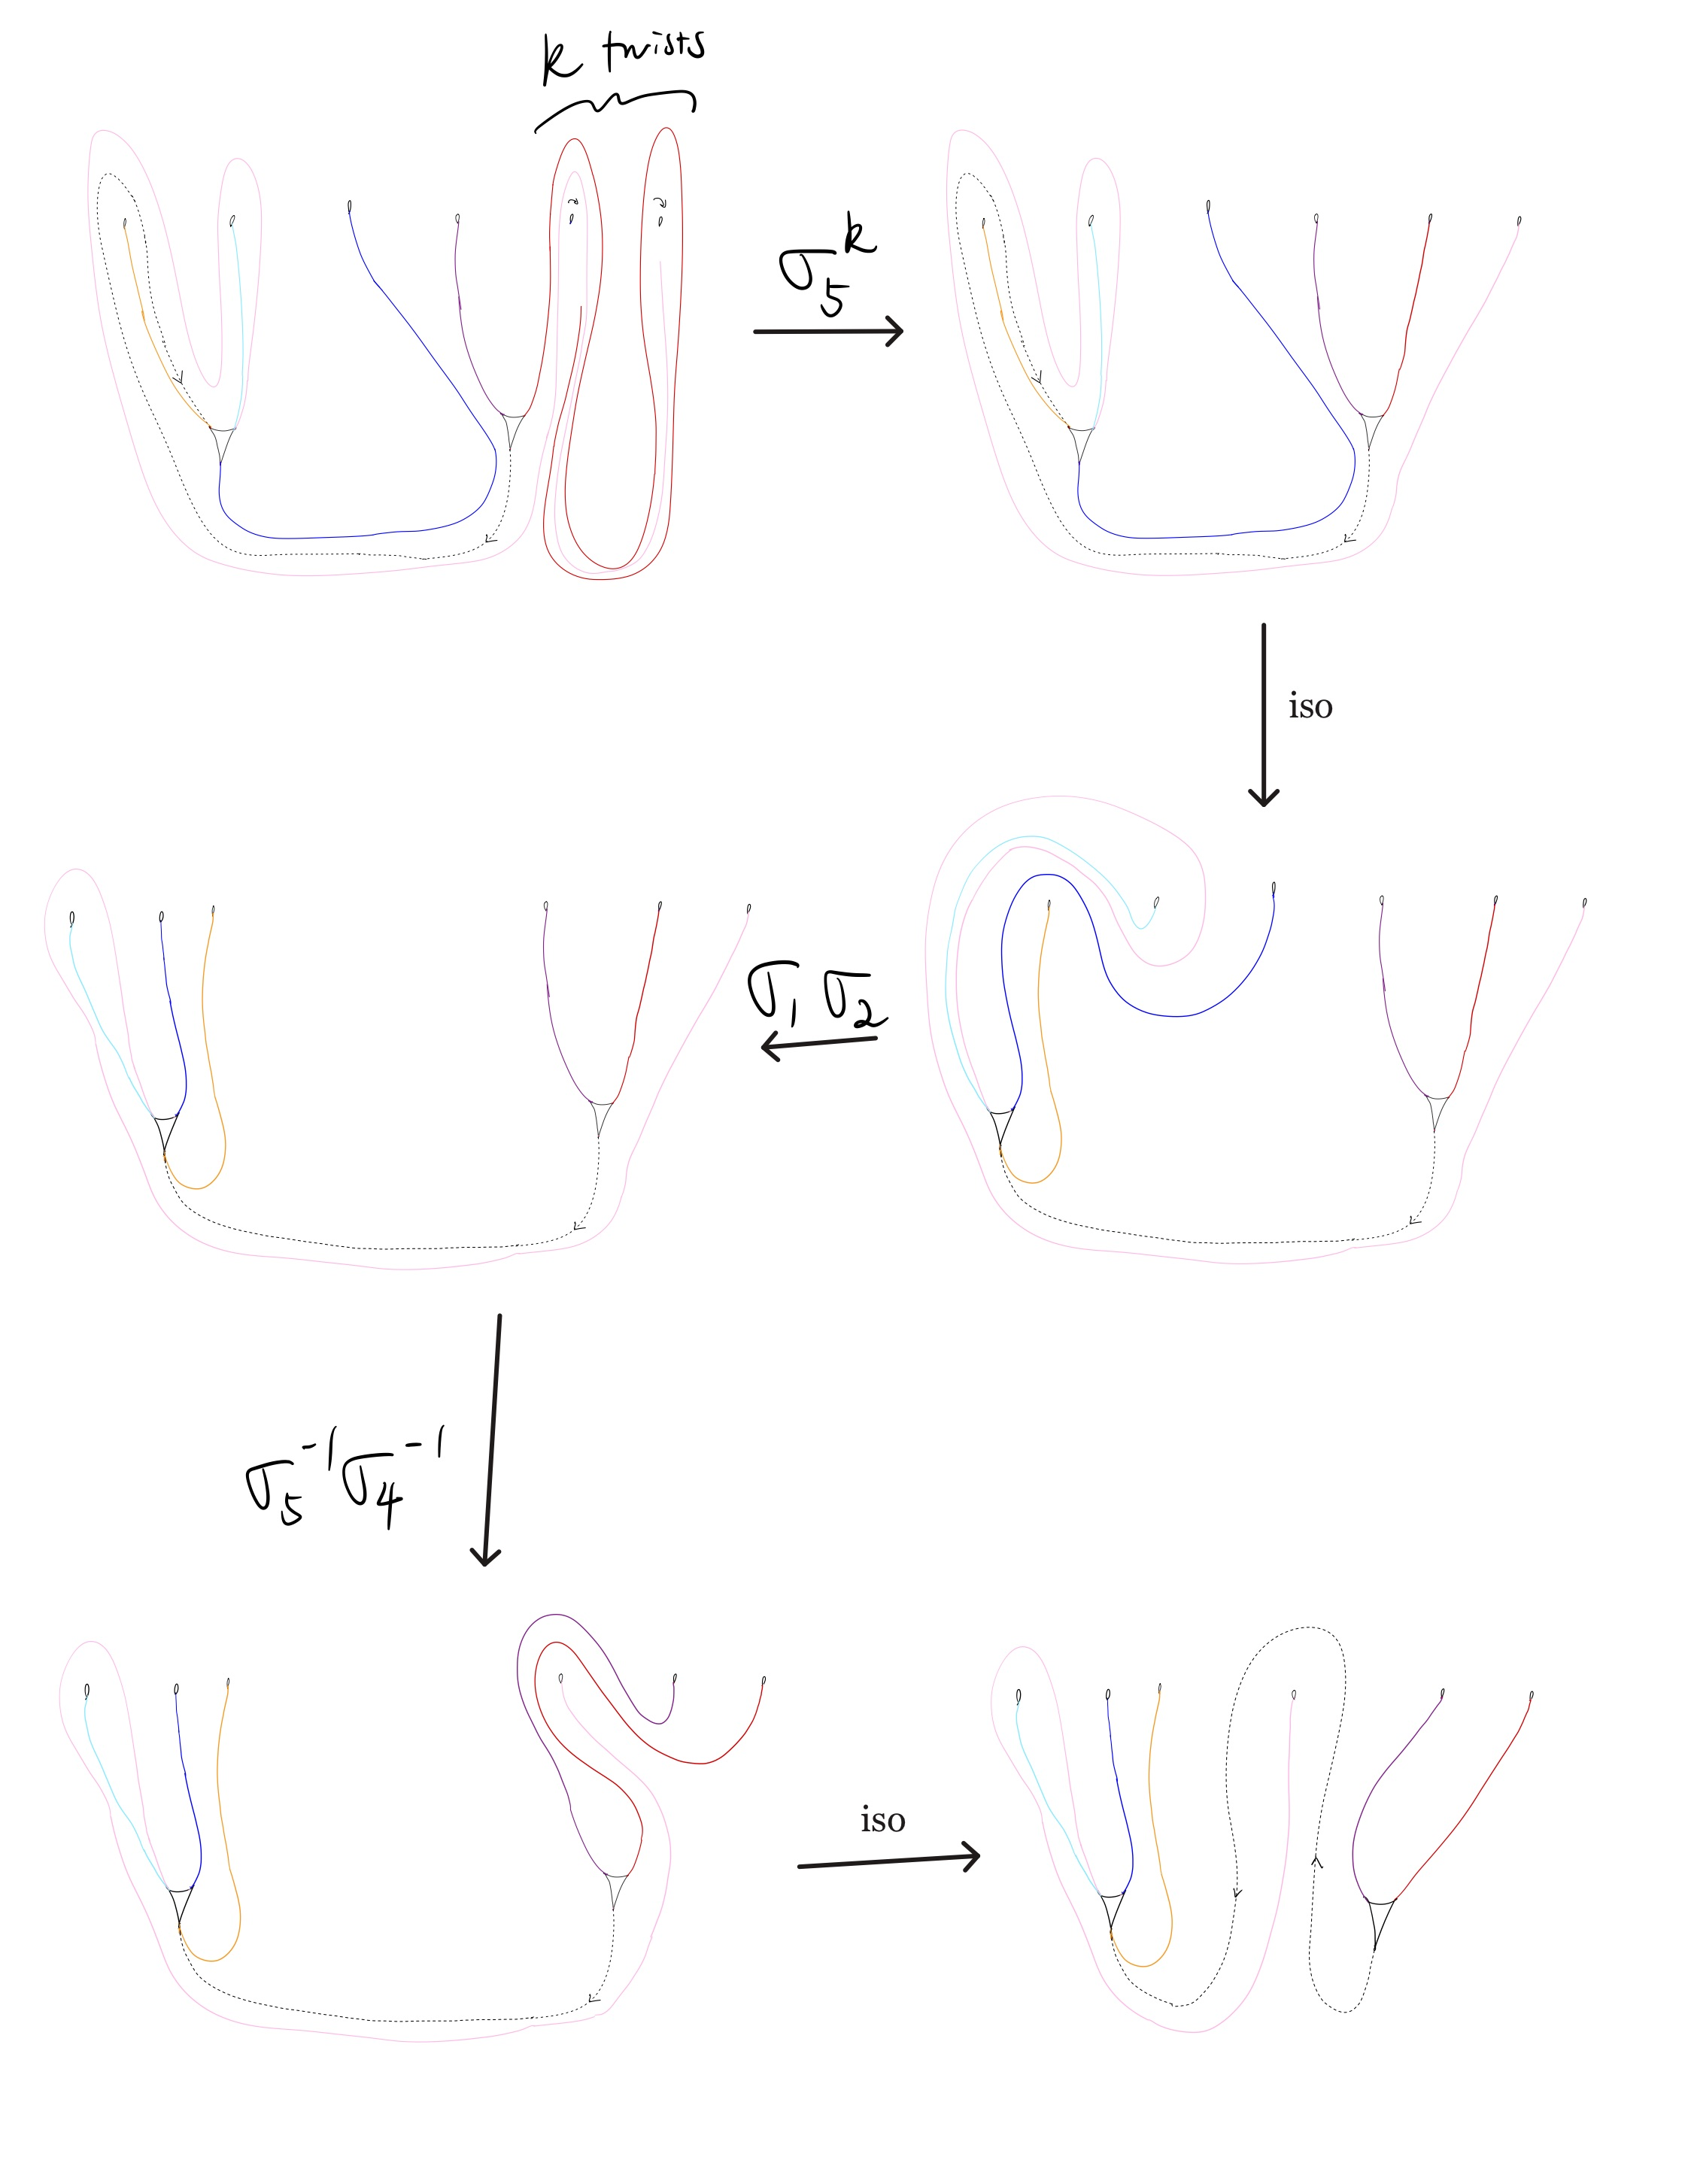
\includegraphics[width=\linewidth, height=0.45\textheight, keepaspectratio]{figures_braid/figures_track_17/Track 17 Braid 5 Boke-2.jpg}\\
    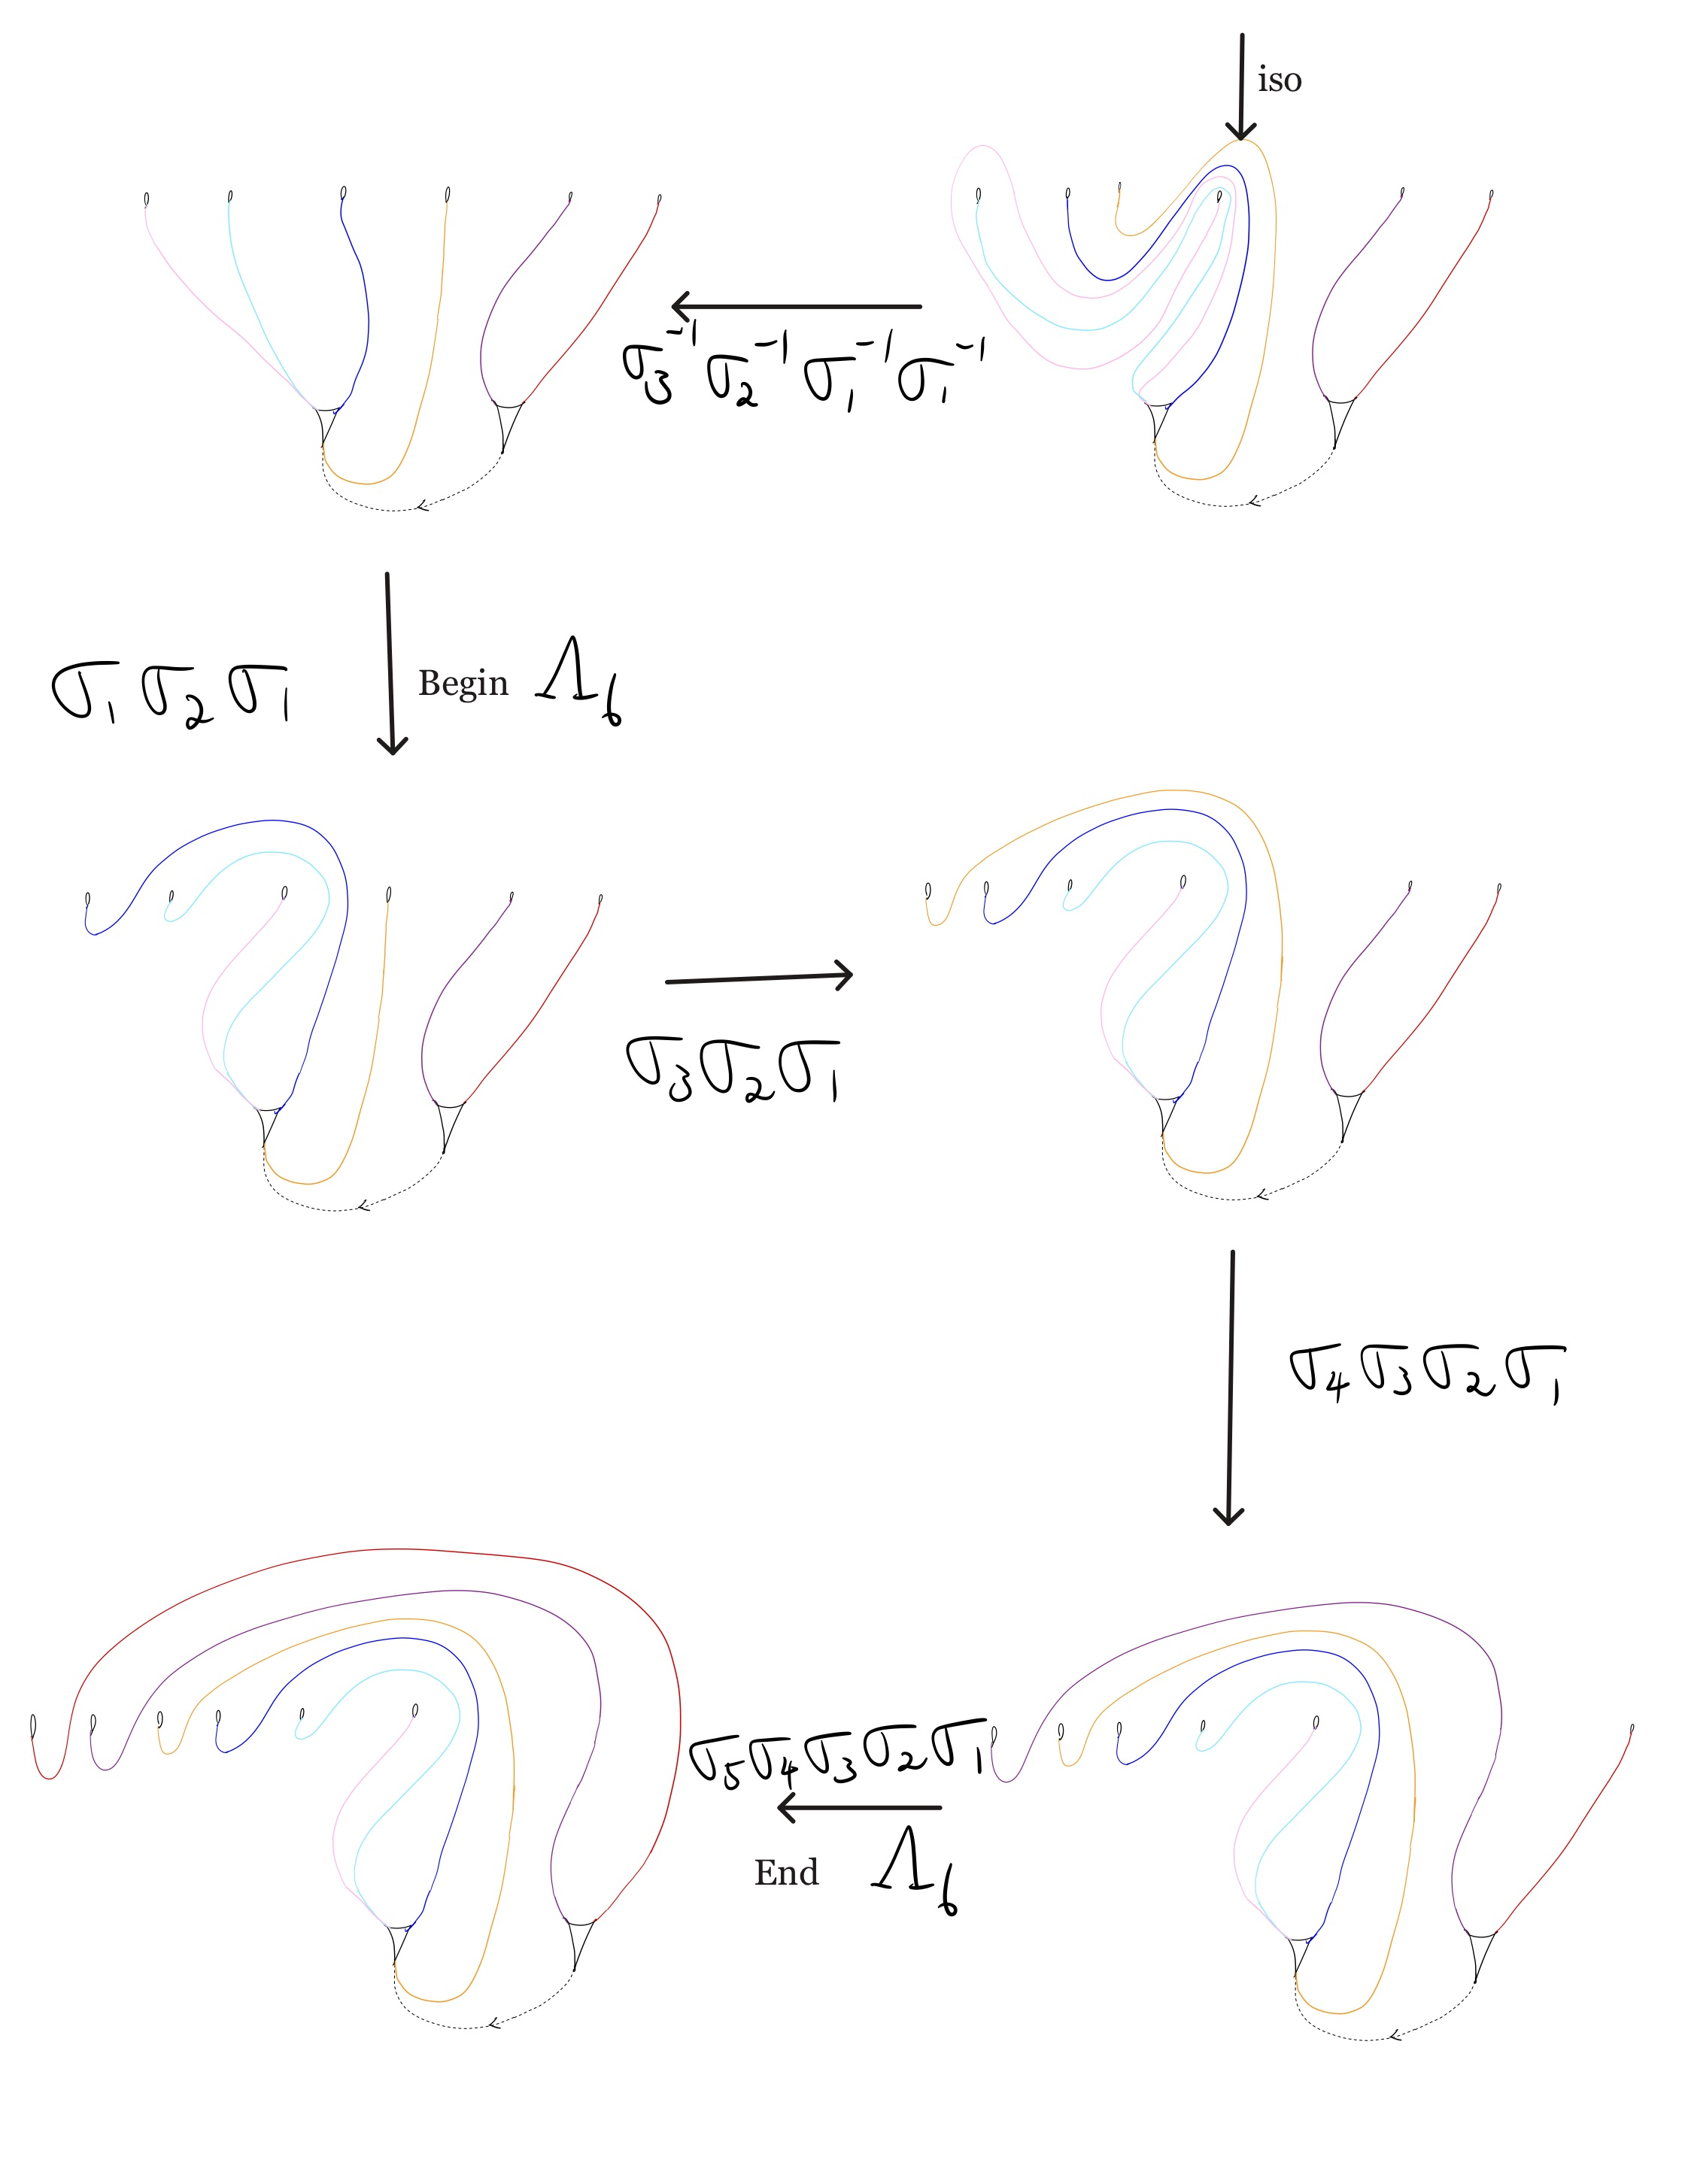
\includegraphics[width=\linewidth, height=0.45\textheight, keepaspectratio]{figures_braid/figures_track_17/Track 17 Braid 5 Boke-3.jpg}
    \caption{This sequence shows the inverse of the braid $b_5^{17}$ carries Train Track Candidate Family 5 (first half).}
    \label{fig:track17_braid_b17_5}
\end{figure*}

\begin{figure*}[p]
    \centering
    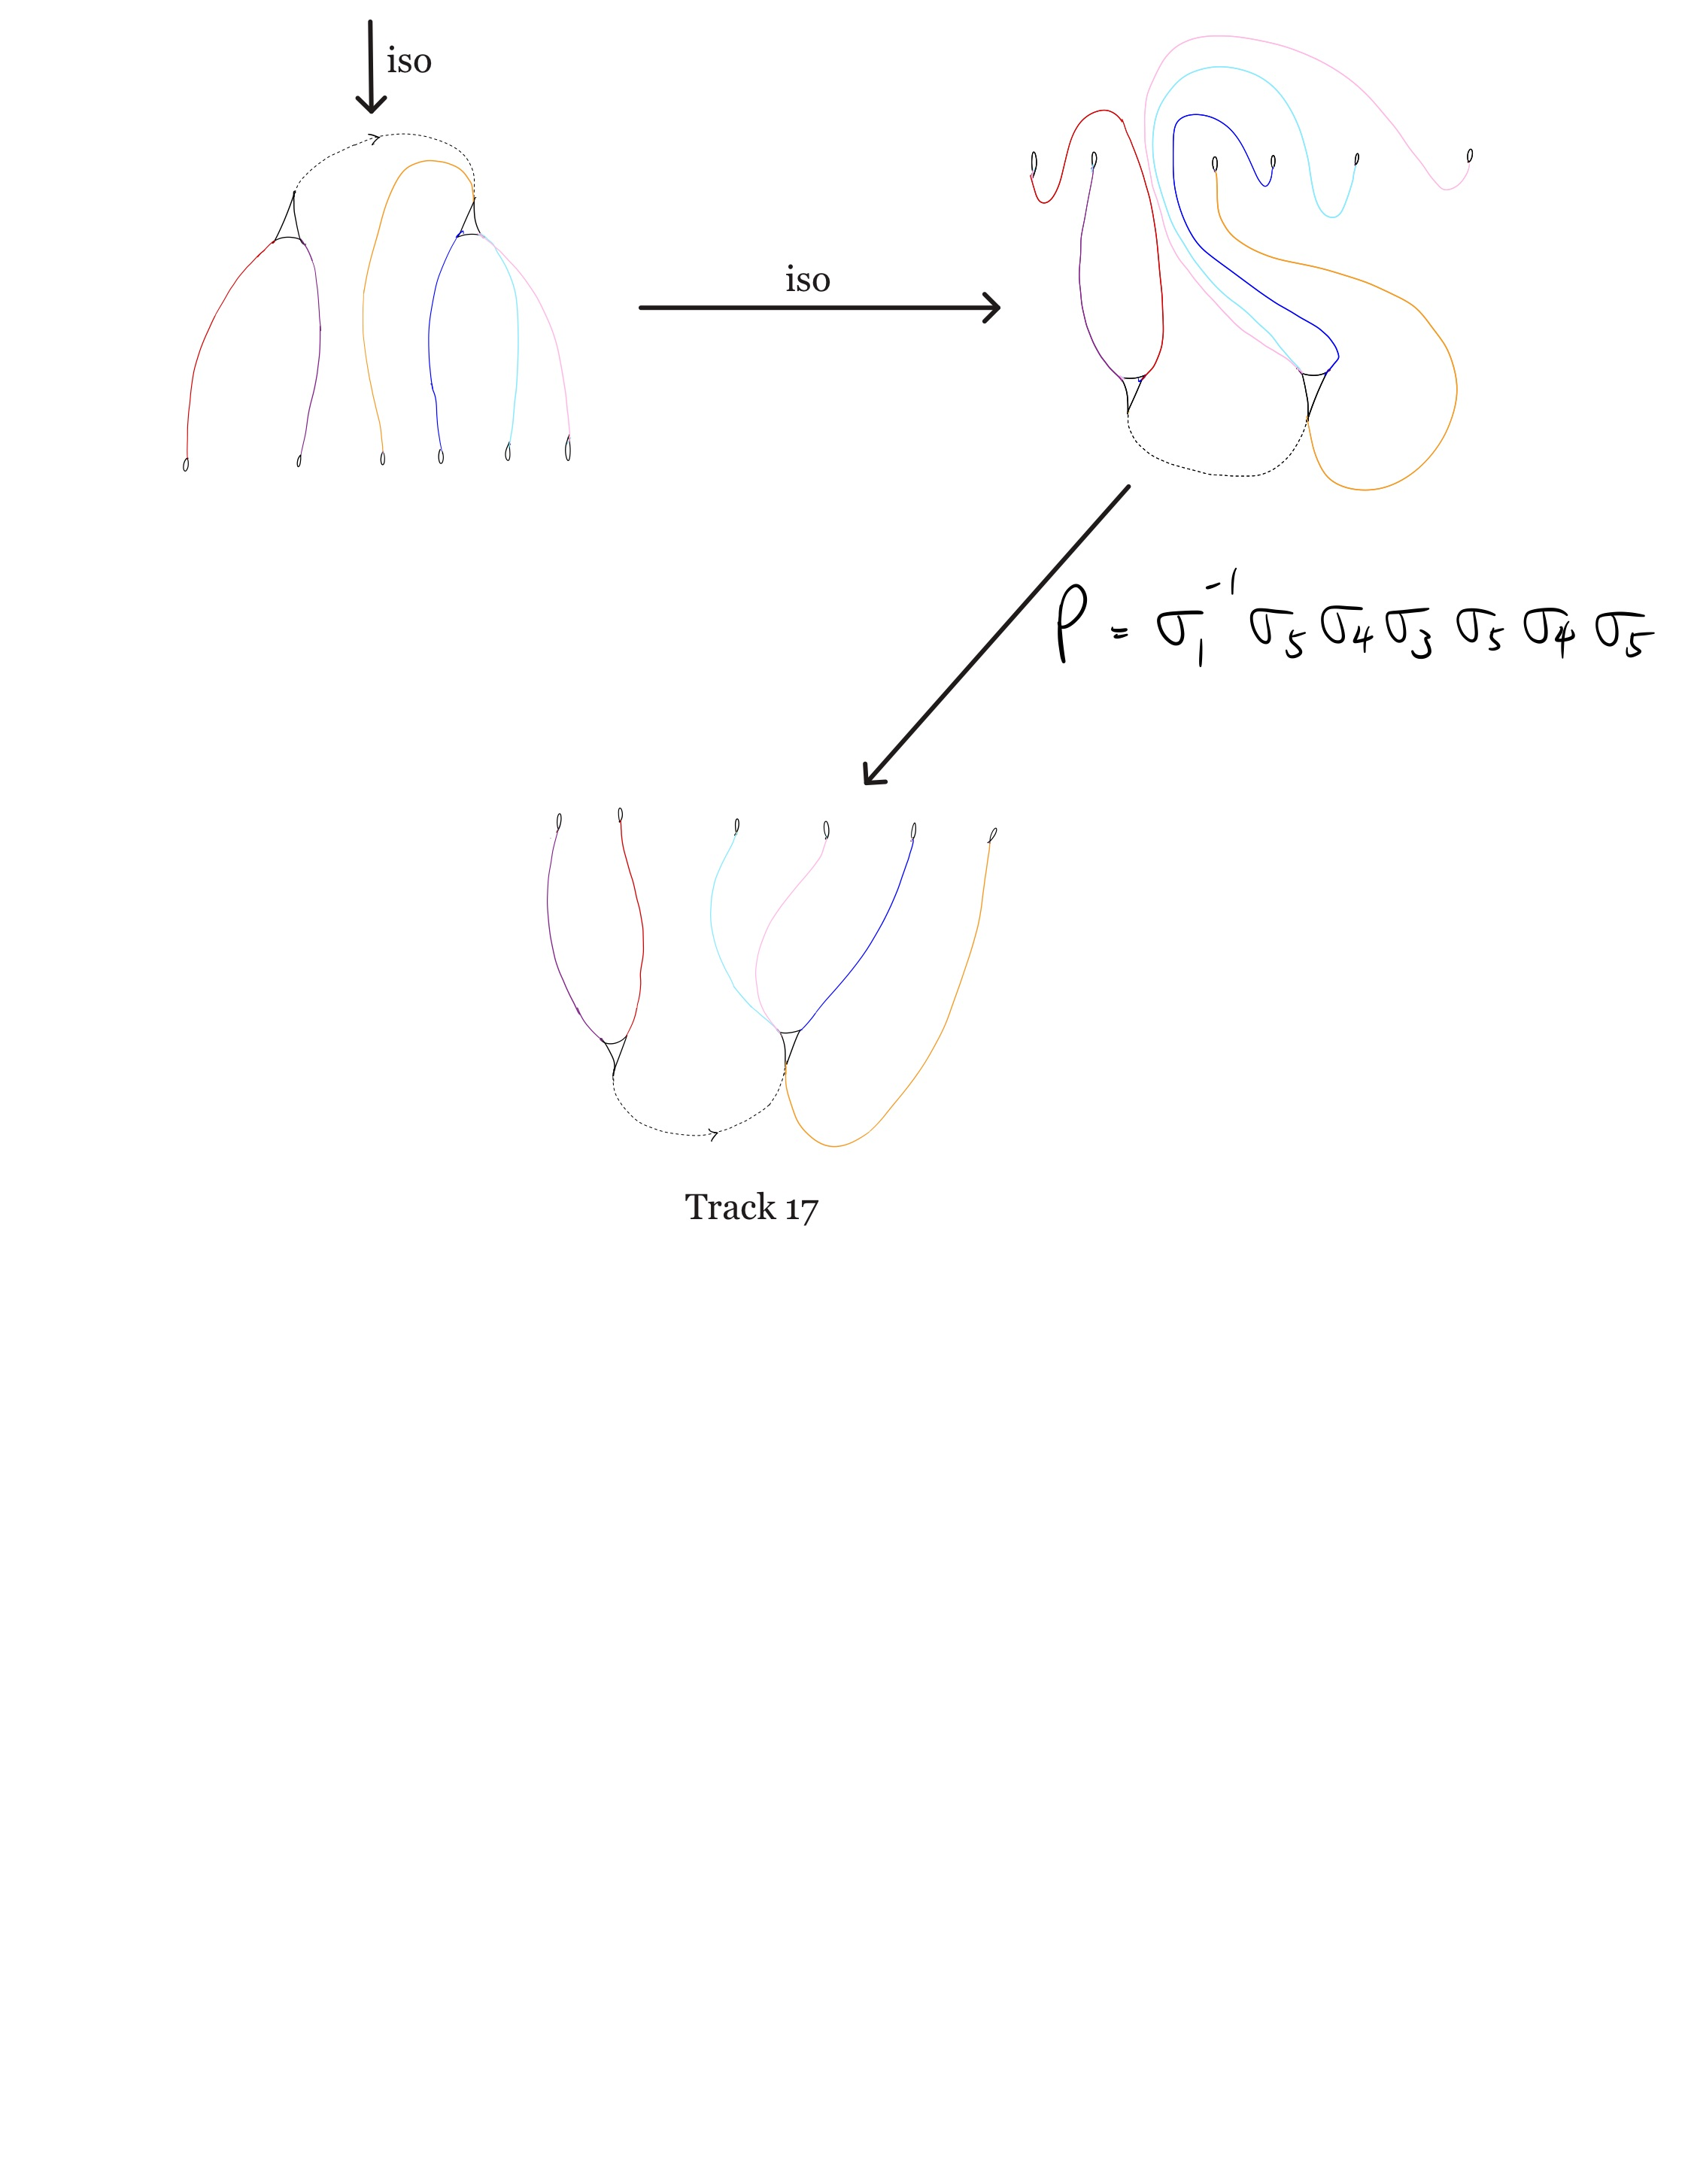
\includegraphics[width=\linewidth, height=0.45\textheight, keepaspectratio]{figures_braid/figures_track_17/Track 17 Braid 5 Boke-4.jpg}
    \caption{Continuation of Figure \ref{fig:track17_braid_b17_5}: the inverse of $b_5^{17}$ carries Train Track Candidate Family 5 (second half).}
    \label{fig:track17_braid_b17_5_cont}
\end{figure*}

\clearpage

\section{Candidate Family 6 (Boke)}\label{sec:track17_boke_6}
Train Track Map Candidate Family 6 of Track 17 is shown in Figure \ref{fig:track17_braid_b17_6_map}. See Section \ref{Boke} for details. This is a parametric family indexed by an integer twist parameter $k \in \mathbb{Z}_{\geq 0}$.

\begin{figure*}[ht]
    \centering
    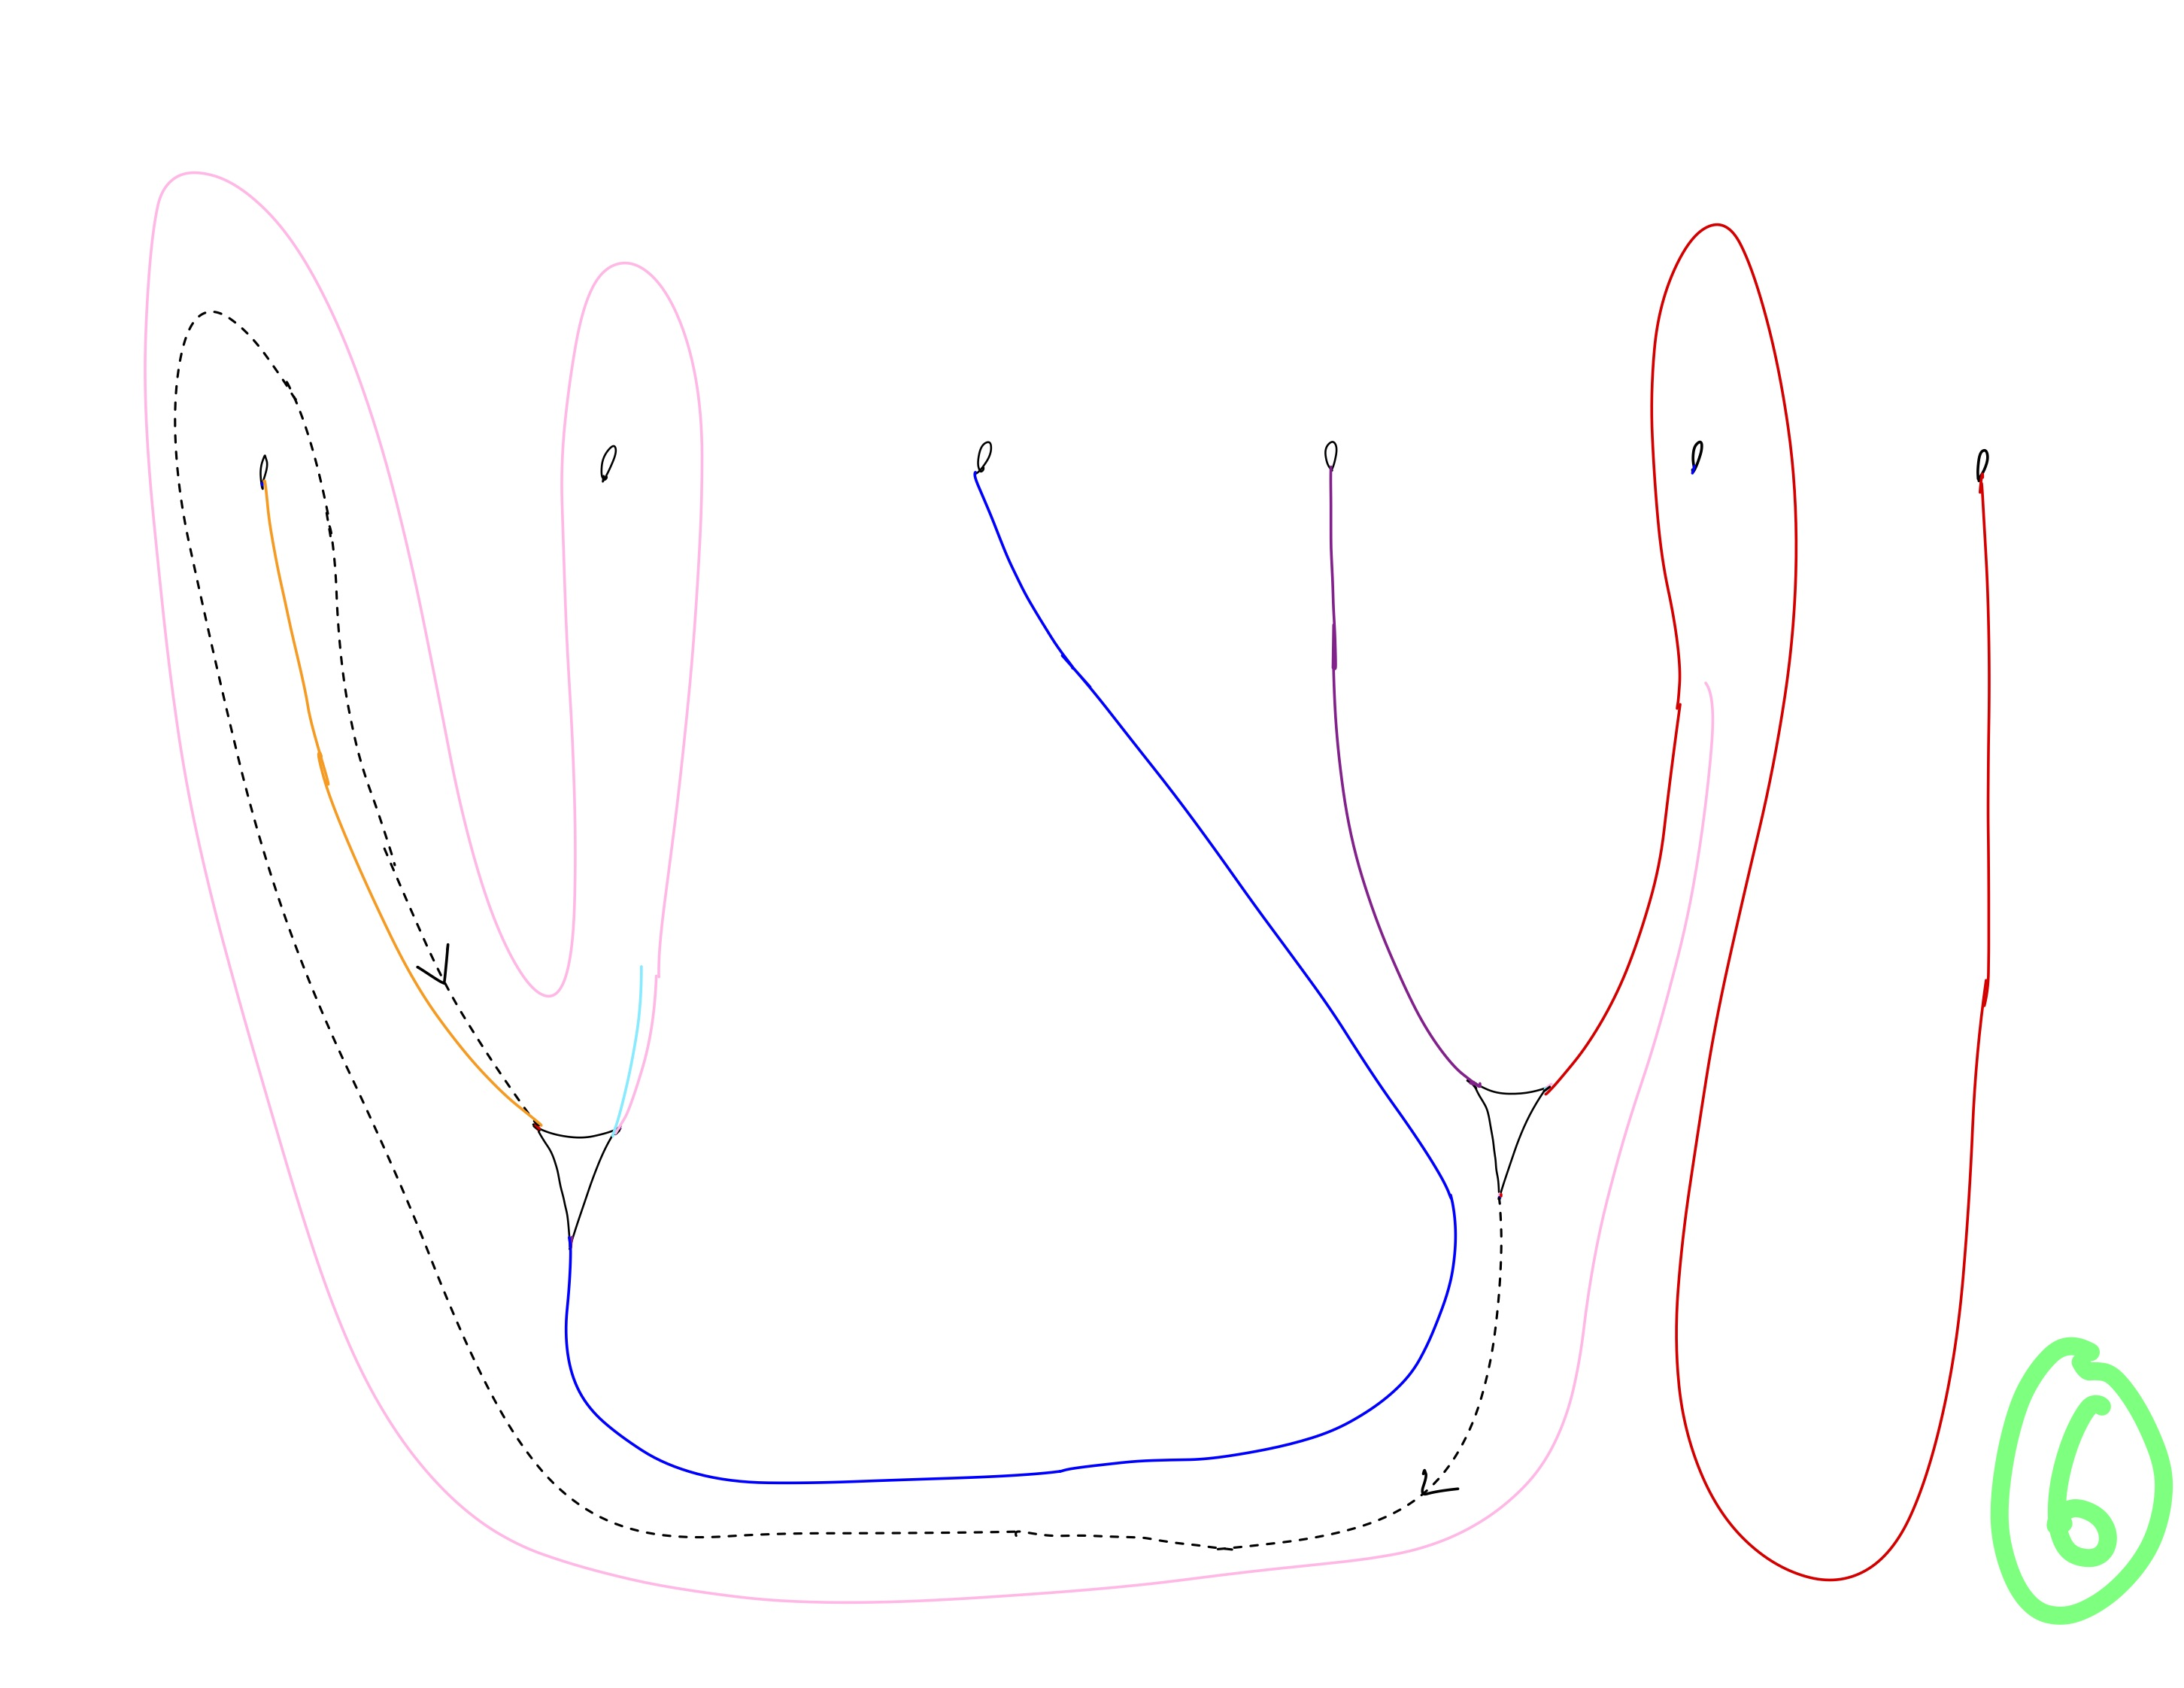
\includegraphics[width=\linewidth, height=0.45\textheight, keepaspectratio]{figures_braid/figures_track_17/Track 17 Braid 6 Boke-1.jpg}
    \caption{Train Track Map Candidate Family 6 (Boke) of Track 17.}
    \label{fig:track17_braid_b17_6_map}
\end{figure*}

The inverse of the following braid carries this family of train track maps:
\[
b_6^{17} = \sigma_{1} \sigma_{2} \sigma_{4}^{-1} \sigma_{1} \sigma_{2} \sigma_{3}^{-k} \sigma_{2} \sigma_{3} \sigma_{1} \sigma_{2} \sigma_{1} \sigma_{1} \circ P \circ \Lambda_6
\]

This is shown in Figure \ref{fig:track17_braid_b17_6}.

\begin{figure*}[p]
    \centering
    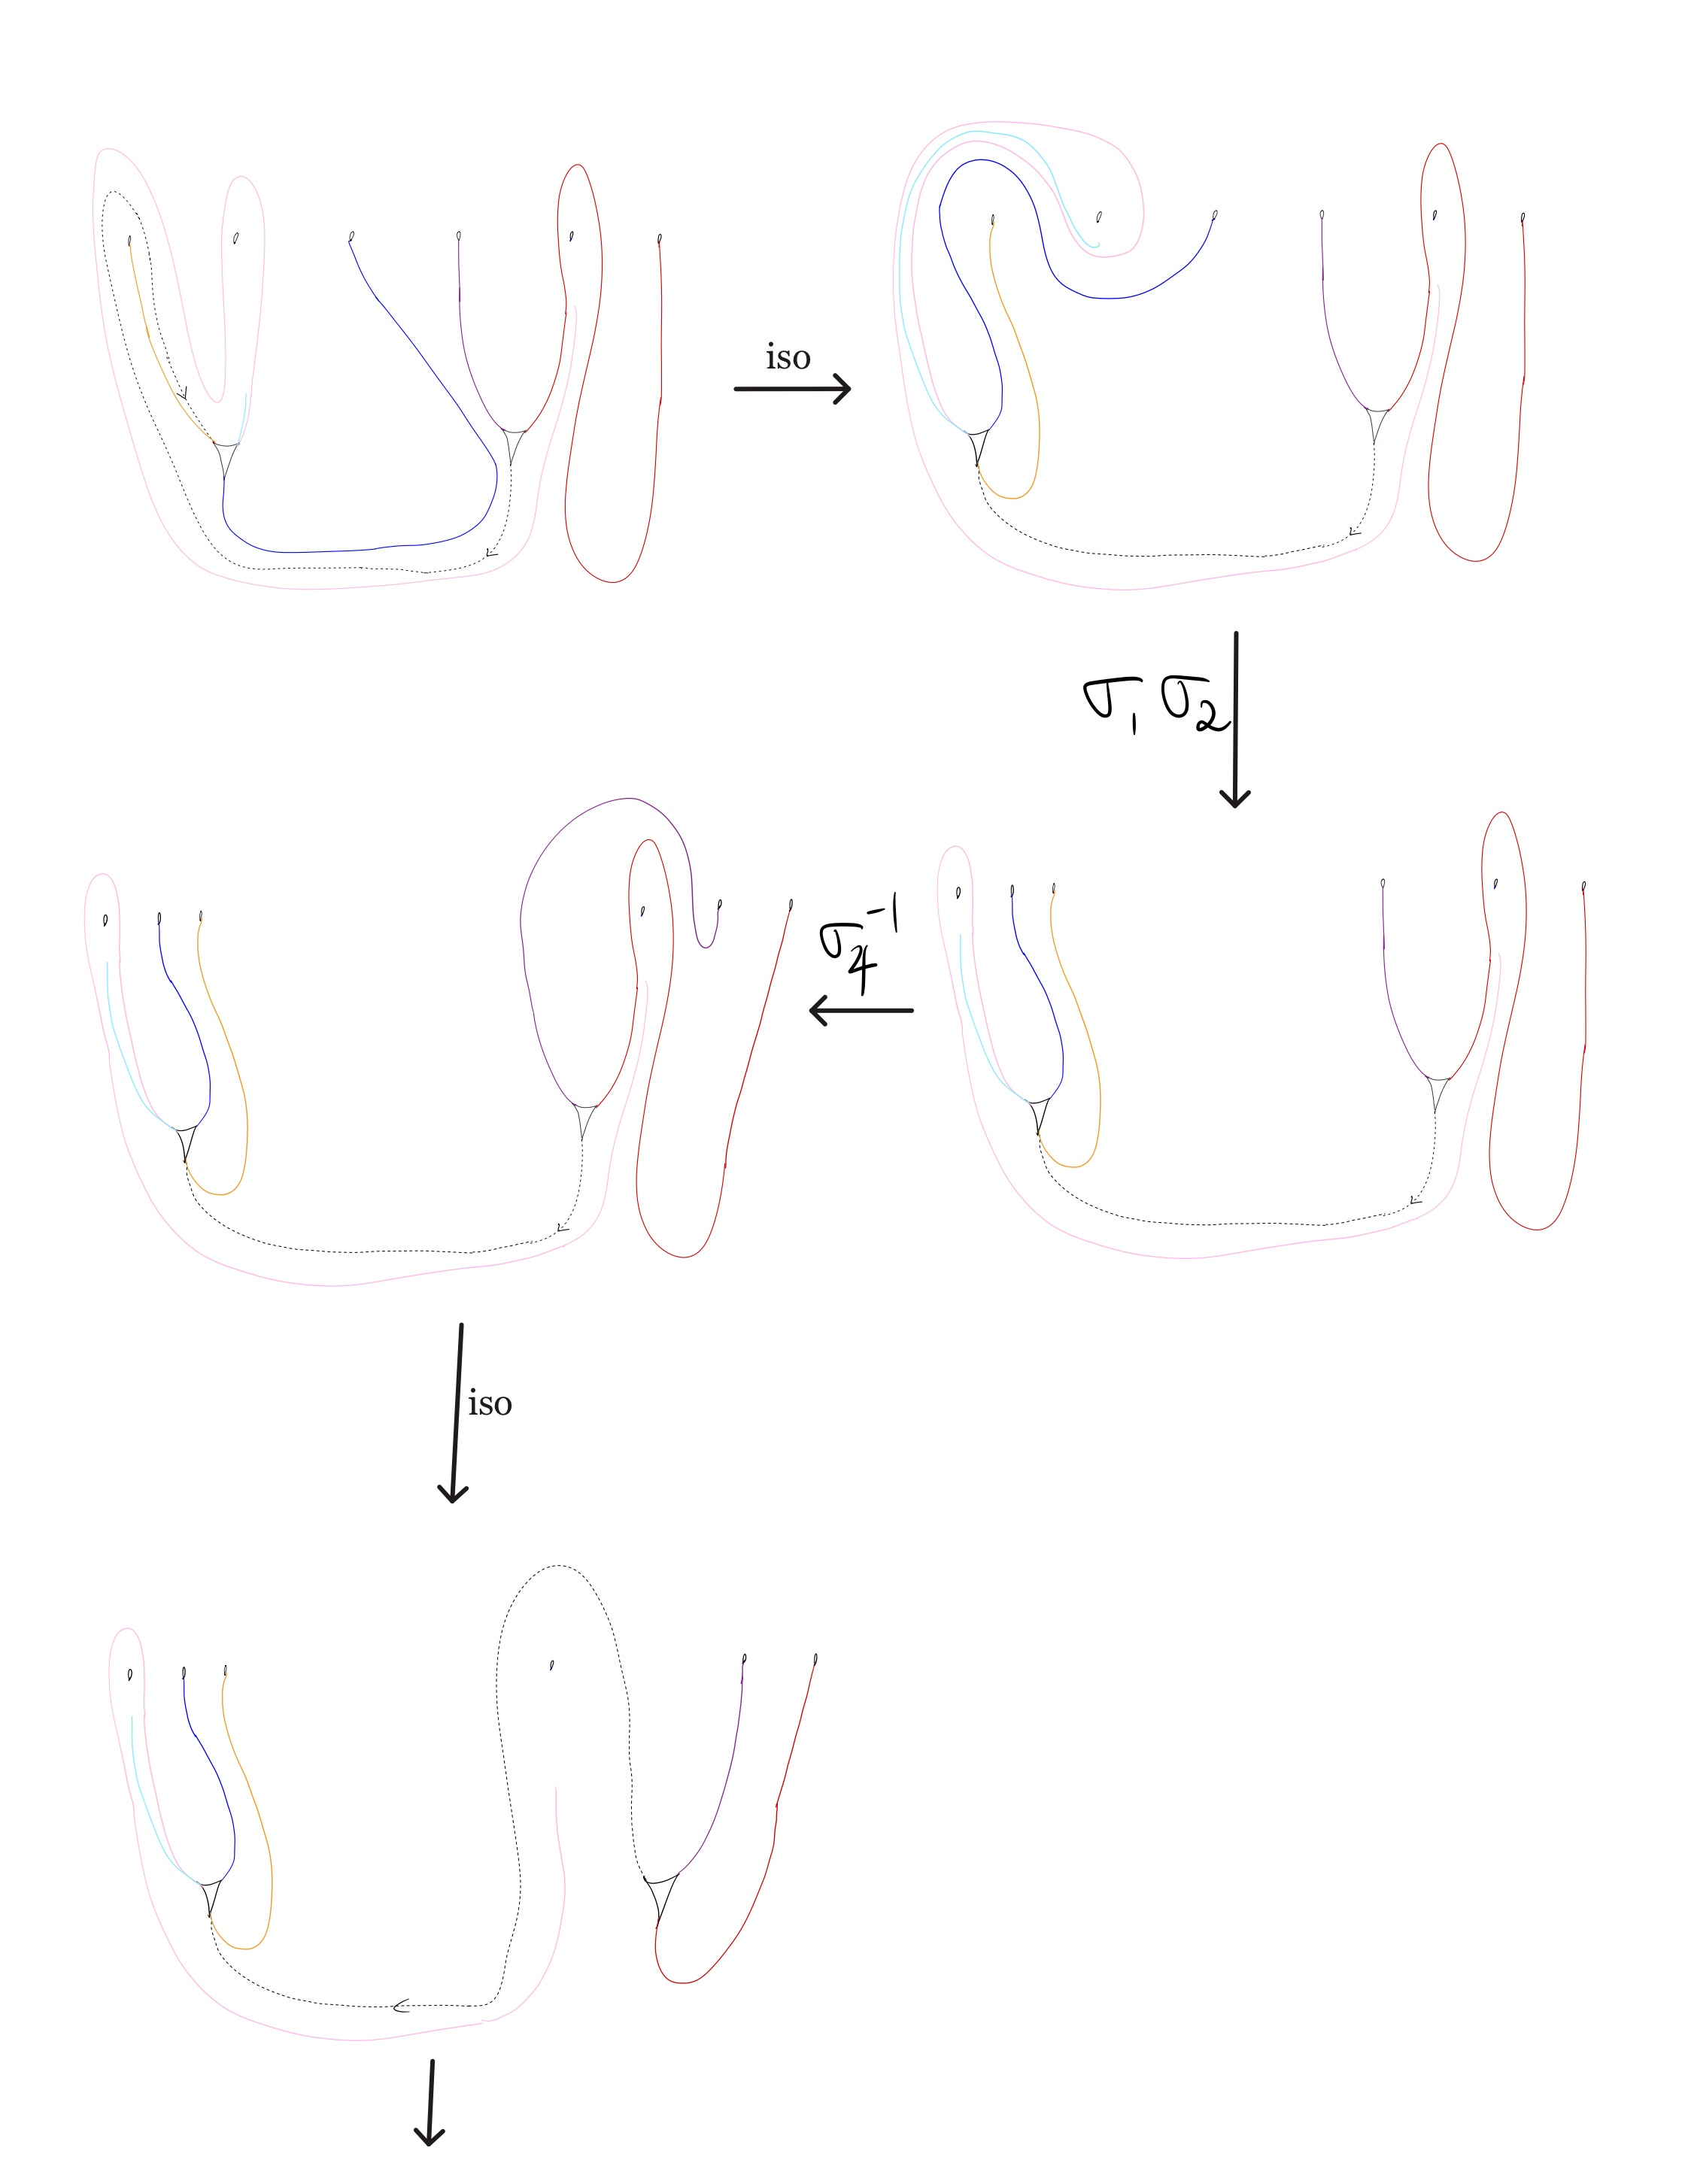
\includegraphics[width=\linewidth, height=0.45\textheight, keepaspectratio]{figures_braid/figures_track_17/Track 17 Braid 6 Boke-2.jpg}\\
    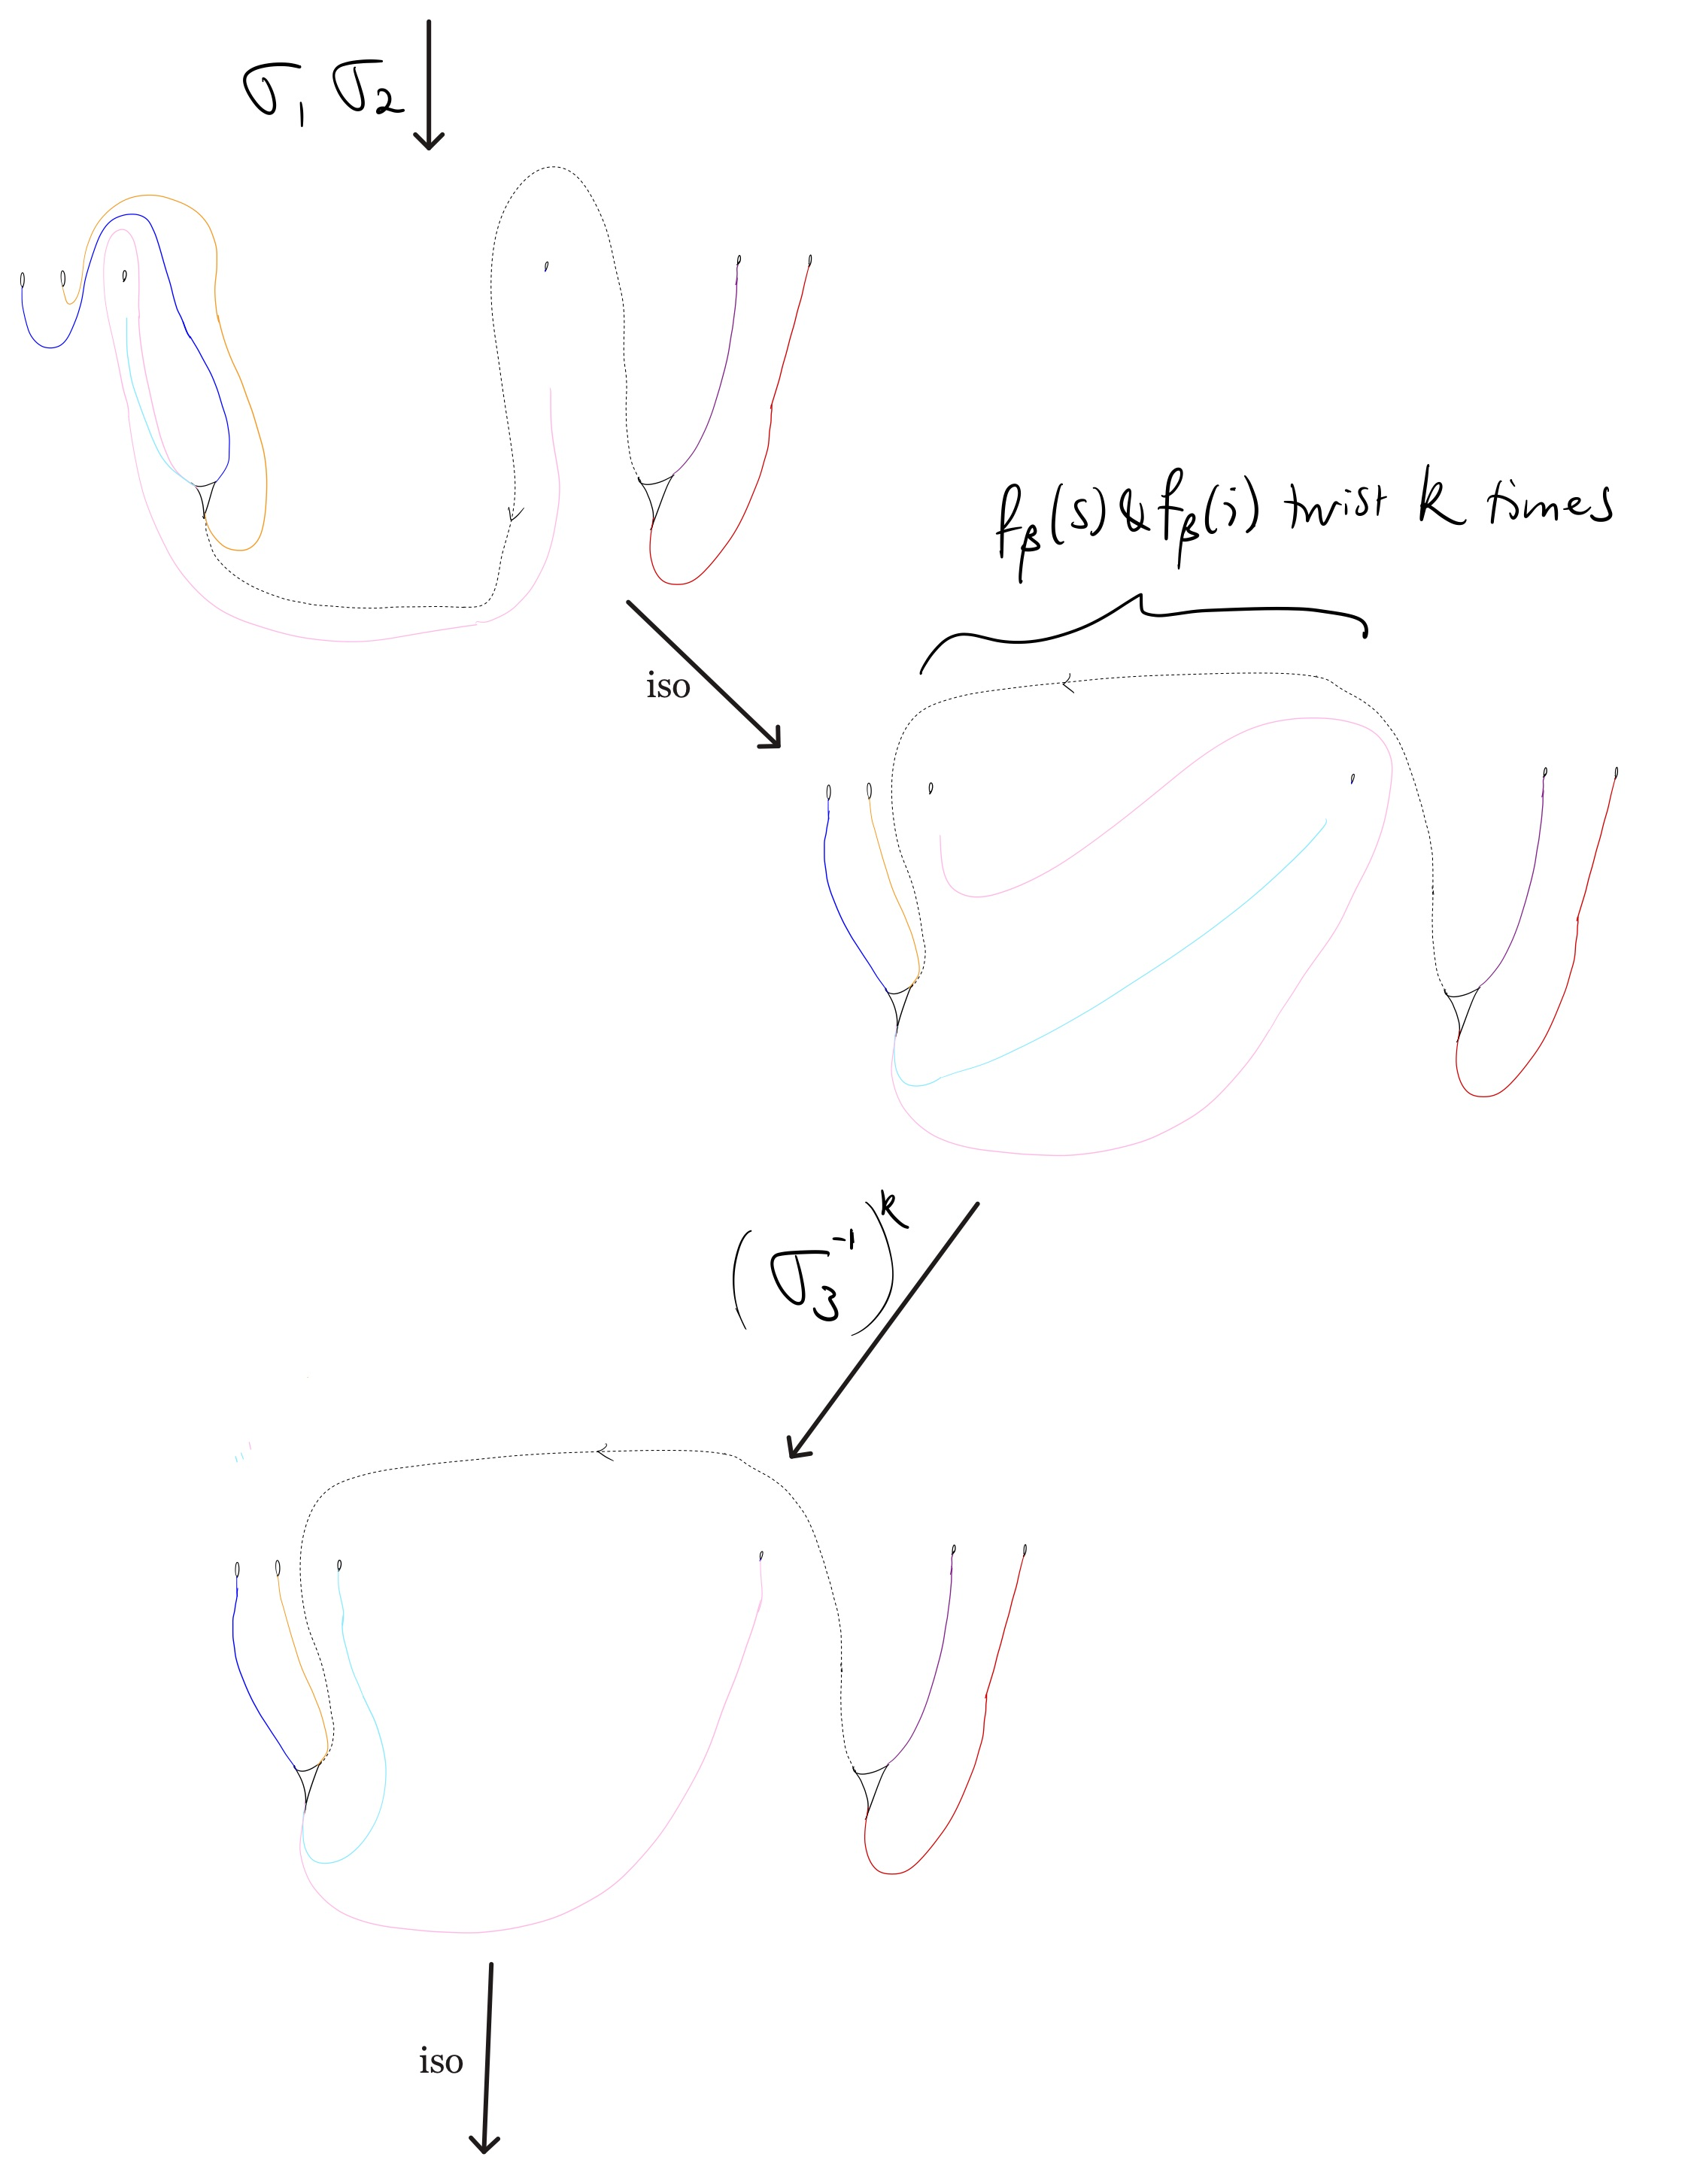
\includegraphics[width=\linewidth, height=0.45\textheight, keepaspectratio]{figures_braid/figures_track_17/Track 17 Braid 6 Boke-3.jpg}
    \caption{This sequence shows the inverse of the braid $b_6^{17}$ carries Train Track Candidate Family 6 (first half).}
    \label{fig:track17_braid_b17_6}
\end{figure*}

\begin{figure*}[p]
    \centering
    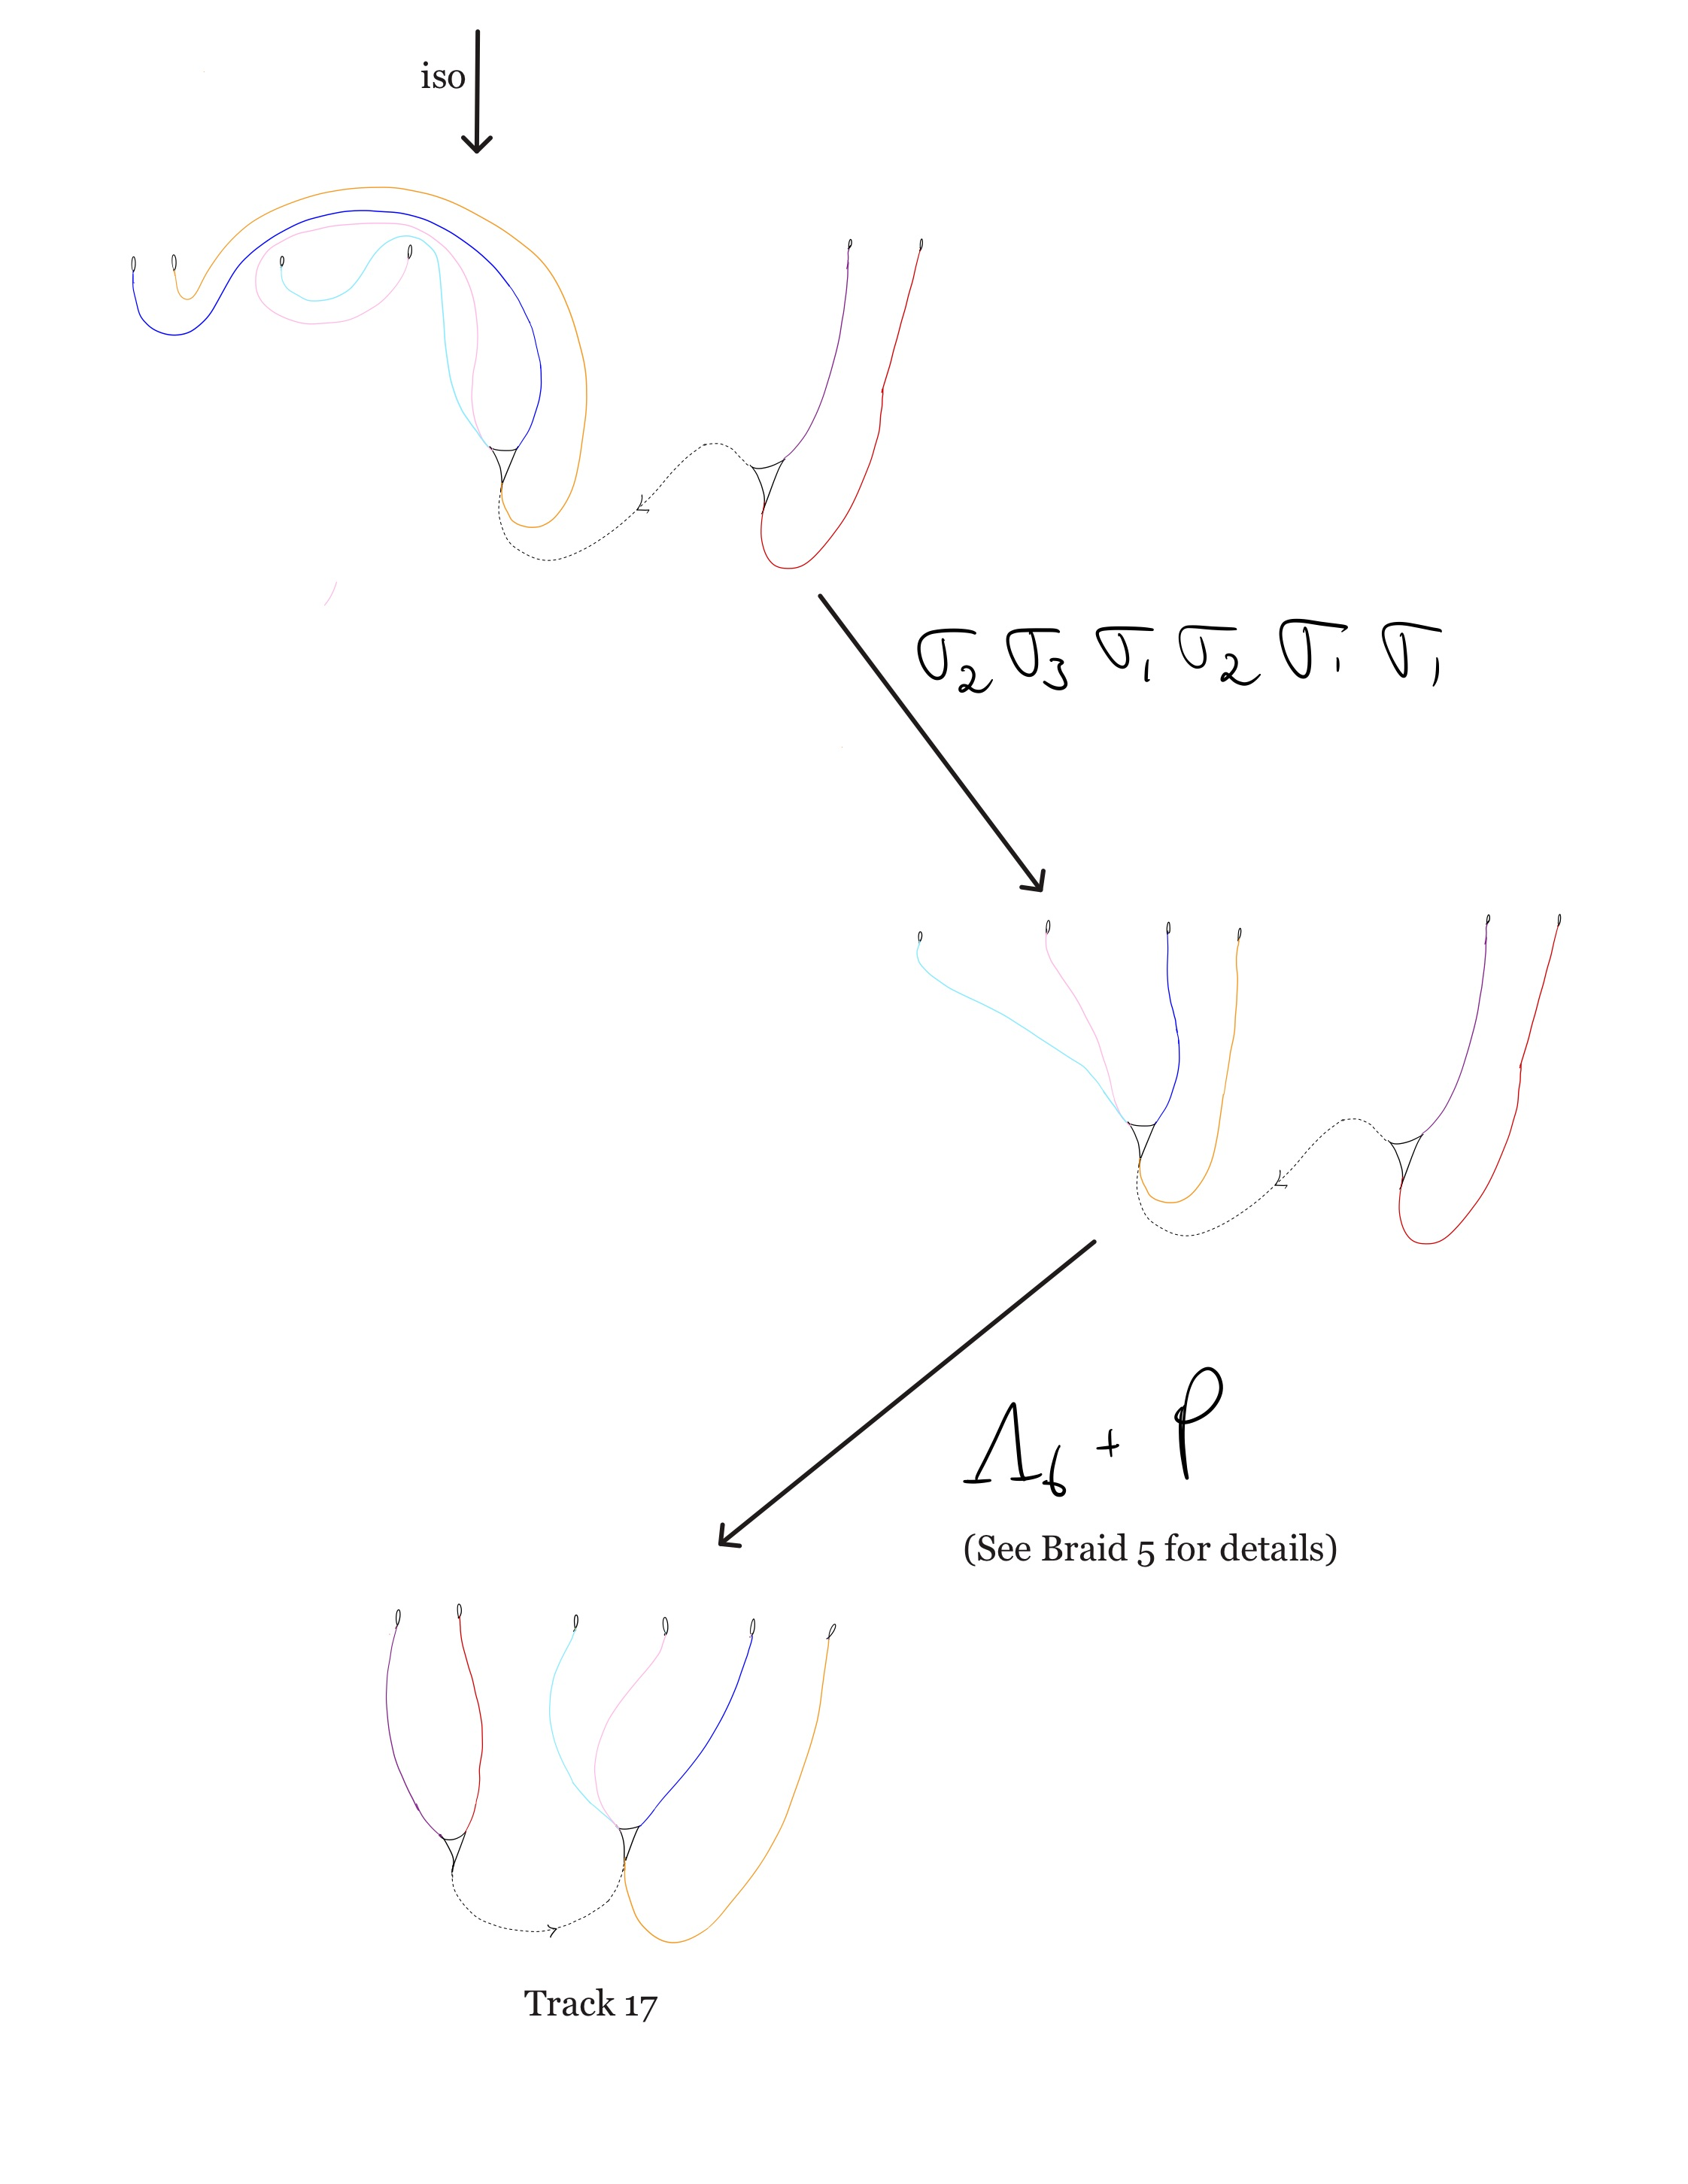
\includegraphics[width=\linewidth, height=0.45\textheight, keepaspectratio]{figures_braid/figures_track_17/Track 17 Braid 6 Boke-4.jpg}
    \caption{Continuation of Figure \ref{fig:track17_braid_b17_6}: the inverse of $b_6^{17}$ carries Train Track Candidate Family 6 (second half).}
    \label{fig:track17_braid_b17_6_cont}
\end{figure*}

\clearpage